%% LyX 2.1.4 created this file.  For more info, see http://www.lyx.org/.
%% Do not edit unless you really know what you are doing.
\documentclass{UNCC-thesis}
\usepackage[T1]{fontenc}
\usepackage[latin9]{inputenc}
\setcounter{secnumdepth}{3}
\usepackage{array}
\usepackage{algorithmic}
\usepackage[ruled,vlined]{algorithm2e}
\usepackage{float}
\usepackage{subfigure}
\usepackage{graphicx}
\usepackage{nomencl}
\usepackage{amsmath}
\newtheorem{definition}{Definition}

% the following is useful when we have the old nomencl.sty package
\providecommand{\printnomenclature}{\printglossary}
\providecommand{\makenomenclature}{\makeglossary}
\makenomenclature

\makeatletter

%%%%%%%%%%%%%%%%%%%%%%%%%%%%%% LyX specific LaTeX commands.
%% Because html converters don't know tabularnewline
\providecommand{\tabularnewline}{\\}

%%%%%%%%%%%%%%%%%%%%%%%%%%%%%% User specified LaTeX commands.
% If you are using MikTeX on Windows and you have a nomenclature section
% you may want to uncomment the line below.
%
%\immediate\write18{makeindex phdthesis.nlo -s nomencl.ist -o phdthesis.nls}

\@ifundefined{showcaptionsetup}{}{%
 \PassOptionsToPackage{caption=false}{subfig}}
\usepackage{subfig}
\makeatother

\begin{document}
\pagenumbering{roman}
\fbmatterchapterformat
% Doctype should be either dissertation proposal, dissertation, or thesis.
% If you're getting a master's, specify "thesis" below.
% If you're getting a PhD, specify "dissertation" below.
\doctype{dissertation}
%%%%%%%%%%%%%%%%     IMPORTANT! IMPORTANT! IMPORTANT! %%%%%%%%%%%%%%%%
% The rules below MUST be followed for the abstract page and chapter titles
% to be correctly formatted.
%
% 1. Only the first letter of the entire title should be capitalized to allow the
%    title to appear as required by the graduate school on the Abstract page.
% 2. Write chapter titles in ALL CAPS.
%
\title{Data Mining and Deep Learning Systems for Network Traffic Classification and Characterization at Scale}
\author{Maya Kapoor}
\degree{Doctor of Philosophy}
\major{Computing and Information Systems}
\publicationyear{2023}

\advisorOne{Dr. Siddharth Krishnan}

% Add the full name and title of all your committee members,
% apart from your advisor, one by one.  The style file expects
% 3 to 5 committee members in addition to your advisor.

\advisorTwo{Dr. Thomas Moyer}
\committeeMember{Dr. Ahmed Helmy}
\committeeMember{Dr. Bei-Tseng Chu}
\committeeMember{Dr. Xiang Zhang}


% Generate the preliminary title page and copyright page.
\maketitlepage
\makecopyright
\begin{abstract}
The real, complex network environment consists of an ever-increasingly diverse and
large amount of data encapsulated in packets. Surveillance and monitoring of this
traffic is a necessary task for law enforcement, cybersecurity, and intelligence
agencies. Intercepted network traffic must be classified into multiple categories,
such as the protocol encapsulation layers contained, application it originates from,
user generating the traffic, and the traffic's malicious or benign nature. There is a
lack of solutions which are able to classify packets individually without flow-based
features. In order to address the gaps in current traffic classification and DPI
techniques, we propose the initial release of the \textsc{Forager} toolkit, a software
consisting of tools to extract hidden representations from individual packets and use
these features in deep learning models to perform traffic classification. It uses data
 mining techniques to perform automatic generation of regular expression signatures,
locality-sensitive hash fingerprints, and matrix and point cloud representations of
packets. These are used as input features for corresponding deep learning models which
 can perform traffic classification on single packets in a real system. The models are
 multi-modal to capture multiple angles and dimensions of features for increased
complexity of classification problems. They can be run in parallel for optimal
throughput and scalability. Our experiments use these models in multiple
configurations and scenarios to demonstrate superior performance and classification
capability to advance the state of the art in complex network traffic surveillance and
 hidden representation learning.
\end{abstract}
%\begin{dedication}

%\end{dedication}
%\begin{acknowledgements}
%If you decide to have a acknowledgements page, your acknowledgement
%text would go here.

%The Acknowledgement page should be brief, simple, and free of sentimentality
%or trivia. It is customary to recognize the role of the advisor, the
%other members of the advisory committee, and only those organizations
%or individuals who actually aided in the project. Further, you should
%acknowledge any outside source of financial assistance, such as GASP
%grants, contracts, or fellowships.
%\end{acknowledgements}
\tableofcontents{}

\listoftables


\listoffigures


\newpage
\renewcommand{\nomname}{LIST OF ABBREVIATIONS}
% uncomment line below to title your nomenclature list as LIST OF SYMBOLS
%\renewcommand{\nomname}{LIST OF SYMBOLS}
%
% NOTE: IF YOU USE A LIST OF ABBREVIATIONS / LIST OF SYMBOLS and are using command-line LaTeX (not LyX)
% YOU MUST COMPILE THE NOMENCLATURE INDEX
% example:
% bash$> pdflatex msthesis.tex
% bash$> makeindex msthesis.nlo -s nomencl.ist -o msthesis.nls
% bash$> pdflatex msthesis.tex
%
\addcontentsline{toc}{chapter}{\nomname}\settowidth{\nomlabelwidth}{ECE}
\printnomenclature{}

\nomenclature{ECE}{An acronym for Electrical and Computer Engineering.}

\newpage
\setcounter{page}{1}
\pagenumbering{arabic}
% 2 inch top spacing for new chapters
\bodychapterformat
%\begin{preface}
%The views expressed in this article do not necessarily represent the views of any agency or department of %the United States. This work was not sponsored or endorsed by the US government.
%\end{preface}

\chapter{INTRODUCTION}
One of the most critical cybersecurity interfaces is the connection to the worldwide Internet. Over a petabyte of data is sent over the Internet every second. The majority of traffic is broken down into transportable, encapsulated units of data called packets. These packets contain multiple layers of transport and infrastructure information in headers which wrapper application and user data known as the payload. These layers are defined by Internet protocols, which are standardized by the Internet community in technical documentation. While payload data was originally intended to be benign, malicious software downloads, viruses, and spyware are just a few examples of what may be hidden inside packet payloads. Attackers may also be trying to exfiltrate non-malicious but sensitive information such as enterprise or government secrets, national intelligence, or personally identifiable information. Futhermore, it is not just attackers surveying this data, as lawful interception must be performed for Internet regulation, network administration, counter-cyberterrorism, and criminal investigation.

As of January 2023, there are over 5.16 billion users on the Internet. At this scale, there is an urgent need for efficient and accurate packet inspection and classification. Network traffic classification is the process of identifying packets by characteristics such as application, application-layer protocol, traffic type such as email or chat, by user or device, or some other class as defined by the interested party. The goal is to identify traffic of interest or of a particular type, perhaps  for further data analysis if acting as a man-in-the-middle or for administrative purposes over the network. Network intrusion detection systems (NIDS) and prevention systems (NIPS) can be thought of as lawful interceptors who also rely on classification and identification techniques to locate malware signatures in payloads, perform dynamic access control, discover malicious flows and processes, and detect anomalies based on metadata features. Classification is also used in Internet traffic monitoring systems, or sniffers. Law enforcement agencies and intelligence organizations require the ability to collect, sessionize, and analyze streams of traffic. For law enforcement agencies, network packets contain information which can be routed back to crimes and cyber threats, and big data analytics can help reconstruct these traces into useful evidence.

In order to use deep learning and data mining techniques to perform network traffic classification, features must be extracted from packets to use as input and define classes. Techniques such as dynamic port allocation, encryption and compression of payloads, spoofing, and tunneling have significant impact on the ability of systems to extract meaningful features from packets. Furthermore, these features can be of high dimensionality or heterogenous and must be normalized and reduced to a processable, comparable format for machine learning algorithms. In this work, we explore techniques in data extraction and transformation of packets to uncover \textit{hidden representations} for learning. We then develop and optimize models for processing and classifying data based on these derived features. The primary contribution of this dissertation is the systemization of these techniques and models into a network traffic classification toolkit ~\textsc{(\textbf{Forager})} which will be released and made available for public use.

\section{Problem Statement}

In this section, we introduce several of the most pressing problems to network traffic classification today: traffic identification and profiling, network architecture complexity, data obfuscation, and system scalability.

\subsection{Identification and Profiling}

Packet classification is not one-dimensional; an individual packet may be accurately classified in multiple ways. For example, a packet may be sent by user Bob containing email data characterized by the POP3 application-layer protocol. Depending on the intent of the classifier, the same packet may be classified as email traffic, encrypted or compressed, benign traffic, traffic belonging to user Bob, or traffic containing POP3 data. One limitation of existing research is that solutions tend to address only one classification problem or a subset of issues without recognizing or expanding to others.

Additionally, protocol and data exchanges in the modern Internet are complex over the lifetime of the session exchange, particularly for large amounts of transferable data. Routines like Voice-over-IP (VoIP) calls, file transfers and downloads, streaming services, and peer-to-peer sharing can transmit hundreds of thousands of packets of variable data over several minutes to hours. These exchanges are also not guaranteed to be one-to-one; for example, content servers may be queried by hundreds of thousands of users at once for mass streaming services. Complexity is increased as some protocols have strong signatures or commonalities while others do not. For example, HTTP requests tend to have methods like \texttt{GET} or \texttt{POST} present. SIP is similar, as it has methods like \texttt{INVITE} and \texttt{BYE}. Thus, it is easy and quick to search for these by keyword or regular expression. In contrast, the RTP data conveyed by VoIP is weakly signatured. Finally, for sessionization or reconstruction of whole data flows (for example, reconstructing a video call), multiple protocols such as SIP and RTP must be correctly identified and associated together in real time to capture and correctly decode the full message.

Classification granularity could also be reduced to traffic type such as email or chat. This can be a more difficult problem as the features become more diverse across the individual classes. Still, several systems have successfully performed this traffic profiling even in encrypted and tunneled environments~\cite{iscx-tor-paper, iscx-vpn-paper, deeppacket, didarknet}. Many of these systems require entire traffic flows in order to perform this task, but we focus on single packet classification and other systems which follow the same paradigm. \textsc{Forager} uses substring sequence alignment and data mining algorithms to find common patterns for regular expressions automatically. Furthermore, we demonstrate in the proceeding experiments how \textsc{Forager} can detect different protocols, traffic classes, and users. The multi-modality approach allows our tool to generalize to more classes and problems than singular, one-shot solutions or approaches.

\subsection{Network Architecture}

VPNs (virtual private networks) are private network infrastructures configured on top of public Internet services. VPNs can be used for increased security, privacy, and anonimity. Furthermore, administrators may control how data is transmitted and what data can be accessed by whom according to the network configurations. Depending on the site configuration, layers of tunneling, or dynamic mapping of networks, VPNs can add layers of Internet protocol (IP) encapsulation which obfuscates addresses. \textit{IP-over-IP encapsulation} means that the initial protocol stack of a stream can contain several layers of IP which may change over time. In many intrusion detection systems, surveillance equipment, and other middlebox technologies, 3-tuple or 5-tuple information made up of source and destination addresses and port numbers are used to track streams. If layers are added or changed, this can interrupt stream tracking and cause unintended breaks or loss of streams. Attackers or covert operators may wish to avoid tracking by switching tunnels, as well. Without the ability to track content streams regardless of network layer changes, the data law enforcement and the intelligence community care about will become lost and untraceable.

Tor ("The Onion Routing")~\cite{tor} is an internet framework intended to combat fingerprinting to prevent third-party tracking and surveillance through multiple layers of encryption. The Tor browser can be freely downloaded and used by anyone to achieve virtual network anonymity and access to sites which may be otherwise blocked for certain users or regions. It accomplishes multiple layers of encryption through a series of network hops where each server provides unique encryption keys which must be wrapped on and then peeled off at each stop. Over two million people employ Tor services as of 2022; The vast majority of Tor usage is benign but studies show a significant portion of users do perform illegal activities on the network and disproportionately so in countries which have less Internet regulation and government surveillance~\cite{Jardine2020ThePH}. Thus, it can be useful for surveillance and forensic operations to identify Tor traffic.

\subsection{Data Obfuscation and Spoofing}

In order to bypass firewalls or avoid detection, threat actors may choose to send traffic over non-standard ports or attempt to spoof traffic as a particular content type by sending it over a known port. There are many reasons to send non SSL/TLS-encrypted traffic over port 443. One primary motivation is that most firewalls default-allow traffic on ports 443 and 80. Thus, traffic may pass through alongside other data without the need for additional configuration or permissions. Devices which may wish to configure with a local network with minimal user or administrator overhead, such as Internet of Things (IoT) devices, have been discovered to send cleartext traffic alongside the encrypted traffic on these ports. Where security is not regulated or enforced, encryption standards also may just be ignored for simplicity's sake. Because the traffic is typically encrypted, payload-based deep packet inspection is often left unemployed on port 443 in favor of using compute resources on other traffic channels. Thus, port 443 has the potential to be used as a covert data channel if left unscanned. This has been realized in the wild; research has uncovered applications of foreign origin on public university networks running traffic through port 443 in order to avoid firewall detection. Threat actors may route data intended for other commonly scanned ports, such as email traffic and file transfer data, through 443 to avoid content-based inspection. Tunneling protocols like SSH may also be run using HTTPS to create encrypted covert data channels.

Traffic characteristics such as encryption, compression, and encoding can also be useful information for content inspection. Analysts may find plaintext traffic on port 443, for example, where they usually expect encrypted traffic. Being able to filter out and then further investigate this content could reveal important information related to surveillance or forensic operations. This also applies to filtering compressed traffic from encrypted traffic, as compression is easily reversible. Distinguishing these two types can be difficult on payload analysis alone as both methods produce highly entropic data, whereas plaintext data is much less so. Finally, determining encryption type and compression type are both required steps to completing any decompression or decryption task. Thus, network traffic classification requires systems capable of performing encryption and compression detection on large traffic streams.

As previously mentioned, IP-over-IP encapsulation and other dynamic network configurations can cause problems for tuple-based stream tracking which is often used in routing and surveillance equipment. While sometimes inadvertent, this can be considered another layer of obfuscation. When this network layer information changes, middlebox technologies must be capable of resilient adaptation to find and continue profiling particular user streams.

\subsection{Scalability}

Machine learning and deep learning based systems are plagued by computational complexity and stream buffering requirements. In much of the existing research, entire traffic flows or certain portions of flows are required before classification can begin. In a system at scale processing terabits of data per second, it is not practical to buffer this many streams in dynamic memory. Furthermore, classification speeds and models must be capable of accelerated computation through hardware or simple enough to be run in parallel quickly to keep up with line rate. For real-time classification, it may not be possible to wait for multiple packets in a single stream to identify a particular flow. Even in offline forensic analysis, entire streams may not be available or recoverable. Rather, the system must make a best effort guess without knowing the state of the traffic as to what application layer protocol is being carried for immediate parsing and processing. If possible, classifying the application layer traffic per packet would provide the lowest latency and highest throughput possible in the system.

\section{Proposed Solution}

The process of network traffic classification can be broken down into steps: deep packet inspection, representation learning, and machine learning-based classification. The task of identifying or classifying network traffic can begin with shallow or deep packet inspection. In these steps encapsulation layer and payload information of the packet is analyzed for matching content or features indicative of a particular class. This data may be further expanded through forms of representation learning or data transformation, where hidden features may be uncovered and used as input to the next step, machine learning. These algorithms such as neural networks or state vector machines learn these representations as classes and use the embedded data for the future testing phase in order to appropriately group incoming data. At runtime, a result for classification is returned on the input data. In this work, we provide novel contribution in applying several new forms of representation learning through data mining and transformation steps, as  well as appropriate deep learning classifiers following the creation of the hidden features.

This work proposes \textsc{Forager} as a toolbox for network traffic classification using data mining and deep learning methods. It is a culmination of lessons learned through the development of these modules and appropriately addresses the problems discussed in the scope of this dissertation. For scalability, \textsc{Forager} uses single-packet inspection techniques which may also be run in parallel for ultimate optimization. We demonstrate high success and negligible performance impact in protocol autodetection, traffic type and application profiling, and user fingerprinting. The system is also able to adapt to port obfuscation, spoofing, and tunneling architecture and identify VPN and Tor routing. Other types of data information such as compression, compression type, and encryption are able to be profiled through the \textsc{Forager} models.

The scope of this work focuses on traditional network data. Specialized datasets such as Internet of Things networks, mobile networks, and vehicular networks are not considered here but would be future opportunities for expansion. We also intentionally do not consider traffic flows or flow-based features. The data inputs and classifications performed in this work are done on a per-packet basis for minimized latency and buffering. Hardware optimization and acceleration has been proposed in other literature but are outside this scope. The focus of this work is the software implementations of data engineering, transformation, and analysis. Scalability is assessed through runtime metrics such as testing speed, throughput of data through the system (transformation plus classification), and dynamic memory usage. The models are also guaged with performance metrics from machine learning such as precision, recall, and F1-score.

\section{Contributions}

As part of this dissertation, PCAP sources containing twenty-six different application layer protocols were processed by our \textsc{Tapcap} solution and combined into a diverse collection of tabularized data. We provide this dataset as a public resource for the community.~\footnote{https://github.com/mayakapoor/protocol-dataset} As a deliverable, we also publish \textsc{Forager 1.0.0}~\footnote{https://pypi.org/project/forager-toolkit/} along with support packages for \textsc{Rexactor 1.0}~\footnote{https://pypi.org/project/rexactor/} and \textsc{Tapcap 1.0}~\footnote{https://pypi.org/project/tapcap/}. The goal of providing these software packages and corresponding user documentation is to encourage the research community to use these tools in their own experiments in order to further apply what we have learned in work accomplished in this research. Each of the data engineering tools and deep learning tools provide intellectual contribution to the field in the following ways.

\textbf{\textsc{Rexactor}} is our automatic regular expression generation solution, furthering the state-of-the-art by encoding substrings through global sequence alignment and mining frequent tokens in an original algorithm for more enriched, expressive regular expressions than previous work. \textbf{\textsc{Palm}} (\underline{P}ayload \underline{A}nalysis using \underline{L}ocality-Sensitive \underline{M}easurements) and \textbf{\textsc{Alpine}} (\underline{A} \underline{L}ocality-Sensitive \underline{P}acket \underline{IN}spection \underline{E}ngine) contribute a novel process for generating multiple locality-sensitive hash embeddings from packets which is highly accurate for identification of many classes, including protocol type, traffic type, application, and more. They provide a unique alternative to regular expression scanning for DPI which scales sublinearly and requires a linear amount of storage space. Our \underline{MA}trix \underline{P}ay\underline{L}oad \underline{E}ncoder, \textbf{\textsc{Maple}}, and \underline{D}ensity-based \underline{A}nalysis \underline{T}ensor \underline{E}ncoder, \textbf{\textsc{Date}}, explore applications of image-based and density analysis-based embeddings to an unsolved problem of RTP detection and profiling data protocols. The \textsc{Date} model is a unique approach to three-dimensional, point cloud modeling of packets which is not covered in previous literature and proves to have applications in our experiments.

Each model is assessed with measures of precision, recall, and F1-score in different classification problems. We also provide comparison between models in order to better understand which transformations work better for different network environments and different traffic types or problems. In several of the experiments we also compare against state-of-the-art work such as the Hyperscan regular expression scanning library or other machine learning profiling techniques and systems to show our system contribution. Our system provides an innovation also in its multi-modality, which we demonstrate in a case study where we analyze traffic in multiple ways on port 443. For scalability we also assess memory usage and throughput across scenarios to propose the system at scale so that users may be able to design their classification strategy to their own requirements and available resources.

\section{Summarization}

In the following chapters, we first explain the background work behind deep packet inspection and the path toward deep-learning based traffic classification. Chapter 3 introduces our work into automatic regular expression signature generation (\textsc{Rexactor}), which learns commonalities between packet payloads, transforms them into regular expressions, and performs text-based automata searching of the data. In chapter 4, systems based on locality-sensitive hashing (\textsc{Alpine} and \textsc{Palm}) introduce data compression and fixed storage space along with a decision-tree based forest classifier. We also introduce multimodality, a recurring enhancement to classification in our system. chapters 5 and 6 introduce \textsc{Maple} and \textsc{Date} respectively, which perform two-dimensional and three-dimensional transformations of data. In the \textsc{Maple} architecture, we further apply CNN classification. In \textsc{Date}, density-based clustering analysis is performed and statistics used as input to a neural network classifier. Finally, the ensemble system introduced in chapter 7 is the culmination of the previous models and the basis for \textsc{Forager} as a useable application for real cyber engineers and surveillance specialists. In chapter 8 of this work, we present the \textsc{Forager} software and documentation resources. Chapter 9 concludes with further research opportunities and a summarization of issues discussed.


\chapter{BACKGROUND}
This section will introduce previous work related to deep packet inspection and the progression toward  machine learning for network traffic classification. Related work toward specific techniques will be further discussed in the ``Previous Work'' subsections of subsequent chapters.

As a disclaimer to this section and a warning to researchers exposed to other works in this problem area, we emphasize that not all network traffic classification systems are comparable to one another. Systems can classify the same data using different input features or into different classes. Choorod et al~\cite{choorod2022tor} and architects of DIDarknet~\cite{didarknet} classify the same ISCX Tor/non-Tor dataset in different ways. Choorod et al focuses solely on darknet detection, whereas DIDarknet further explores traffic profiling by application and traffic type. This dataset along with the ISCX VPN/non-VPN dataset are used by many works, but different systems require certain input features. Not all systems are applicable to all network environments due to classification capability and system requirements such as processing speed or memory usage. Depending on the implementation, a trade-off to prioritize accuracy over resource utilization may not always be the right choice (or vice versa). It may be essential to prioritize accuracy if the system is capable of storing and processing the amount of data at an acceptable rate. Having multiple systems capable of using different features is a more practical approach to the network traffic classification problem because it is unlikely one solution will work equally as well for multiple problems, and many real world applications may not afford all the features that one system requires over another.


\section{Deep Packet Inspection}
Deep packet inspection is the process of analyzing traffic data as it comes across the network. Packet headers contain information which can tell what type of application layer data is being transported in the packet. Furthermore, packet payload contents may be inspected for signatures matching protocols, applications, users, or other content related to a particular class. More recently, systems have explored data transformation such as embeddings or statistical analysis on raw packet data in order to generate hidden features for representation learning-based DPI.

\subsection{Port-based Identification}
IANA, the Internet Assign Number Authority, requires default ports for certain protocols in standard traffic~\cite{IANA}. Classifying traffic based on port number is increasingly unreliable due to non-standard port usage and dynamic port translation. Applications or users may ignore protocol standards for both legitimate and illegal reasons. For example, a network administrator may choose to load-balance traffic to a different port for resource allocation. On the other hand, criminal activities could be conducted on a non-standard port for obfuscation purposes. Sometimes, benign IoT traffic is sent over a port like 443 or 80, as well~\cite{charyyev2020iot}. Individuals can also design applications which do not follow the standard; a webmaster can easily host HTTP content on port 8080 rather than 80. Skype is known to use Web TCP to listen on port 80 although it is not HTTP traffic \cite{Freire}. Any peer-to-peer architecture also has the potential to operate on any range of ports, including ports intended for other applications \cite{Karagiannis}.

Some protocols or traffic sessions may dynamically configure their ports from a given range; this also poses a problem to port-based identification in a single-packet context. Network Address Port Translation (NAPT) is a process that sits between the sender and the destination, allowing multiple computers on a network to use one global IP address. If a sender wants to listen over a specific port for a response from the Internet and that port is not available within the NAPT set, the port will be translated to an unused number and mapped appropriately within the translation table. Therefore, when the destination is sending information back to the sender, the destination port will match what the NAPT set, not the port specified by the sender \cite{Smith}.

\subsection{Payload-based Identification}
Because port-based identification became inaccurate in real world applications, researchers moved toward inspecting other parts of the packet, particularly the payload. In shallow packet inspection, we focus on what information can be extracted from the physical, data link, network, and transport layers of packet encapsulation as described by the OSI model~\cite{OSI}. This is then extended into deep packet inspection which analyzes the session, presentation, and application layers of a packet.

DPI can be rendered ineffective by encryption protocols like TLS, but is still used today for plaintext traffic~\cite{ZHAO202122}. While much of the Internet's traffic today is encrypted, there are still applications for plaintext analysis afforded by deep packet inspection. Many applications will send control, setup, and session management messages in the clear, which may provide contextual information or protocol type indication~\cite{Hasanzadeh, Ogudo, Zhang}. Public Wi-Fi access points can also pass unencrypted traffic~\cite{Maimon}. Internet of Things (IoT) devices have rapidly permeated our society and introduced new protocols and formats, yet their growth currently outpaces the security regulations for them. Popular market devices like Google Home and Amazon Echo do not set encryption standards, have privacy policies in place, or are yet regulated by cybersecurity laws and will send and store data messages in plaintext \cite{wood2017cleartext, Capellupo, WangYong}. Older systems such as those found in factory SCADA and PLC networks may also not support encryption \cite{Malaka} and thus may be inspected.

Even in encrypted payloads, researchers have found that signatures can still exist. Despite end-to-end encryption in Skype, even in its signaling messages, Bernaille et al~\cite{Bernaille} found that a specific 15-byte sequence always occurred at the beginning of a Skype login server (LS) message which could be used as a signature for application detection. Shallow DPI can also be used to analyze public headers in packets; HeaderHunter~\cite{HeaderHunter} utilizes DPI pattern matching on packet metadata found in the headers of encrypted traffic, specifically packet size, direction, and TCP information. Unfortunately, this and other systems~\cite{Moore2013DiscriminatorsFU, Roughan} require a full session capture in order to classify packets after the fact, so are not applicable to single-packet classification. These examples and their shortcomings further assert the relevance and potential of our system and payload-based identification as a whole.

\subsection{Flow-based Identification}

There are other heuristics from protocol flows which developers and researchers may derive further information or hidden features from. These statistics-based identification methods typically focus on mean, minimum, and maximum of packet sizes, the number of packets seen in a given exchange, burst rates, the time between packets, TCP flags, IP/port numbers, flow duration, and so forth~\cite{Moore2013DiscriminatorsFU, ZHAO202122, Paxson}.
In the existing literature, most use machine-learning or statistics techniques that study time and flow-based features of packet streams~\cite{Salman, Cao, Lim, LiZ, Song2019, iscx-vpn-paper, iscx-tor-paper}. Some mechanisms require flow-based or time-series features, which means capturing and analyzing several packets in a flow~\cite{onlyheader, zhou2018encrypted}, or in some cases the entire session~\cite{perera2017comparison, deeppacket, panchenko2011website, amaral2016machine, cao2014survey, ibrahim2016internet, fan2017investigation, sun2018internet}. The need to capture or buffer entire flows for classification does not scale well to large systems with memory or CPU constraints. Furthermore, it delays classification in real-time applications which may be trying to dynamically process the data. There is also no guarantee to receive the whole stream if capture begins in the middle of the session or there is data corruption. In our work as in some others, we focus on per-packet classification. In this scenario, we propose solutions which require only a single packet at any point in the flow for classification. We do not feed forward any information to the next classification or record any statistics about the packets over time or between arrivals. While this reduces the number of possible features and in some cases accuracy on public datasets, this is a constraint of the problem scenario we are considering in this work.

\section{Network Traffic Classification}

Common substrings~\cite{sigbox} or features like packet statistics can be extracted and used to train and make informed decisions in machine learning-based models. Quality of Service requirements and adaptive streaming features have been extracted to classify video streams using a Naive Bayes algorithm~\cite{DIAS2019143} or state vector machine (SVM)~\cite{LiZ, Cao}. These potentially have significant drawbacks such as high computational complexity, high-retraining time, and reduced performance compared to other models like K-Nearest Neighbors~\cite{Salman}. C4.5 and other decision tree methods have proven performant when used to classify traffic on large datasets, as well~\cite{Yuan, iscx-vpn-paper}. Stateless applications of neural networks have also been able to achieve greater accuracy than the C4.5 approach~\cite{deeppacket}. Similarly, word embeddings have also become practical in the stateless context with Packet2Vec \cite{packet2vec}.


\chapter{REXACTOR - REGULAR EXPRESSION SIGNATURE GENERATION FOR STATELESS PACKET INSPECTION}
\section{Introduction}
Regular expressions, often referred to as regexes, are sequences of characters used to specify search patterns in text for string-based searching algorithms. Stephen Cole Kleene first developed regular expressions as a derivative of study in automata theory and formal languages in theoretical computer science. Today, regular expressions are powerful notations used in many tools including UNIX programs like grep, awk, sed, and vi; search engines like Google, Yahoo, and Bing, and deep packet inspection software like Snort, RE2, and TRE. Universal standards exist for defining regular expressions, such as Perl, PCRE, and POSIX syntaxes.

Regexes specify a subset of possible strings derived from the alphabet based on conditions described by the syntax of the expression. Operators exist which define the patterns. For example, a vertical bar $(\text{gray}\vert\text{grey})$ would indicate alternatives and match the string literals ``gray'' or ``grey.'' The regular expression gr$(\text{a}\vert\text{e})$y would be considered an equivalent regular expression and also match both these literals. Quantifiers specify how many occurrences of a character will appear in the given string. The question mark indicates zero or one occurrences of the preceding character. For example, $(\text{too}?)$ would match ``to'' or ``too.'' The Kleene star specifies zero or more occurrences of the preceding character; the regex $\text{a}*$ would thus match a string containing zero up to an infinite number of \textit{a}s, versus the Kleene plus regex $\text{a}+$ which would match strings containing one up to an infinite number of \textit{a}s. A specific number of occurrences or a range may also be specified with curly brackets. These are just a few examples of regular expression operators, not including POSIX groups or other such syntax-specific patterns.

Regular expression pattern matching is a text-based search solution which works best with data which is strongly signatured. Specifically, the method names, keywords, common return codes, and string tokens that frequently occur in packets make it possible for network engineers to come up with regexes that can match specific protocols for application layer identification. One example of strongly signatured packet data which can be matched with regular expressions is HTTP headers. The regular expression, $(\texttt{GET}|\texttt{HEAD}|\texttt{POST}).*\texttt{HTTP/1.(1}|\texttt{0)}\texttt{\\x0D\\x0A}$, will match all HTTP packets containing a method signature like ``\texttt{GET/ index.html HTTP/1.0}'', or ``\texttt{HEAD /index.html HTTP/1.1.}''

Machine learning research has found that for protocols which have commonalities across messages, unique features tend to be found in the first $N$ bytes of packet payload \cite{wangxiang}. In many mainstream application protocols such as POP3, SMTP, HTTP, SIP, XMPP, IRC, and others, the first line of payload data contains methods, commands, version numbers, protocol names, and other potential features. Figure~\ref{f:sippacket} shows this starting line in the SIP protocol. Various protocols call this feature by different names; for example, HTTP calls this line ``request-line'' or ``response-line'' \cite{rfc2616}. FTP refers to this line as ``request'' or ``response'' command \cite{rfc959}. For consistency, we refer to this portion across protocols as the starting line. In testing other protocols which do not necessarily follow a request-response paradigm, we adapted the framework to include other message type options. For example, XMPP utilizes three kinds of stanzas which present unique features: IQ, message, and presence \cite{rfc6120}.

\begin{figure}[hbt!]
  \begin{center}
    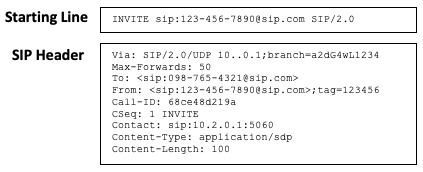
\includegraphics[width=0.7\columnwidth]{chapters/3/img/SIPpacket.png}
    \caption{Example SIP packet}
    \label{f:sippacket}
  \end{center}
\end{figure}


Creating regular expressions for content filtering or pattern matching  is a complex problem that often requires subject matter expertise and manual intervention. Cross-examining multiple packet payloads and examining technical reference documents like RFCs is a time-consuming but necessary process to derive accurate and effective regular expressions. Furthermore, these signatures must be regularly maintained, tested, and updated. Regular expressions become immediately ineffective for example if version numbers are added or changed. In the cybersecurity domain, malware signatures may be easily subverted through simple code or string manipulation so permutations must also be considered. In order to expedite this process and increase signature scope, researchers have leveraged knowledge discovery techniques and applied data mining to extract common features from packet payloads and header contents as input into regular expression signature generation algorithms.

We designed \textsc{Rexactor}, a \textbf{R}egular \textbf{EX}pression \textbf{A}priori \textbf{C}onstruc\textbf{TOR} to extend the state-of-the-art and create more expressive signatures than other solutions are previously capable of generating. \textsc{Rexactor} uses techniques from bioinformatics and natural language processing to encode signatures which use more regex characters and capture more data than previous work while reducing the dynamic memory footprint when employed in regular expression scanning solutions.

\section{Previous Work}

Applications for regular expression signature matching to packet payloads originate in content inspection for malware detection. Early work in automatic signature generation for polymorphic worms such as Autograph \cite{KimHyangAh} provided a foundation for signature-based analysis. This expanded into detecting personally identifiable information as well as policy violations such as copyright infringement, inappropriate or sensitive information on enterprise networks, and censorship~\cite{}. Additionally, Tang et al \cite{TANG2009827} found multiple sequence alignment to be effective in rewarding consecutive substring extractions and tolerating noise in traffic. SigBox~\cite{Shim2017SigBoxAS} introduced the technique of generating substring tokens from packet payloads and applying Apriori data mining to find the most frequent ones. The related CSP Algorithm \cite{Sija} and works by Wang et al \cite{WANG2012992}, Szabo et al \cite{Szabo}, LASER \cite{LASER}, and AutoSig \cite{AutoSig} all include feature extraction and sequence alignment. Wang et al describe their system as a four-stage process; we generalize this concept to all these solutions and our own in order to compare various approaches.

In the first step, data is pre-processed in order to prepare it for use at the next stage. This typically involves extraction of certain fields or N number of bytes from the packet payload. For all these systems, sessionization of packet flows and sometimes defragmentation and reassembly based on TCP/IP header values is required \cite{Shim2017SigBoxAS, WANG2012992, Sija, Szabo, AutoSig, LASER}. Once the data is collected and prepared, the second stage finds common substrings across packet data and/or protocol flows. The systems examined which perform feature extraction use either a subtree approach \cite{WANG2012992}, a longest common substring algorithm \cite{AutoSig, LASER}, motifs \cite{Szabo}, or sequential pattern mining \cite{Shim2017SigBoxAS, Sija}. Third, a method of alignment is used to align data based on commonalities between packets. Wang et al, Szabo et al, Vinoth et al \cite{VinothGeorge2013EfficientRE} and LASER use bioinformatics approaches to perform these alignments. A substring tree can also be used for this purpose \cite{AutoSig}. Some of these alignment strategies are additionally informed by a scoring matrix influenced by the tokens derived in the previous step \cite{WANG2012992, Szabo, LASER}. Once the sequences are aligned in an optimal manner, in the fourth and final stage the systems convert their results into regular expressions.

\section{Methodology}
We use a modified version of Apriori algorithm combined with frequency position tables in order to calculate single byte-length tokens and frequently occurring substrings using choice operators and position constraints \cite{WANG2012992}. \textsc{Rexactor} also uses genetic sequence alignment to find commonalities in payloads and encodes this alignment in order to create a regular expression from it. Our system performs better than previous work in memory space allocation by additionally using position frequencies to specify character classes and length constraints instead of generic wildcards. This creates real-time performance optimization in the scanner. Furthermore, unlike previous solutions our system requires no packet buffering or traffic flow information to do its identification.

\textsc{Rexactor} is made up of component modules which perform various stages of data processing and analysis in order to create optimal regular expressions. The flow of the system is shown in Figure~\ref{f:diagram}. \textsc{Rexactor} takes in as input packet capture (PCAP) files and extracts session payload strings for supported protocols. The input can be of any mix of traffic types, and is therefore well-suited to learning in the wild from real network captures. This extraction layer takes in parameters from the command line interface to select a supported protocol and message type to specifically isolate training data from the mixed input. It also offers an extraction option for the full data layer for analysis. For our experiments, we selected HTTP, SIP, and RTSP as protocols and extracted request and response session payloads for each of them.

\begin{figure}[hbt!]
  \begin{center}
    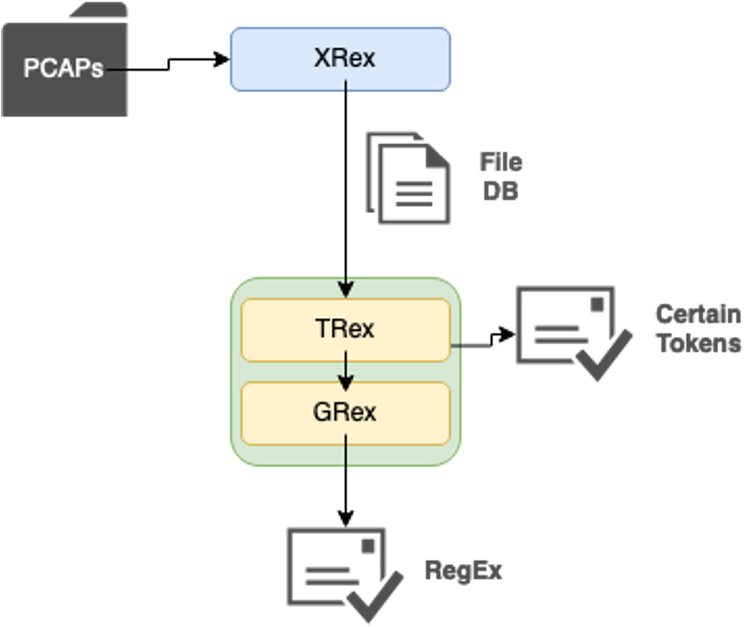
\includegraphics[width=0.6\columnwidth]{chapters/3/img/diagram.png}
    \caption{High-level diagram of signature construction in \textsc{Rexactor}. The system produces certain tokens and regular expressions which can be used with the HRex Scanner or any external filtering/sniffing application.}
    \label{f:diagram}
  \end{center}
\end{figure}

\subsection{TRex: Apriori Tokenization of Packet Payloads}
Inside the starting lines, some substrings appear frequently across packets and thus can be used as string literals in signatures. In the SIP protocol, the line ``\texttt{SIP/2.0}'' appears at the end of all starting lines in all our training data SIP requests. In HTTP, the protocol name and version ``\texttt{HTTP/1.1}'' appear consistently, as well. We use a modified version of the Apriori Algorithm \cite{Toivonen2017} in order to find frequently occurring substrings, or \textit{tokens}, in our packet strings. Shim et al also use Apriori in SigBox for content strings \cite{sigbox}.

Apriori is an algorithm used for finding frequent item sets and association rules from databases. The algorithm uses a bottom-up approach to combine items into incrementally larger item sets, keeping only those sets which meet some minimum threshold of support. The support of an itemset in the database is defined as the number of instances of the itemset in the transactions over the total number of transactions \cite{Toivonen2017}.

\vspace{\baselineskip}

\[\text{Support(X)} = \frac{\text{Instances of X in transactions}}{\text{Number of transactions}}\] \par

\vspace{\baselineskip}

In the formal definition provided by Rakesh Agrawal \cite{Agrawal}, let $I = \{i_{1},i_{2},i_{3}...i_{n}\}$ be a set of items of length \textit{n} and $D = \{t_{1},t_{2},t_{3}...t_{n}\}$ be the set of transactions known as a database. Every transaction $t_{i}$ has a unique identifier in $D$ and $\forall t_{i} : x \in t_{i} \rightarrow x \in I$, or every transaction is a subset of items in $I$. Apriori relies on the anti-monotonicity of the support of itemsets which assumes that all subsets of a frequent itemset must also be frequent, and all supersets of an infrequent itemset must also be infrequent. \par

\begin{algorithm}
\SetAlgoLined
\KwResult{Frequent Itemsets}
 $k=1$, $I_{k} = \{\text{frequent item sets of size 1}\}$\;
 \While{\text{(}$I_{k} \neq \emptyset$\text{)}} {
 $C_{k+1} = apriori\_gen(I_{k})$\;
 \For{$t \in D$} {
      $C_{t} = subset\text{(}C_{k+1}, t\text{)}$\;
      \For{$c \in C_{t}$} {
      c.count++\;
      }
      $I_{k+1} = c \in C_{k+1} \text{ }\vert \text{ } c.count \geq minsup$\;
   }
   $k = k + 1$\;
  }
  $\text{tokens} = \cup_{k}I_{k}$\;
  \Return $\text{prune\_substrings(tokens)}$\;
 \caption{Modified Apriori Algorithm \cite{Agrawal}}
\end{algorithm}

We mine tokens using a modified Apriori approach. Each packet string derived from pre-processing is treated as an individual line in the database. TRex uses a sliding window algorithm of length $k$ to create substring items which are grouped into a list treated as a single transaction. We initialize the window size to $k=2$ in order to prevent likely frequent but meaningless single-byte tokens and set the maximum itemset length $l=1$. The first iteration calculates the frequency of substrings of length $k=2$ and each subsequent loop increments $k$ until no more frequent itemsets (substrings) are found.

Because the order of substrings matters in regular expression matching, we limit the maximum itemset length to 1. We increase item size instead by increasing the window size, thereby preserving order of characters in the modified algorithm. At each iteration, we also prune the resulting token set by replacing tokens $i$ in the current set $S = \{I_{k_{0}}, I_{k_{1}}, I_{k_{2}}...I_{k_{n}}\}$ with any strings $j$ in the result set $I_{k_{n+1}}$ which are superstrings of $i$ and $ support\text{(i)} = support\text{(j)}$. This reduces redundancy of tokens such as ``SIP'' and ``SIP/'' when the sets are unioned together.

\begin{figure}[hbt!]
  \begin{center}
    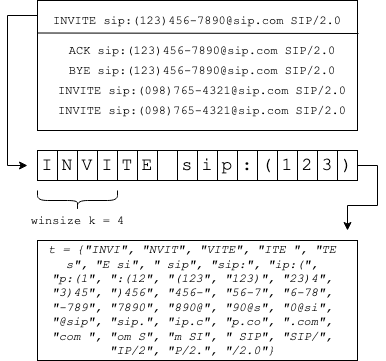
\includegraphics[width=0.7\columnwidth]{chapters/3/img/slidingwindow.png}
    \caption{Modified Apriori Algorithm for string packet data using a sliding window algorithm. The sliding window process is repeated for all packet strings in the database file to make the full set of transactions.}
    \label{f:slidingwindow}
  \end{center}
\end{figure}

\textit{Certain tokens}. Substrings with support equal to 1.0. \par
\textit{Frequent tokens}. Substrings with support equal to a manually configured threshold. For example, in SIP 2.0 the method words \texttt{INVITE}, \texttt{ACK}, and \texttt{BYE} frequently occur in request packets. \par

In order to give positional context to tokens, we introduce position frequency tables from natural language processing (NLP). This allows TRex to compute prefix and suffix groups from frequent tokens. Given a list of tokens $t_{1}, t_{2}, t_{3},...t_{n}$, TRex constructs a position frequency table for each token in each starting line in the database. The resulting vector $V=[\{ t_{1}:pos_{1}, t_{2}:pos_{2}, t_{3}:pos_{3},...t_{n}:pos_{n}\}, \{ t_{1}:pos_{1}, t_{2}:pos_{2}, t_{3}:pos_{3},...t_{n}:pos_{n}\}...]$ is referenced for tokens which occur at $pos=0$. If the sum of support for those tokens found at $pos=0$ is approximately 1.0 with respect to a minimal noise threshold, all tokens in this subset are captured in a prefix group. In the SIP request example, the methods \texttt{INVITE}, \texttt{ACK}, and \texttt{BYE} would be captured and separated with regular expression choice operators and a beginning position constraint in the following manner: $\string^\text{(\texttt{INVITE}}\vert\text{\texttt{ACK}}\vert\text{\texttt{BYE}}\text{)}$. \par

For suffixes, TRex uses string manipulation to reverse both the tokens and starting lines, which intuitively reverses the position significance also so that $pos=len(starting\_line)$ is now decides what goes into the capture group. Frequent tokens are reversed back to their original order before being inserted into the suffix, and choice operators and an end position constraint are appended. Example suffixes may include response codes, status codes or messages, or version numbers of protocols. An example output from TRex configured for HTTP requests and run on data containing both v. 1.0 and v. 1.1 requests may derive a suffix such as $\text{(\texttt{HTTP/1.0}}\vert\text{\texttt{HTTP/1.1}}\text{)\$}$.

In addition to forming prefixes and suffixes, position frequency tables also give meaning to single-byte tokens which occur with $freq=1.0$ at a fixed position. Wang et al found that some protocols have distinctive features at fixed offsets. As an example, they showed that the QQ messaging application always ends its packets with the byte \texttt{0x03}, indicating the end of a message \cite{WANG2012992}. We calculate position frequency tables similar to their approach for each character in each starting line and repeat the process in reverse in order to find single-byte tokens. These tokens are then added to the certain tokens set for future regular expression insertion. The substring tokens are then extracted from the relevant database lines and the remainder is preserved for the alignment stage.

\subsection{GRex: Genetic Sequence Alignment of Common Substrings}

GRex uses principles from genetic sequencing algorithms in order to pairwise align the remaining starting line data. Because we pre-process data into starting lines and TRex removes the found prefixes and suffixes to concentrate on only data which should be aligned, it is appropriate in our system to use a global alignment algorithm which attempts to align the entire sequence pair. We also use progressive alignment to sequentially align pairwise sequences to derive a resulting optimal alignment.

We chose to utilize the Needleman-Wunsch Algorithm for scoring and global alignment \cite{NEEDLEMAN1970443}. As a dynamic programming algorithm, Needleman-Wunsch utilizes a 2D scoring matrix which rewards matching characters and penalizes mismatches according to predefined parameters. Furthermore, a gap penalty is introduced to account for insertions/deletions (indels) in the string alignment. The principle of the algorithm is to greedily maximize the score of alignment per cell. Each cell in the matrix also contains a pointer value which points to the origin of the highest score and will aid in the final trace-back stage \cite{blast}. The score function $F$ with gap score $g$, sequence $A = \{a_{1}, a_{2}, a_{3},...a_{n}\}$, and sequence $B = \{b_{1}, b_{2}, b_{3},...b_{k}\}$ is defined as follows:\par

\begin{equation}
  F(i,j) = max
    \begin{cases}
    F(i-1, j-1) + score(a_{i}, b_{j}) \\
    F(i-1, j) + g \\
    F(i, j-1) + g \\
    \end{cases}
\end{equation}
\vspace{\baselineskip}

In the initialization phase, the first row and column are set as the gap score times the distance from the origin, which is the upper left most corner of the matrix. From here, the algorithm recursively computes the match score, horizontal gap score, and vertical gap score for each cell in the matrix. The match score is calculated from the preceding diagonal cell's score and the score of alignment of the two characters (match or mismatch). The horizontal gap score is the sum of the score to the left and the and the gap score. Similarly, the vertical gap score is the sum of the cell above and the gap score. The cell is set to the maximum of these values and the pointer to the cell (left, vertical, or diagonal) where the maximum came from. Once the matrix has been filled, the pointers are used to trace back through to find the highest-scoring alignment \cite{blast}. Figure \ref{f:needlemanwunsch} demonstrates this scoring algorithm in a matrix.

\begin{figure}[hbt!]
  \begin{center}
    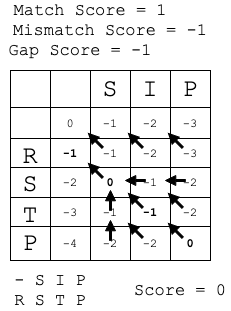
\includegraphics[width=0.3\columnwidth]{chapters/3/img/needlemanwunsch.png}
    \caption{Scoring matrix example of the Needleman-Wunsch Algorithm. Traceback follows from the right bottom corner to the top left cell. The alignment results in the maximum possible score = 0.}
    \label{f:needlemanwunsch}
  \end{center}
\end{figure}

GRex modifies the Needleman-Wunsch algorithm to encode Greek symbols into our alignments which represent specific character classes, insertions and deletions, and mismatches which will later be decoded in the final translation step and used to generate regular expressions. Table \ref{table:greekencoding} provides a key to GRex's Greek symbol encoding. Previous work used an encoding algorithm for indels and mismatches \cite{WANG2012992}, but we created our own encoding schema for GRex and expanded this to also incorporate defining character classes. Specifically, we encode symbols based on whether a character in a given position is or is not a white space character, alphabet character, or digit. Table \ref{table:regexes} shows the regular expression operators GRex derives from these encodings at the translation step.

\begin{table}
\begin{center}
\begin{tabular}{|c | l|}
  \hline
  $\Phi$ & insertion/deletion \\
  \hline
  $\Delta$ & mismatch \\
  \hline
  $\psi$ & gap \\
  \hline
  $\Sigma$ & alphabet character \\
  \hline
  $\omega$ & not alphabet character\\
  \hline
  $\Pi$ & digit \\
  \hline
  $\lambda$ & not digit \\
  \hline
  $\Omega$ & white space character \\
  \hline
  $\sigma$ & not white space character \\
  \hline
\end{tabular}
\caption{Greek Symbols For GRex Encoding}
\label{table:greekencoding}
\end{center}
\end{table}

\begin{table}
\begin{center}
\begin{tabular}{|c|c|p{0.5\linewidth}|}
  \hline
  Type & Symbol & Definition \\
  \hline
  & $.$ & matches any character \\
  \cline{2-3}
  & [] & matches any character in brackets \\
  \cline{2-3}
  & [$\string^$] & matches any character not in brackets \\
  \cline{2-3}
  & \textbackslash s & white space character \\
  \cline{2-3}
  character class & \textbackslash d & digit \\
  \cline{2-3}
  & \textbackslash w & word character \\
  \cline{2-3}
  & \textbackslash S & not white space character \\
  \cline{2-3}
  & \textbackslash D & not digit \\
  \cline{2-3}
  & \textbackslash W & not word character \\
  \hline
  & * & matches zero or more times \\
  \cline{2-3}
  & ? & matches at most one time \\
  \cline{2-3}
  quantifier & + & matches one or more times \\ \cline{2-3}
  & \{$m,n$\} & matches between $m$ and $n$ times \\
  \cline{2-3}
  & \{$m$,\} & matches $m$ or more times \\
  \cline{2-3}
  & \{,$n$\} & matches at most $n$ times \\
  \hline
  & $\string^$ & matches beginning of data \\
  \cline{2-3}
  other & \$ & matches end of data \\
  \cline{2-3}
  & () & capture group \\
  \cline{2-3}
  & $\vert$ & OR operator \\
  \hline
\end{tabular}
\caption{Supported Regular Expression Operators}
\label{table:regexes}
\end{center}
\end{table}

The encoding process runs in a progressive manner, such that two strings are aligned, compared, and encoded, and that return is then passed again and compared against another string in the sequence. Once aligned using the Needleman-Wunsch algorithm, the character types of each index are compared. Depending on the type of character, the returned string from this process is appended with a representation of either the character itself if the indexes are matching or a Greek character encoding otherwise. Once the new string is fully appended, it is returned to the loop. This returned string is compared to the next entry within the data. This process loops until every line from the packet data is aligned into the final encoding.

In order to create the regular expression, the replacement function is run against the generated string. Each index is checked and replaced with the regular expression counterpart with correct special character escaping. The final regular expression is constructed from the symbolic string. Frequent tokens are combined with choice operators and positional constraints $\string^$ and $\$$ for prefixes and suffixes, respectively. Prefixes are appended to the beginning of the generated regular expression, and suffixes to the end.

\subsection{HRex: High Performance Regular Expression Scanning}
The final component is a sniffing application written in C++ which reads in PCAP files using \texttt{libpcap} and performs regular expression scanning with Intel's Hyperscan library~\cite{hyperscan}. Hyperscan provides significant performance improvement over other commercial but popular tools like Snort due to its reduction of duplicate operations in string and pattern matching and use of single-instruction, multiple data (SIMD) operations. In their experimentation, creators of Hyperscan found it outperformed Snort by a factor of 8.7~\cite{hyperscanusinex}. Our string literal tokens created by \textsc{Rexactor}'s TRex can be applied in a pre-filter system like Snort, as well. Furthermore, Hyperscan does additionally support string literal, or keyword, matching. We provide both solutions for flexibility in real-world applications as the network capture environment is rarely one-size-fits-all. As our tokens are learned via unsupervised learning, they do not require manual analysis and thus scale well to larger, unknown data sets.

\section{Experiments and Results}

We performed two case studies using \textsc{Rexactor} regular expressions and tokens. The first is a comparison-based analysis using our own HTTP signature and ones developed by related works. Additionally, we assessed \textsc{Rexactor}'s ability to develop a signature and keywords for SIP and RTSP, two protocols found in VoIP traffic flows. We use measures of precision, recall, and F1 score in order to assess signature efficacy.

We use measures of precision, recall, and F1 score in order to assess signature efficacy. Our measure of recall is the number of packets $n$ correctly identified as protocol type $P$ divided by the sum of the number of packets $n$ correctly identified by their protocol type plus the number of packets $m$ incorrectly identified as not $P$ \cite{Zhang}.

\vspace{\baselineskip}
\[\text{Recall} = \frac{\text{$n$ correctly labeled $P$}}{\text{$n$ correctly labeled $P$ + $m$ incorrectly labeled not $P$}}\] \par
\vspace{\baselineskip}

Precision is defined as the number of packets $n$ correctly identified as protocol type $P$ divided by the sum of the number of packets $n$ correctly identified as protocol type $P$ plus the number of packets $m$ incorrectly identified as $P$ \cite{Zhang}.

\vspace{\baselineskip}
\[\text{Precision} = \frac{\text{$n$ correctly labeled $P$}}{\text{$n$ correctly labeled $P$ + $m$ incorrectly labeled $P$}}\] \par
\vspace{\baselineskip}

Finally, we also provide the F1 score for ours and other solutions.

\vspace{\baselineskip}
\[\text{F1} = 2 \times \frac{\text{Precision $\times$ Recall}}{\text{Precision + Recall}}\] \par
\vspace{\baselineskip}

In addition to these data science measurements, we record, analyze, and compare heap usage using \texttt{valgrind}. We also compare the heap allocation for our signatures and signatures from comparable works to show our solution's improvements.

We use packet capture (PCAP) data from live network captures for both training and testing scenarios. An interesting note on training data is that in our cases, \textsc{Rexactor} did not require more than a few hundred starting lines in order to create quality signatures. We found that as long as the starting lines were from a diverse set of captures so that variable URLs, ports, and addresses were not over-represented, the common features were both discovered and generalized enough for re-usability. This demonstrates that \textsc{Rexactor} may be able to create specific signatures for protocols which may not appear frequently in a data set.

To create HTTP signatures with \textsc{Rexactor}, we used a small data set of mixed background traffic containing 213 HTTP request packets and 1000 HTTP responses. The resulting signatures and tokens are provided in Table \ref{table:http}. For the VoIP protocol tests, we used 252 SIP request packets and 230 responses for training signatures, and 638 RTSP responses and 562 RTSP requests. Our signatures and tokens for these are provided in Table \ref{table:voip}. We ran tests on data sets from a live capture environment of background web traffic containing 1000 HTTP packets, 1000 SIP packets, 1000 RTSP packets, and 1000 packets of other mixed protocol types, including FTP, SMTP, ICMP, and others.

\textsc{Rexactor} is a Python tool library designed with Python 3.8. We use the efficient-apriori library (v. 1.1.1) \cite{efficient-apriori} for tokenization, PyShark for data pre-processing (v. 0.4.3) \cite{pyshark}, and numpy (v. 1.21) \cite{numpy} data structures for optimization.  The scanning framework used for testing regular expression matching is written in C++ using Boost 1.63 \cite{boost} and Hyperscan 5.4.0 \cite{hyperscan} libraries for regular expression creation and matching, respectively. All experiments were performed on a single i9 Dell computer with Ubuntu 20.04 installed.

\subsection{Case Study A: HTTP Detection}

\begin{table*}[t]
  \centering
  \begin{tabular}{|p{0.12\linewidth}|l|p{0.3\linewidth}|p{0.3\linewidth}|}
 \hline
 Source & Side & Signatures & Tokens \\ [0.5ex]
 \hline\hline
 AutoSig \cite{AutoSig} & N/A & N/A & [HTTP/1.]; [GET\textbackslash0x20/] [HTTP/1.];\\
 \hline
 LASER \cite{LASER} & N/A & N/A & [HTTP/1.1] \\
 \hline
 Wang et al \cite{WANG2012992} & Request & $\string^$(GET $\vert$ HEAD $\vert$ POST).*HTTP/1.(1$\vert$0) \textbackslash x0D\textbackslash x0A & N/A\\
 \cline{2-4}
  & Response & $\string^$HTTP/1.(1$\vert$0) [2$\vert$3$\vert$4$\vert$5]0.*\textbackslash x0D\textbackslash x0A & N/A \\
 \hline
 LCS Algorithm \cite{VinothGeorge2013EfficientRE} & N/A & $\string^$(HTTP/1.1 $\vert$ Host:.u $\vert$ Connection:keep-alive $\vert$ User-Agent:Mozilla/5.0 $\vert$ Accept: $\vert$ Accept-Encoding:ga $\vert$ Accept-Language:en-US.*en;q=0.8 $\vert$ Accept-Charset:ISO-8859-1)  & [HTTP/1.1]; [Host:.u]; [Connection:keep-alive]; [User-Agent:Mozilla/5.0]; [Accept:]; [Accept-Encoding:ga]; [Accept-Language:en-US.*en;q=0.8]; [Accept-Charset:ISO-8859-1]\\
 \hline
 \textsc{Rexactor} & Request & $\string^$(GET / $\vert$ POST / $\vert$ POST $\vert$ POST /mail $\vert$ HEAD /).\{0,2048\}( HTTP/1.1\textbackslash r\textbackslash n)\$ & [HTTP/1.]\\
 \cline{2-4}
 & Response & $\string^$(HTTP/1.1 $\vert$HTTP/1.).\{0,3\}.\{0,24\} \textbackslash\textbackslash S(\textbackslash r\textbackslash n)\$ & [HTTP/1.] \\ [1ex]
 \hline
  \end{tabular}
  \caption{HTTP Signatures and Tokens}
  \label{table:http}
\end{table*}

The results of scanning related works' regular expressions and our own on the testing dataset showed comparable recall for Wang et al's system and \textsc{Rexactor}. The longest common substring algorithm (LCS) signature performed significantly worse. For our dataset, all systems for both regular expression scanning and literal token scanning had perfect precision, including \textsc{Rexactor}. Because precision in our data set was ideal for all systems, the F1 Score results are comparable to the recall results.

While precision and recall results were on par with the state-of-the art, \textsc{Rexactor}'s signature required significantly less heap space than either Wang et al's solution or LCS when performing regular expression scanning. This demonstrates \textsc{Rexactor}'s superior performance in real embedded systems where memory optimization is a critical factor.

\begin{table}[H]
  \centering
  \begin{tabular}{|l|l|l|l|l|}
   \hline
   Solution & P & R & F1 & Allocation \\
   \hline\hline
   Wang et al & 1.000 & 0.984 & 0.992 & 20,783,011 bytes\\
   LCS & 1.000 & 0.254 & 0.405 & 36,015,510 bytes \\
   \textsc{Rexactor} & 1.000 & 0.976 & 0.989 & 18,310,656 bytes\\

   \hline
  \end{tabular}
  \caption{HTTP Case Study Results for Regular Expressions}
  \label{table:httpprecisionregex}
\end{table}

\begin{table}[H]
  \centering
  \begin{tabular}{|l|l|l|l|l|}
   \hline
   Solution & P & R & F1 & Allocation \\
   \hline\hline
   AutoSig & 1.000 & 0.989 & 0.994 & 548,715 bytes \\
   LASER & 1.000 & 0.865 & 0.928 & 457,778 bytes \\
   \textsc{Rexactor} & 1.000 & 0.989 & 0.994 & 457,280 bytes \\
   \hline
  \end{tabular}
  \caption{HTTP Case Study Results for Tokens}
  \label{table:httpprecisiontokens}
\end{table}

\subsection{Case Study B: VoIP Detection}
\begin{table*}[t]
  \centering
  \begin{tabular}{|p{0.12\linewidth}|l|p{0.3\linewidth}|p{0.3\linewidth}|}
   \hline
   Protocol & Side & Signatures & Tokens \\ [0.5ex]
   \hline\hline
   SIP & Request & $\string^$(INVITE sip:$\vert$ACK sip:$\vert$BYE sip:$\vert$REGISTER sip:).\{0,74\}( SIP/2.0)\$ & [ sip:];[ SIP/2.0] \\
   \cline{2-4}
   & Response & $\string^$(SIP/2.0 200 OK$\vert$SIP/2.0 40$\vert$SIP/2.0 100 Trying$\vert$SIP/2.0 180 Ringing$\vert$SIP/2.0 4$\vert$SIP/2.0 18$\vert$SIP/2.0 ).\{0,31\} & [SIP/2.0 ] \\
  \hline
  RTSP & Request & $\string^$(TEARDOWN rtsp://$\vert$DESCRIBE rtsp://$\vert$SETUP rtsp://$\vert$PLAY rtsp://).\{0,85\}( RTSP/1.0\textbackslash r\textbackslash n)\$ & [rtsp://];[RTSP/1.0\textbackslash r\textbackslash n] \\
  \cline{2-4}
  & Response & $\string^$(RTSP/1.0 )\textbackslash\textbackslash d\textbackslash\textbackslash d\textbackslash\textbackslash d .\{0,6\}[a-zA-Z](\textbackslash r\textbackslash n)\$ & [RTSP/1.0 ] \\
  \hline
  \end{tabular}
  \caption{VoIP Signatures and Tokens}
  \label{table:voip}
\end{table*}

In addition to a comparison study using HTTP, we ran precision, recall, and memory allocation tests for \textsc{Rexactor} signatures for two VoIP protocols. In future work, we could expand this to chat, email, and other text-based protocols with the goal of targeting signatures for application-specific signature generation and protocol analysis. For example, we would want to target identifying and distinguishing between Skype, Zoom, or Webex traffic flows \cite{Zhang}. \textsc{Rexactor} performed amicably with perfect recall and precision in our dataset. Heap allocation results were also comparable to HTTP, showing that the good performance from the case study was not anomalous but rather indicative of good signature construction by \textsc{Rexactor}.

\begin{table}[H]
  \centering
  \begin{tabular}{|l|l|l|l|l|}
   \hline
   Protocol & P & R & F1 & Allocation \\
   \hline\hline
   SIP & 1.000 & 1.000 & 1.000 & 34,449,057 bytes\\
   RTSP & 1.000 & 1.000 & 1.000 & 14,972,715 bytes \\
   \hline
  \end{tabular}
  \caption{VoIP Results for Regular Expressions}
  \label{table:voipregex}
\end{table}

\begin{table}[H]
  \centering
  \begin{tabular}{|l|l|l|l|l|}
   \hline
   Protocol & P & R & F1 & Allocation \\
   \hline\hline
   SIP & 1.000 & 1.000 & 1.000 & 3,234,815 bytes\\
   RTSP & 1.000 & 1.000 & 1.000 & 3,624,176 bytes \\
   \hline
  \end{tabular}
  \caption{VoIP Results for Tokens}
  \label{table:voiptokens}
\end{table}

RExACtor provides a classification solution for per-packet analysis and does not require data to be read as or reconstructed into flows in order to achieve classification. The modular design of RExACtor also allows for components to be used as tool sets so that engineers may adapt the knowledge discovery elements to their own scanning systems or use the full system as a whole framework. For example, the module TRex which derives tokens may be run individually in order to create keywords for Snort filters. Additionally, regular expression signatures can be created and published outside of the scanner in order to be plugged into any other DPI application. RExACtor also supports tokenization and alignment for raw data, allowing for analysis and signature creation for unknown protocols. This high adaptability means RExACtor can be applied in many network environments for knowledge discovery and DPI usage.
Currently, RExACtor supports email (SMTP, POP3, IMAP), file transfer (FTP), chat (XMP, IRC), VoIP (SIP, RTSP), and web (HTTP) protocol analysis. Because RExACtor utilizes unsupervised learning and derives features from training data, it could be applied to learning more application specific signatures. One improvement for our solution and others discussed which use unsupervised learning would be an attempt to learn an optimal threshold for feature support rather than rely on manual configuration. In the comparison study, we found that packets not identified by the signatures were HTTP continuation packets of just data payload. Sessionization of protocol flows would allow a detection system to pick up on the first HTTP packet of an exchange with identifying method information, then record the 5-tuple flow information for further scanning. But this technique is not usable in per-packet analysis, and is a limitation of the problem space rather than our solution.

Regular expressions as a text-based approach also have limitations to their applicability in the real, complex network environment. The current industry standard for application layer DPI is to use regular expressions to match expected values in payloads. Protocols or applications may have multiple signatures to match request, response, or message types. Some protocols also do not have strong signatures. Furthermore, different versions of protocols or updated standards and RFCs often require separate signature sets and the continual update of older patterns~\cite{rexactor}. Some protocols are also so non-standard that it is difficult to track them on a regular expression signature alone; for example, the payload of an RTP packet is raw data and assigned ports are dynamic~\cite{rfc3550}. Current state-of-the-art scanners suffer from variable and data-dependent performance impact~\cite{deepmatch}. With the increasing size and complexity of rulesets and the growing scale of the network environment, regular expression scanning using the current systems is more and more impractical. Regex methods are also limited by what classes they can be used for in network traffic. For example, there is no real regular expression signature which can identify Tor-routed traffic from non-Tor-routed traffic; the data is too diverse. Other desirable classes for traffic, such as traffic type, application, and user or device type present similar issues to regular expression scanners. Each possiblity must have its own, human-engineered regular expression to match precisely which is both slow and prone to error. In addition to scalability and machine performance, text-based regular expression matching no longer meets the needs of the environment as over 90\% of browsing data today is encrypted~\cite{google}.

Regular expression matching which relies on deterministic and non-deterministic finite automata (DFA and NFA) is prone to the state explosion problem, where computational complexity increases exponentially as regular expressions increase in number and  become more complex. DFAs are fast to search, but are most prone to state explosion as every possibility is explicitly constructed. NFAs provide linear storage space to the size of the regular expression ruleset, but it is relatively easy to arrive at worst-case search performance with rule complexity~\cite{alpinepalm}. ~\cite{Fu}. Table~\ref{table:facomplex} shows the processing complexity and storage costs of these structures where $m$ is a number of regular expressions of length $n$.

\begin{table} [ht!]
\caption{Worst-Case Space and Time Complexities for NFA and DFA~\cite{Yu}}
\centering
\begin{tabular}{|c | c | c|}
\hline
\textbf{Data Structure} & \textbf{Complexity} & \textbf{Storage Cost} \\
\hline
NFA & $O(n^{2}m)$ & $O(nm)$ \\
\hline
DFA & $O(1)$ & $O(\Sigma^{nm})$ \\
\hline
\end{tabular}
\label{table:facomplex}
\end{table}

Recently, hybrid NFA/DFA engines have been proposed to improve search performance; however, improvements on computational complexity can still be prone to memory issues in the case of large regular expression rulesets~\cite{hyperscan}. Parallel computing may alleviate some of the computational stress, but is acknowledged as a brute force approach~\cite{Fu}. Hyperscan is able to handle compiling and searching with incredible efficiency; however, this becomes exponentially worse to the point of impracticality when put at a test to scale, which we demonstrate in the next chapter of this work.


\chapter{ALPINE/PALM - SIMILARITY SEARCH THROUGH LOCALITY-SENSITIVE HASH FINGERPRINTING}
\section{Introduction}
The ineffectiveness of existing regular expression DPI methods against encrypted payloads and weakly signatured data classes as well as the computational and storage complexity of automata has caused researchers to shift to other forms of traffic fingerprinting for identification. We propose using locality-sensitive hashing in order to measure similarity of features between packets. Locality-sensitive hashing uses a distance metric to preserve the similarity of original inputs when they are converted to locality-sensitive hashes (LSH). The benefit of locality-sensitive hashing here is that it is capable of reducing high-dimensionality data into a low-dimensional, space-effective, computationally efficient representation of the same data while still preserving similarity metrics between the data points~\cite{jafari2021survey}. Hash families may be defined for many distance measures such as Hamming distance, L1 and L2 norm~\cite{ANN-CoD}, and Jaccard similarity~\cite{minhash}.

Contrary to cryptographic hashes which attempt to avoid collision, locality-sensitive hashes preserve the similarity of data points (in our case, token sets) to one another. The following definition intuitively states that data points which are locally nearby have a higher probability of collision than further points.

\medskip

\begin{definition}
\textit{~\cite{lshforest} A family $H$ of functions from a domain $S$ to a range $U$ is called ($r$, $\epsilon$, $p_1$, $p_2$)-sensitive, with $r$, $\epsilon > 0$, $p_1 > 0$, $p_2 > 0$, if for any $p$, $q \in S$, the following conditions hold:}
\begin{itemize}
\item{\textit{if $D(p, q) \leq r$ then $Pr_H[h(p) = h(q)] \geq p_1$,}}
\item{\textit{if $D(p, q) > r(1 + \epsilon)$ then $Pr_H[h(p) = h(q)] \leq p_2$.}}
\end{itemize}
\end{definition}

\medskip


One way in which locality-sensitive hashing has been applied in the network security domain is in user-level browser fingerprinting. In this method, web-based browser fingerprints created by extracting multiple values from the browser API may be hashed using MinHash or similar functions to generate signatures of high entropy, where the data is uniquely identifiable as a particular device or host~\cite{browser}. We apply this concept similarly to network packet data, aiming for a locality-sensitive hash using features which should also evidence values unique to the class type. LSH clustering has also been used to create signatures for identifying malware at scale~\cite{bayer}, but has rarely been applied in DPI.

Once hashes are created representative of the packets, differences in the hashes may be compared linearly using a similarity search approximation. Similarity search is a generalized term in data mining which refers to searching for objects where the available comparator is some common pattern or similarities among them. Examples of similarity search mechanisms include Nearest Neighbors searching, link-based similarity searches, duplicate detection, and defining object representations~\cite{lshforest}. Applications for this in the cyber crime space include finding individuals in the same criminal network, finding content online similar to known evidence, querying to find images similar to another, and detecting fingerprints across network data. The best indexes for similarity search have efficient querying and storage mechanisms, minimum memory footprint, and minimal interference required by the developer and maintainer~\cite{simsearch}.

One of the challenges in data engineering is determining how to construct suitable, unique \textit{tokens} which characterize the data meaningfully. The sentence, ``Palm trees are native to the Pacific", may be split on whitespace into the set of tokens $T = \{\text{``palm"}, \text{``trees"}, \text{``are"}, \text{``native"}, \text{``to"}, \text{``the"}, \text{``pacific"}\}$. It is obvious that tokens like \text{``the"} are far too generic in the English language to be characteristic of this sentence, but a token like \text{``palm"} or \text{``pacific"} will be much more unique and indicate a stronger similarity. This idea may be more solidly quantified through taking the inverse document frequency (IDF) of tokens which minimizes the importance of terms which appear frequently in the document set. When combined with term frequency (TF) as the TF-IDF value~\cite{tf-idf}, the most relevant tokens may be found which are both common and characteristically unique of the document set.

\section{Previous Work}

Jaccard similarity measures the intersection of two sets over their union. This value is often used in recommender systems, and can also be used to detect plagiarism or make predictions. In order to take the Jaccard similarity, data must be split up into sets, which are made up of individual elements like the tokens or shingles of strings as done in SigBox~\cite{sigbox} and \textsc{Rexactor}~\cite{rexactor} for regular expression signature generation.

Some limited work has been done in application fingerprinting through locality-sensitive hashing. Tang et al proposed HSLF~\cite{hslf}, an HTTP header sequence-based LSH fingerprint generator for classifying applications in HTTP traffic. Their results show the ability of their SimHash-based method to distinguish accurately among data such as VMWare, Firefox, and WeChat. This work is limited as it only applies to cleartext HTTP traffic. Furthermore, the scope of this traffic only makes up a fraction of real-world data.


Jiang and Gokhale~\cite{fpga} use locality-sensitive hashing on packet-level features to accurately classify network traffic statelessly. From a model perspective, their use of K-Nearest Neighbors clustering scales sub-optimally. Their work also focused solely on multimedia applications versus legacy web-browsing; there is no expansion into traffic type, application, protocol, or other needed classification in current DPI. \textsc{Alpine} and \textsc{Palm} expand these works into a much more complex and diverse set of experiments and applications.

\section{Methodology}

\subsection{MinHash and Locality-Sensitive Hash Forest}

In order to form the elements of a set, we \textit{shingle} packets into items and reduce the data to a set intersection problem. An object is $w$-shingled when a sub-sequence of length $w$ of contiguous tokens is cut from it. In \textsc{Alpine}, we use the port information, transport layer protocol, flag values, and packet length to make up our shingles. In \textsc{Palm}, word tokens are created by delimiting packet payloads by whitespace. Thus, each original packet $P$ is now associated with some set $S_P$ of shingles as depicted in Figure~\ref{jacsim}.

\begin{figure} [ht!]
\begin{equation}
J(P_A, P_B) = \frac{|S_A \cap S_B|}{|S_A \cup S_B|}
\end{equation}
\caption{Jaccard Similarity of Shingle Sets}
\label{jacsim}
\end{figure}

Jaccard similarity can be approximated quickly through the MinHash algorithm. The hash representation also fixates and potentially reduces the amount of space packet data occupies, and furthermore normalizes the data in cases where the shingles are heterogenous and of varying length and type. The MinHash of a given column is the number of the first row in permuted order whose characteristic matrix value is $1$. The sequence is continued down the columns and repeated for $k$ permutations. The probability that the MinHash function for a random permutation of rows produces the same value for two sets is a close approximation to their Jaccard similarity~\cite{mmds}. Bawa et al~\cite{lshforest} developed the LSHForest algorithm which indexes the locality-sensitve hashes in a forest-based data structure in order to optimize the similarity search process. It improves upon nearest-neighbor searches by both reducing complexity and eliminating the need to know the distance $r$ from the query to the nearest neighbor of a given data point. Optimization is achieved through the use of a specific set of hash functions which ensures that any nearest neighbor query returns $\epsilon$-approximate neighbors so long as a suitable $l$ number of trees is chosen. LSHForest scales much more efficiently compared to previous work using nearest neighbor searches~\cite{fpga}. The build time of a KNN model can have a complexity of $O(n^2)$, where $n$ is the number of items. In contrast, LSH construction is done in linear time~\cite{lshforest}. The theoretical complexities of operations on LSHForest are provided from the original paper in Table~\ref{table:forestcomplex}. When compared with time and space complexities for the automata in regular expression searching in Table~\ref{table:facomplex}, the logarithmic improvement and fixed storage space is clear. We chose to use this data structure in the classification stage of \textsc{Alpine} and \textsc{Palm} in order to utilize this optimization.

\begin{table} [ht!]
\caption{Time Complexities for LSHForest~\cite{lshforest}}
\centering
\begin{tabular}{|c | c |}
\hline
\textbf{Operation} & \textbf{Complexity} \\
\hline
Insertion & $O(l * log_B n)$ \\
\hline
Deletion & $O(l * log_B n)$ \\
\hline
Query &  $O(l * log_B n) + O(l * log B) + O(M/B)$\\
\hline
\end{tabular}
\label{table:forestcomplex}
\end{table}

In these equations, $l$ represents the number of trees, $n$ the number of data points in the dataset, and $B$ the branching factor of an internal node. Storage is optimized to be linear, $O(n)$, through the use of compressed PATRICIA tries~\cite{lshforest}. The $m$ nearest neighbors for some point $q$ is found by first performing a binary, longest matching prefix search for a leaf node with the point $s_i$. Then some $M$ points are collected synchronously across all trees and ranked by similarity score, with the top $m$ being returned as an answer. The $m$ number is used as votes to classify the sample by majority once the query is complete. This majority vote approach also allows for multiple classification results; for example, an adaptive system may be able to take the second closest result if the first choice turns out to be incorrect.

\subsection{ALPINE: A Locality-Based Packet Inspection Engine}
\textsc{Alpine}~\cite{alpinepalm} is \textbf{A} \textbf{L}ocality-Sensitive \textbf{P}acket \textbf{In}spection \textbf{E}ngine which performs shallow packet inspection on selected features from the network and transport layer encapsulation headers of packets. \textsc{Alpine} uses Jaccard similarity in order to determine likeness between sets of the following packet header features: \textit{source and destination IP address, type of service field, packet length, IP next protocol, IP flags, source and destination port} (see Figure~\ref{fig:alpineheader}). For indexing the computed MinHashes and performing lookup for classification, \textsc{Alpine} uses the previously discussed LSHForest~\cite{lshforest}. A query is performed by computing the MinHash of the input data and doing a binary search on the prefix trees. The hash is then mapped back to its label index. A majority vote is taken from the returned $m$ nearest neighbors and the data is classified accordingly.

\begin{figure} [ht!]
  \centering
  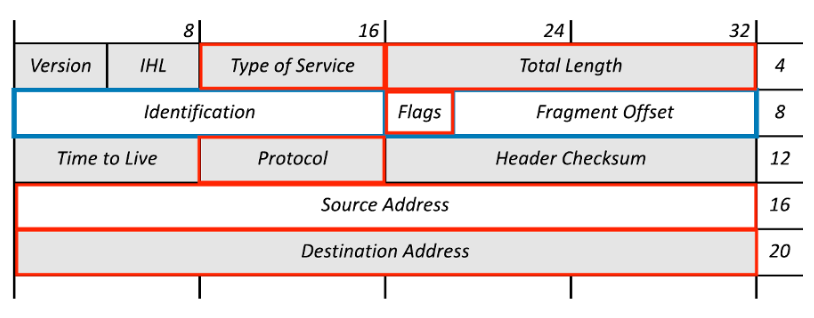
\includegraphics[width=0.8\textwidth]{chapters/4/img/alpineheader.png}
  \caption{Example TCP/IPv4 header with extracted features for \textsc{Alpine} highlighted in red}
  \label{fig:alpineheader}
\end{figure}

\subsection{PALM: Payload Analysis Using Locality Sensitive Measurements}
\textsc{Palm} performs \textbf{P}ayload \textbf{A}nalysis using \textbf{L}ocality-Sensitive \textbf{M}easurements. This is a similar strategy to previous work in payload signature generation like SigBox~\cite{sigbox} and RExACtor~\cite{rexactor}. \textsc{Palm} delimits packet payloads by whitespace in order to create word-style tokens. In future work, other delimiters or a sliding-window shingling technique may suit identification of certain data types such as binary application layer protocols like HTTP2. In the experiments presented in this report, whitespace proved to be the most effective delimiter. We also experiment without using port numbers as identifiers in order to test the possiblity of non-standard port usage and detection. MinHash was used to generate the locality-sensitive hashes for the data samples and test samples. We use the LSHForest algorithm developed by Bawa et al~\cite{lshforest} to index the locality-sensitive hashes and optimize the search process.

\section{Experiments and Results}
\begin{table} [ht!]
\caption{Description of Combined Dataset}
\centering
\begin{tabular}{|c |c | c |}
\hline
\textbf{Application Type} & \textbf{Protocol} & \textbf{\# Samples} \\
\hline
\hline
\textit{File Transfer} & FTP & 10,015 \\
& FTP-DATA & 4,000 \\
& BitTorrent &  20,648 \\
\hline
\hline
\textit{Voice-over-IP} & MGCP & 1,568 \\
& SIP & 1,112 \\
& H.225 &  1,300 \\
& RTP &  15,552 \\
& RTCP &  1,626 \\
\hline
\hline
\textit{Mail} & SMTP & 5,981 \\
& POP & 1,675 \\
& IMAP &  3,318 \\
\hline
\hline
\textit{Authentication \& Access} & LDAP & 1,354 \\
& SMB &  3,554 \\
& Telnet & 1,888 \\
\hline
\hline
\textit{Tunneling} & GPRS & 9,981 \\
& PPTP & 1,288 \\
& SSH & 3,039 \\
\hline
\hline
\textit{Web \& Chat} & DNS & 10,563 \\
& HTTP & 21,298 \\
& XMPP &  1,553 \\
& TLS & 4000 \\
\hline
\hline
\textit{Networking} & DHCP & 1,444 \\
& NBNS & 1,216 \\
& GQUIC &  1,740 \\
& NTP & 1,940 \\
& SSDP &  8,504 \\
\hline
\end{tabular}
\label{table:dataset}
\end{table}

Instead of using a single dataset or network environment to evaluate the system, we used several available public datasets. Our sources include the CDX 2009 captures~\cite{cdx2009}, the Skynet Tor dataset~\cite{skynet}, the Canadian Institute for Cybersecurity's ISCX VPN/non-VPN and Tor/non-Tor datasets~\cite{vpn-dataset, tor-dataset}, and repositories from Wireshark, Cloudshark, and IEEE Dataport. Investigation has shown that using captures from only a single environment can lead to bias in results~\cite{Silva2022}. A machine learning algorithm might learn characteristics of the network or environment such as IP addresses rather than actual protocol features, which can hurt generalizability of the model. For this reason and to increase the scope of classes beyond what is available in any single public dataset, we merged PCAPs from these experiments and created our own repository of twenty-six different, common application layer protocol packet captures. For experimental reproducibility and general use we have made this new dataset available publicly~\footnote{https://github.com/mayakapoor/protocol-dataset}.


\subsection{Protocol Auto Detection}

\begin{table}
\caption{Protocol Autodetection Results}
\centering
\begin{tabular}{| c | p{0.6cm}  p{0.6cm}  p{0.6cm} || p{0.6cm}  p{0.6cm}  p{0.6cm} |}
\hline
& & \textbf{Jaccard} & & & \textbf{TF-IDF} & \\
\hline
\hline
\textbf{Accuracy} & & 0.996 & & & 0.841 & \\
\textbf{Cohen's $\kappa$} & & 0.997 & & & 0.841 & \\
\hline
\hline
 \textbf{Protocol} & \textbf{P} & \textbf{R} & \textbf{F1} & \textbf{P} & \textbf{R} & \textbf{F1} \\
 \hline
 BitTorrent & 1.00 & 0.99 & 0.99 & 0.89 & 0.85 & 0.86 \\
 DHCP & 1.00 & 1.00 & 1.00 & 0.91 & 1.00 & 0.95 \\
 DNS & 1.00 & 0.99 & 1.00 & 0.95 & 0.97 & 0.96 \\
 FTP & 0.99 & 1.00 & 0.99 & 0.83 & 0.90 & 0.86 \\
 FTP-DATA & 1.00 & 1.00 & 1.00 & 0.93 & 0.96 & 0.94 \\
 GPRS & 1.00 & 1.00 & 1.00 & 0.91 & 0.98 & 0.95 \\
 GQUIC & 1.00 & 0.99 & 0.99 & 0.87 & 0.75 & 0.81 \\
 HTTP & 1.00 & 0.99 & 0.99 & 0.82 & 0.48 & 0.61 \\
 H.225 & 1.00 & 1.00 & 1.00 & 0.83 & 0.97 & 0.90 \\
 IMAP & 1.00 & 0.99 & 0.99 & 0.86 & 0.79 & 0.82\\
 LDAP & 1.00 & 0.99 & 0.99 & 0.87 & 1.00 & 0.93 \\
 MGCP & 1.00 & 1.00 & 1.00 & 0.90 & 0.65 & 0.75 \\
 NBNS & 0.99 & 1.00 & 0.99 & 0.94 & 1.00 & 0.97 \\
 NTP & 1.00 & 1.00 & 1.00 & 0.91 & 1.00 & 0.95 \\
 POP & 0.98 & 1.00 & 0.99 & 0.91 & 0.47 & 0.62 \\
 PPTP & 0.95 & 1.00 & 0.98 & 0.84 & 0.90 & 0.87 \\
 RTCP & 1.00 & 1.00 & 1.00 & 0.96 & 1.00 & 0.98 \\
 RTP & 1.00 & 1.00 & 1.00 & 0.89 & 0.88 & 0.89\\
 SIP & 1.00 & 1.00 & 1.00 & 0.54 & 0.98 & 0.69 \\
 SMB & 1.00 & 0.97 & 0.98 & 0.95 & 0.99 & 0.97 \\
 SMTP & 1.00 & 0.99 & 0.99 & 0.92 & 0.93 & 0.93 \\
 SSDP & 1.00 & 1.00 & 1.00 & 0.72 & 0.28 & 0.40 \\
 SSH & 1.00 & 0.98 & 0.99 & 0.90 & 0.86 & 0.88 \\
 Telnet & 0.99 & 1.00 & 0.99 & 0.86 & 0.99 & 0.92 \\
 TLS & 1.00 & 1.00 & 1.00 & 1.00 & 1.00 & 1.00 \\
 XMPP & 1.00 & 1.00 & 1.00 & 0.79 & 0.90 & 0.84 \\
 \hline
\end{tabular}
\label{table:results1}
\end{table}

The autodetection of application-layer protocols is a crucial functionality for lawful interception devices like DPI middleware boxes in order to properly assess, parse, and process the traffic they are checking. The traffic environment on any given signal can be wildly diverse; thus, any classification system must be capable of scaling to a large, multiclass problem. Previous systems~\cite{hslf, fpga} have not attempted protocol detection to the scale of a 26-class problem, making this experiment and our model a true and fresh pioneer in the DPI field. To address the first question, we split the data into training and test sets and extracted the features from each of the protocols. We generated hash values for the training samples, adding them to the classifier. The results of the testing samples are provided in Table~\ref{table:results1}. The evidence shows that the combined model has high accuracy and precision/recall for protocol identifications. Cohen's kappa also shows a strong agreement among the ensemble voters. The method also performs equally well across application types, indicating generalizability. Figure~\ref{fig:combined} shows the confusion matrix results of the classifier's ensemble voting system.

\begin{figure} [ht!]
  \centering
  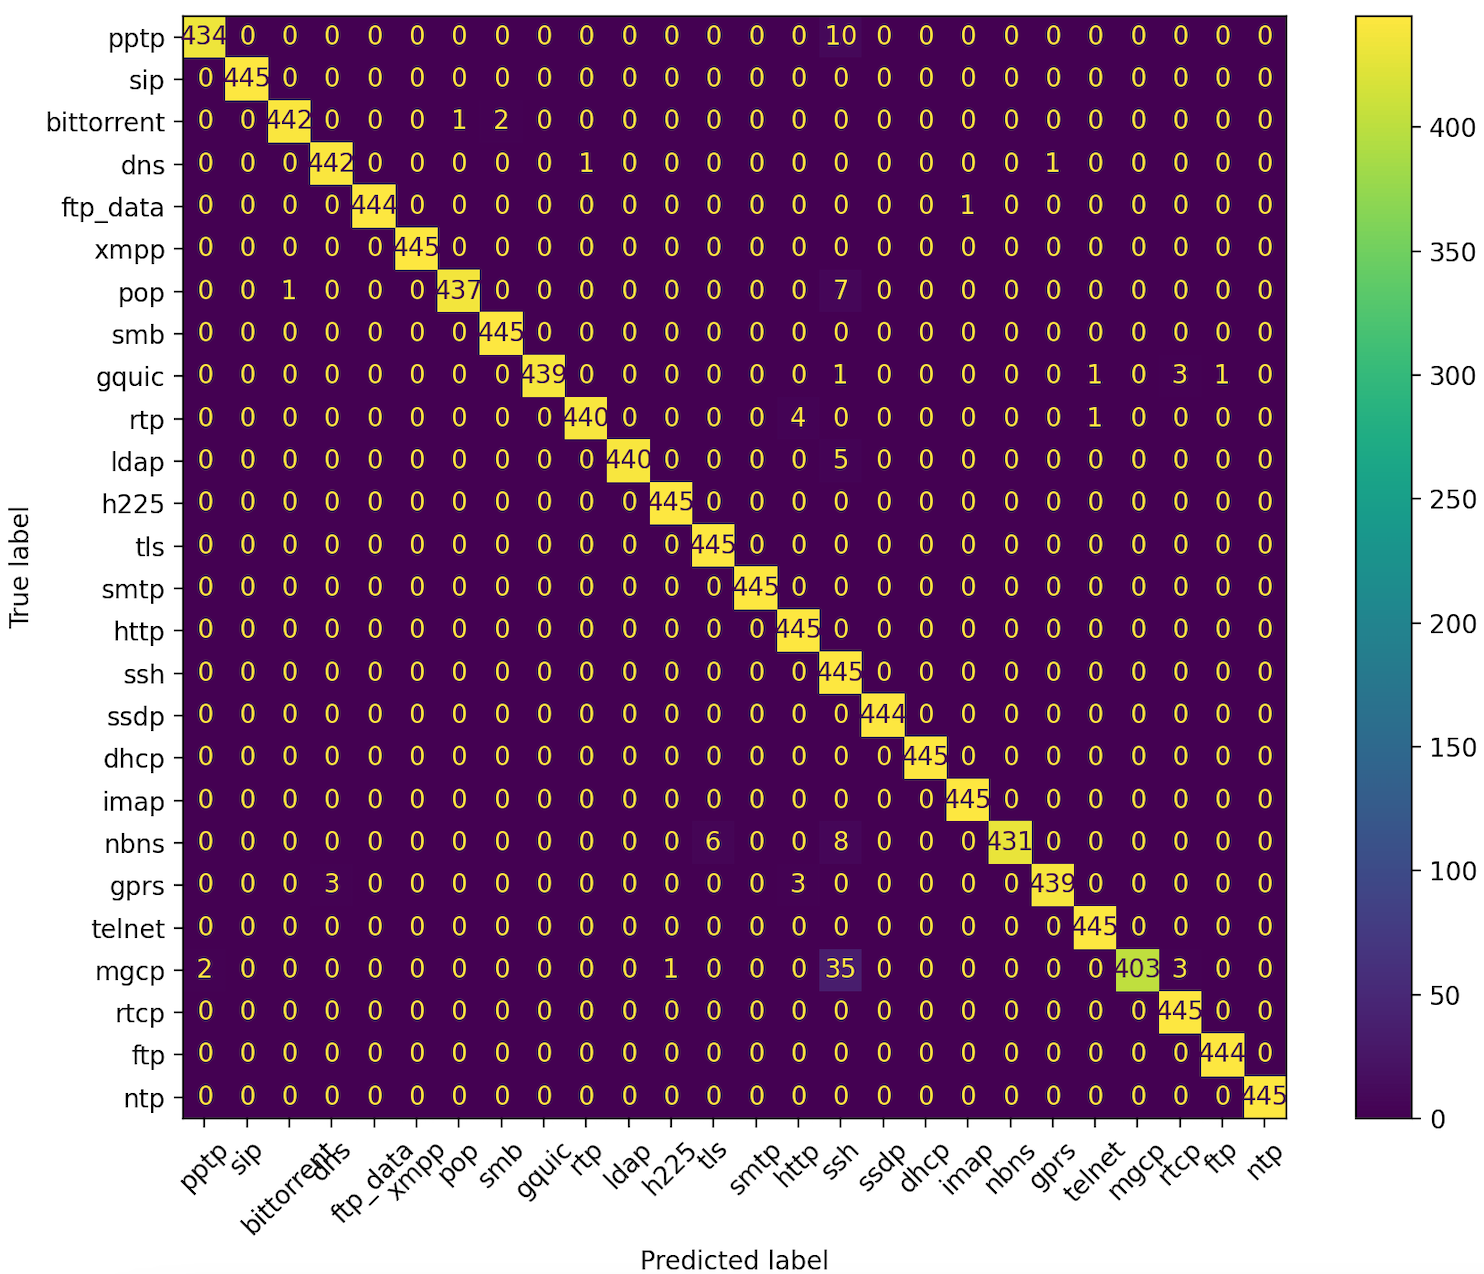
\includegraphics[width=\columnwidth]{chapters/4/img/combined.png}
  \caption{Twenty-six class identification problem using the \textsc{Alpine}-\textsc{Palm} combined model.}
  \label{fig:combined}
\end{figure}

\subsection{Traffic Type}

RFCs and standardized documentation necessitate that there are some detectable similarities between protocols. It is reasonable to think that detection of more abstract class types like traffic type (i.e. email, file transfer, web data) would be more heterogeneous and thus more difficult to embed. We experimented with classification by traffic type by amalgamating the dataset into classes as described in Table~\ref{table:dataset} in the datasets section of this work. Results in Figure~\ref{fig:trafficresults} show a confusion matrix of the classification results which are also highly accurate.

\begin{figure} [hbt!]
  \centering
  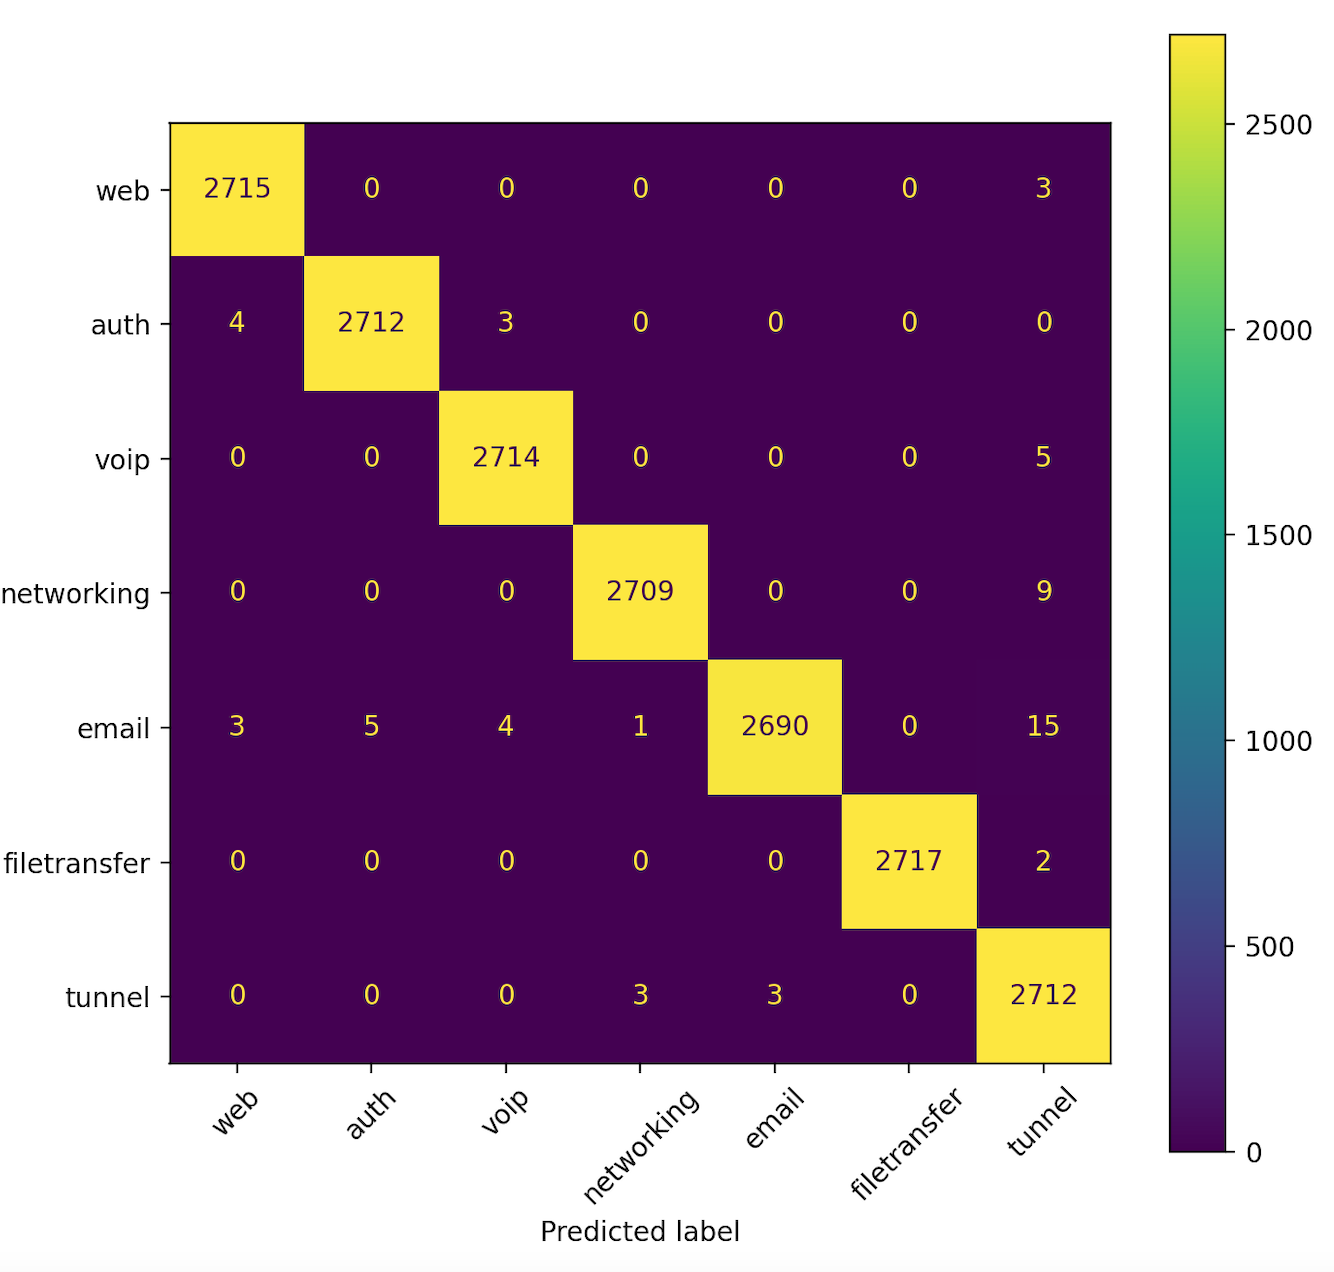
\includegraphics[width=0.8\columnwidth]{chapters/4/img/traffic_class_results.png}
  \caption{Confusion matrix of traffic type classification results.}
  \label{fig:trafficresults}
\end{figure}

\subsection{TF-IDF Score Evaluation}
In order to determine the effectivity of Jaccard similarity versus more complex similarity metrics, we evaluated the results of using payload tokens which were considered high-value by TF-IDF score. We posed this question to address concern that large data payloads, for example HTML documents or email messages, may introduce noise into hashes which would reduce classification accuracy. Instead, isolating payload tokens to only the high value ones could reduce spurious extra data. In order to test this, we implemented a TF-IDF measurement of tokens in the training stage. This was done by modifying configurations of the \textsc{Palm} model to filter the added tokens. When training and test signatures were generated, only those tokens with TF-IDF score above the minimum threshold were kept and included in the actual LSH signature. The results in Table~\ref{table:results1} show that this actually had a negative impact on the overall result, indicating the basic Jaccard similarity was a better distance metric for this use case.

\subsection{Multi-Embeddings}

\begin{table}
\caption{Multi-Hash Embedding Classification Results}
\centering
\begin{tabular}{| p{2cm} | p{0.6cm} p{0.6cm} p{0.6cm} || p{0.6cm} p{0.6cm} p{0.6cm} || p{0.6cm} p{0.6cm} p{0.6cm}|}
\hline
& \textbf{\textsc{Alpine}} & & & \textbf{\textsc{Palm}} & & & \textbf{Multi-Model} & & \\
\hline
\hline
\textbf{Accuracy} & 0.988 & & & 0.717 & & & 0.996 & & \\
\textbf{Cohen's~$\kappa$} & 0.988 & & & 0.705 & & & 0.997 & & \\
\hline
\hline
 \textbf{Protocol} & \textbf{F1} & \textbf{P} & \textbf{R} & \textbf{F1} & \textbf{P} & \textbf{R} & \textbf{F1} & \textbf{P} & \textbf{R} \\
 \hline
 BitTorrent & 0.98 & 0.97 & 1.00 & 0.74 & 0.75 & 0.73 & 0.99 & 1.00 & 0.99 \\
 DHCP & 1.00 & 1.00 & 1.00 & 0.91 & 0.83 & 1.00 & 1.00 & 1.00 & 1.00 \\
 DNS & 1.00 & 1.00 & 1.00 & 0.24 & 0.46 & 0.17 & 1.00 & 1.00 & 0.99 \\
 FTP & 0.96 & 0.97 &  0.94 & 0.90 & 0.83 & 0.98 & 0.99 & 0.99 & 1.00 \\
 FTPDATA & 1.00 & 1.00 & 1.00 & 0.20 & 0.37 & 0.13 & 1.00 & 1.00 & 1.00 \\
 GPRS & 1.00 & 1.00 & 1.00 & 0.91 & 0.98 & 0.85 & 1.00 & 1.00 & 1.00 \\
 GQUIC & 0.99 & 0.99 & 1.00 & 0.27 & 0.48 & 0.19 & 0.99 & 1.00 & 0.98 \\
 HTTP & 0.99 & 1.00 & 1.00 & 0.61 & 0.65 & 0.55 & 1.00 & 1.00 & 0.99 \\
 H.225 & 1.00 & 1.00 & 1.00 & 0.63 & 0.68 & 0.95 & 1.00 & 1.00 & 0.99 \\
 IMAP & 0.99 & 0.94 & 0.98 & 0.85 & 0.77 & 0.59 & 0.99 & 1.00 & 0.99 \\
 LDAP & 0.96 & 1.00 & 0.98 & 0.66 & 0.75 & 0.59 & 0.99 & 1.00 & 0.99 \\
 MGCP & 1.00 & 1.00 & 1.00 & 0.90 & 0.83 & 1.00 & 1.00 & 1.00 & 1.00 \\
 NBNS & 0.99 & 0.98 & 1.00 & 0.87 & 0.82 & 0.92 & 0.99 & 0.99 & 1.00 \\
 NTP & 1.00 & 1.00 & 1.00 & 0.90 & 0.82 & 0.99 & 1.00 & 1.00 & 1.00 \\
 POP & 0.99 & 0.98 & 0.99 & 0.26 & 0.41 & 0.20 & 0.99 & 0.98 & 1.00 \\
 PPTP & 0.99 & 0.98 & 0.99 & 0.49 & 0.33 & 1.00 & 0.98 & 0.95 & 1.00 \\
 RTCP & 1.00 & 1.00 & 1.00 & 0.92 & 0.85 & 1.00 & 1.00 & 1.00 & 1.00 \\
 RTP & 0.99 & 0.98 & 0.99 & 0.40 & 0.65 & 0.29 & 1.00 & 1.00 & 1.00 \\
 SIP & 1.00 & 1.00 & 1.00 & 0.93 & 0.87 & 1.00 & 1.00 & 1.00 & 1.00 \\
 SMB & 0.99 & 1.00 & 0.98 & 0.81 & 0.80 & 0.82 & 0.98 & 1.00 & 0.97 \\
 SMTP & 0.98 & 0.99 & 0.98 & 0.81 & 0.80 & 0.82 & 0.99 & 1.00 & 0.99 \\
 SSDP & 0.99 & 1.00 & 0.98 & 0.92 & 0.86 & 1.00 & 1.00 & 1.00 & 1.00 \\
 SSH & 0.95 & 0.97 & 0.92 & 0.47 & 0.67 & 0.37 & 0.99 & 1.00 & 0.98 \\
 Telnet & 0.99 & 0.98 & 1.00 & 0.80 & 0.75 & 0.85 & 0.99 & 0.99 & 1.00 \\
 TLS & 0.99 & 0.99 & 1.00 & 0.61 & 0.51 & 0.75 & 1.00 & 1.00 & 1.00 \\
 XMPP & 1.00 & 1.00 & 0.99 & 0.92 & 1.00 & 0.85 & 1.00 & 1.00 & 1.00 \\
 \hline
\end{tabular}
\label{table:embeddingresults}
\end{table}

The concatenation of multiple classifiers and agreeance among voters in an ensemble has yielded a reduction in error and at best correlation when there is a misclassification~\cite{tumerensemble}. We hypothesized that enabling both \textsc{Alpine} and \textsc{Palm} to run together would yield the most accurate and agreed-upon classification results. In order to test this, we ran the 26-class protocol identification test against configurations of the model with just \textsc{Alpine} embedding, only \textsc{Palm} embedding, and a final combined run. Our results as shown in Table~\ref{table:embeddingresults} demonstrate that the combined votes of both models turned out to be the most accurate in the final tests. Furthermore, the agreeance among voters was also highest using multiple hash embeddings.

\subsection{Model Performance and Throughput}
One critical requirement for applied machine learning in network processing is that systems must keep up with signal processing at very high rates. Any passive system must not interfere with legitimate traffic and service. Furthermore, the software must be capable of performing the necessary processing on as much of the traffic as possible (ideally, all of it). While thinning and load-balancing solutions as well as diverting and copying traffic for offline analysis can help levy this concern, there is still the desire to employ classification solutions at real-time rates. Thus, we perform experiments to see how the system scales based on model sizes and number of classes. We measured the training time, system throughput in millibits per second (Mbps) as well as memory usage during the testing phase in megibytes (MiB). We ran all performance tests on the combined dataset consisting of 140,157 total packets. In order to avoid bias we implemented random under-sampling to even out the distribution of data, causing our total number of packets after sampling to be a fraction from the original set. For testing the number of classes, we created experiments with binary RTP/non-RTP classification, the traffic-type multiclass experiment with 8 classes/types, and the largest 26-class experiment where we identify all possible data layer protocols. In Table~\ref{table:performanceresults}, we detail the results of the experiments for a varied number of classes and sample sizes.

\begin{table*} [ht!]
\caption{Performance Results for Varied Number of Classes}
\centering
\begin{tabular}{| p{0.11\linewidth} | p{0.1\linewidth} | p{0.1\linewidth} | p{0.1\linewidth} | p{0.1\linewidth} | p{0.1\linewidth} | p{0.15\linewidth} | p{0.1\linewidth} |}
\hline
Classes & \# Hashes & \# Samples & Training Time & Test Time & Memory Usage & Throughput & Accuracy \\
\hline
\hline
\textbf{RTP/ non-RTP} & 20,613 & 13,743 & 4.273s & 1.21ms & 470.8 MiB & 2.596 Mb\/s & 1.000 \\
\textit{Binary classification} & 2,400 & 1,600 & 0.738s & 0.866ms & 283.7 MiB & 3.139 Mb\/s & 0.997 \\
& 240 & 160 & 0.075s & 1.093ms & 353.4 MiB & 2.317 Mb\/s & 1.00 \\
\hline
\textbf{Traffic Type} & 28,543 & 19,029 & 7.136s & 1.015ms & 584.6 MiB & 3.728 Mb\/s & 0.997 \\
\textit{8-class problem} & 12,600 & 8,400 & 3.31s & 1.006ms & 305.3 MiB & 2.842 Mb\/s & 0.997 \\
& 240 & 160 & 0.683s & 2.397ms & 290.6 MiB & 2.54 Mb\/s & 0.998 \\
\hline
\textbf{Protocol} & 17,347 & 11,565 & 5.312s & 1.138ms & 352.4 MiB & 3.041 Mb\/s & 0.997 \\
\textit{26-class problem} & 15,600 & 10,400 & 3.13s & 0.727ms & 305.3 MiB & 4.231 Mb\/s & 0.998 \\
& 1,560 & 1,040 & 0.492s & 0.901ms & 301.8 MiB & 3.212 Mb\/s & 0.994 \\
\hline
\end{tabular}
\label{table:performanceresults}
\end{table*}

In order to test system scalability in deployment and verify the theoretical complexity discussed in the background section of this work, we performed a series of experiments increasing the number of signatures for a model used to classify HTTP traffic. As a comparator, we used the regular expression scanning tool built in RExACtor which uses the Hyperscan 5.4.0 regular expression matching library by Intel~\cite{hyperscan}. All experiments were performed on a single i9 Dell computer with Ubuntu 18.04 installed. In the trials, the number of signatures represented the number of LSH hashes our system or the number of regular expressions added to the sniffer application. We used RExACtor~\cite{rexactor} to generate HTTP signatures from the HTTP traffic in our dataset. Both models performed the classification with 100\% accuracy on all trials.

\begin{table}[ht!]
\centering
\begin{tabular}{| c | c | c | c | c |}
\hline
System & \# Signatures & Training & Testing & Memory \\
\hline
\hline
\textbf{\textsc{Alpine}/\textsc{Palm}} & 1,000 &  1.21s &  1.23s & 392.4 MiB \\
& 10,000 & 2.75s & 3.56s & 419.9 MiB \\
& 100,000 & 52.75s & 4.2s & 1047.4 MiB \\
& 1,000,000 & 423.3s & 4.52s & 4717.9 MiB \\
\hline
\textbf{Hyperscan} & 1,000 & 4.6s & 156ms & 70.7 MiB \\
& 10,000 & 81.8s & 1.3s & 529.3 MiB \\
& 100,000 & 39.9m & 17.28s & 4596.7 MiB \\
& 1,000,000 & 153m & 63.1s & - \\
\hline
\end{tabular}
\caption{Performance Results for \textsc{Alpine} and \textsc{Palm} as a multi-embedding versus Hyperscan}
\label{table:performanceresults}
\end{table}

\begin{figure} [ht!]
  \centering
  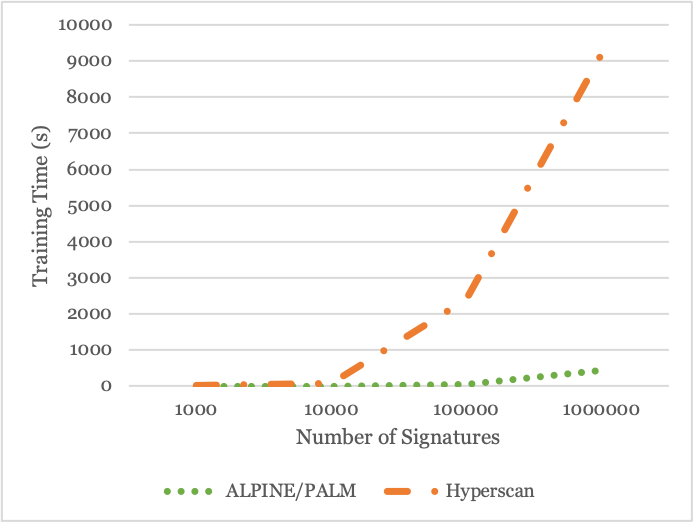
\includegraphics[width=0.6\columnwidth]{chapters/4/img/trainingtime.png}
  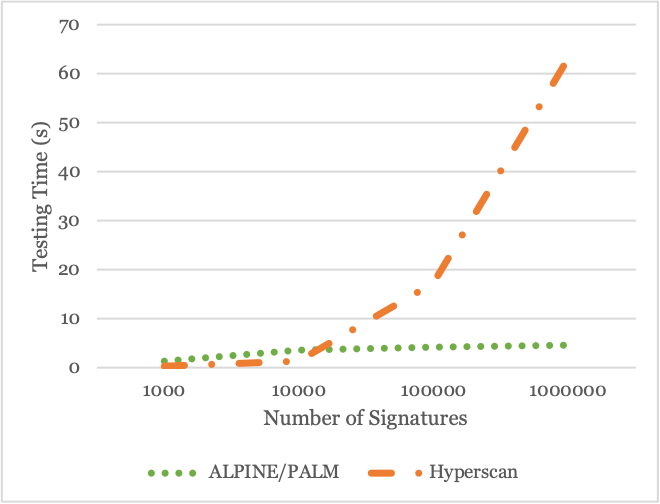
\includegraphics[width=0.6\columnwidth]{chapters/4/img/testingtime.png}
  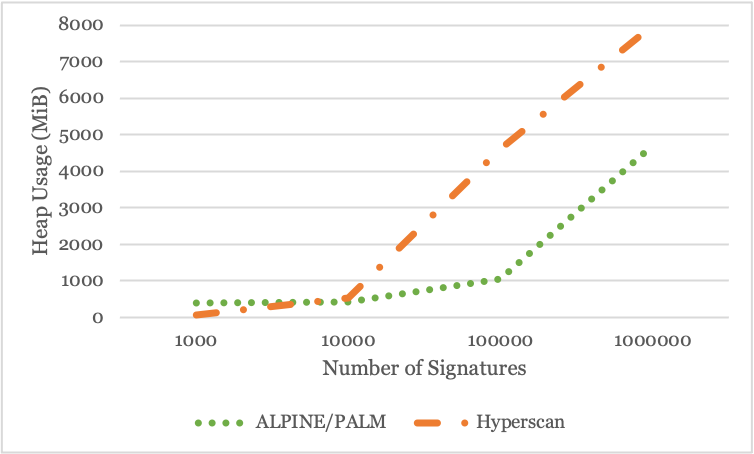
\includegraphics[width=0.6\columnwidth]{chapters/4/img/memoryusage.png}
  \caption{Time and space complexity results for \textsc{Alpine}/\textsc{Palm} versus Hyperscan.}
  \label{fig:hyperscancompare}
\end{figure}

\section{Discussion and Limitations}

The locality-sensitive hashing approach is an improvement upon the regular expression approach to DPI in several ways. First, the hash generation process reduces the need for expert knowledge about a particular protocol. Previously, engineers would have to employ unique signatures for different message types. It would not be uncommon, for example, to have regular expression signatures for every method for a given text-based protocol like FTP or IMAP. Furthermore, requests and response messages often require unique signatures. Regexes are difficult for humans to read and comprehend. The management of server-client side interactions is also a challenge to know which versions to apply. Instead, hash embeddings using our forward-thinking system create a unique value for each provided input and indexes those values into one bucket. This even more generally captures the broad diversity of possible payload and header contents while providing a new layer of abstraction and simplicity. Flows may be examined bi-directionally, and all message types and methods considered. We are also not limited to traffic flows and protocol types. As demonstrated by the experiments in this section, the system is capable of distinguishing more heterogenous or abstract class types like traffic type, mechanisms like encryption, and traditionally weak-signatured traffic like RTP. Furthermore, a single bad bit can cause a packet match on regular expression to fail. Network traffic and packets in the wild are extremely diverse and can be prone to error, and thus are an ideal test set for the multi-embedding hash technique which is both more informative and resilient. In terms of performance, the LSHForest as implemented in our model further reduces the storage and computational complexity when compared with a regular expression, automata-searching approach.

We posed the following research questions to assess the \textsc{Alpine} and \textsc{Palm} models and report our findings here:

\begin{itemize}
\item\textbf{R1.} Can packets be classified by application-layer potocol through the creation and index of locality-sensitive hashes?

Our model performed at a 99.6\% accuracy rate in its identification of many application layer protocols, indicating that locality sensitive hashes may be constructed which are highly representative of the data and low-cost for searching when indexed. This model may be expanded in real world implementations of DPI for traffic surveillance, cybersecurity and intrusion detection, quality of service managment and network management, content and copyright enforcement, and traffic profiling. Detecting the application layer protocol remains an important task for engineers. This hashing technique improves upon the available state of the art in both accuracy and breadth of scope in application.

\item\textbf{R2.} Does this model generalize to other kinds of network traffic classes besides protocol? Could we also distinguish more variable data such as email or VoIP traffic classes?

In addition to the application layer protocol, we also used traffic type labels on the dataset for experimentation. In this problem also the hash embedding technique proved highly accurate, which further demonstrates the generalizability of the models to new problems and real data.

\item\textbf{R3.} Does a different word embedding technique such as using only high-value tokens as characterized by TF-IDF score improve distance measure results? Will this reduce noise in the data and isolate important features?

We used Jaccard similarity as a baseline for comparison, but found that this distance metric was more effective than the TF-IDF score. This highlights a counterintuitive but significant point that challenges current network analysis trends. Machine learning techniques have become more technically advanced and often computationally intensive in order to improve model accuracy or other desired metrics. While TF-IDF decently diminishes tokens such as ``a'' and ``the'' from the English language, the fact that ``\textsc{HTTP\textbackslash1.1}'' appears in nearly every HTTP request in our dataset is actually relevant considering the context. Especially in network traffic analysis where scalability and line-rate capability is highly desirable, simple techniques can still be effective and should not be disregarded. Our experiments evidence that a more complex model is not always the appropriate direction. Even within subfields of machine learning like natural language processing, there is not a silver bullet solution which triumphs in every situtation. Rather, having multiple models to try or angles from which to consider the data seems to provide better, more well-rounded results.

\item\textbf{R4.} If we combined multiple hash embeddings, i.e. both \textsc{Alpine} and \textsc{Palm}, and concatenate their results, will there be an improvement in classification performance over a single hash embedding of the feature set?

Multi-embeddings are a proposed solution particularly for more heterogeneous datasets. This captures multiple angles or representations of the data and combines them for a more full-scope picture and analysis. In contrast, regular expressions provide only a one-dimensional viewpoint and are incapable of encoding highly variable data without impractical complexity and data over-selection. The modular design of our system enables using one or more embeddings, which allows for a balance between performance impact and accuracy. Interestingly, though the \textsc{Palm} model was overall poorer-performing than the \textsc{Alpine} model, votes from the \textsc{Palm} model helped improve the combined result regardless.

\item\textbf{R5.} Does the sample size, number of hashes, or number of classes significantly impact throughput or accuracy?

The performance impact of applied machine learning is a major concern for traffic analysis and cybersecurity. We provide transparent numbers of system performance to present the solution at scale. All experiments in this trial were run on a 1.6 GHz Dual-Core Intel Core i5 processor with 16GB DDR3 memory. In future work, leveraging an accelerated processor such as an FPGA would greatly enhance performance and throughput due to the repetitive nature of hash computations. The most impactful procedure based on system profiling is the MinHash step, which is likely optimizable through an FPGA~\cite{fpga}. The measure of acceptable throughput depends on the network environment; however, in terms of scalability it is valuable that our model is data independent in that it does not seem to increase exponentially or vary in performance wildly depending on the data. Our model also trains quickly, meaning that models could be swapped or trained online or in the field if needed. Future research could further optimize the process through batching and parallel processing. For example, it would be possible and beneficial to run training computations in parallel.Distance measures could also be taken in parallel for different models on separate threads and then the results aggregated.

\item\textbf{R6.} What is the rate of scalability of the system? Does it outperform state-of-the-art regular expression scanning in terms of testing/training time and memory usage?

We indicate in Table~\ref{table:performanceresults} that for small signature sets, Hyperscan initially outperformed our model; however, when scaled to larger signature sets, our model clearly is much more capable of handling the extra load. The comparative line graphs in Figure~\ref{fig:hyperscancompare} illustrate the exponential versus sublinear growth patterns of each measure of performance, clearly demonstrating our systems' scalability over the state of the art. In constructing models with 1 million signatures, our model takes just over 7 minutes while the Hyperscan implementation takes over 2 hours. At scale, even our testing time is much smaller than the baseline. Furthermore, at the 1 million signature scale our model uses just over 4GB of heap space, while Hyperscan crashed our setup due to exceeding 8GB of dynamic memory for 1 million signatures. This illustrates the point made earlier that no single model is best suited for every situation; rather, multiple models and strategies are needed for unique network environments. If the problem set or data structure size is small, Hyperscan could be an optimal choice; however, our model is more generalizable to larger data sets and adaptable to a variety of problems. It would not be unreasonable to scale to several million signatures in a real surveillance or DPI system which \textsc{Alpine} and \textsc{Palm} would be better suited for than the current capability of regular expression matching.
\end{itemize}

One key takeaway from the research done in \textsc{Alpine} and \textsc{Palm} is that multi-embeddings on packets in our given datasets and experiments were more effective at classifying the data than any single form of analysis. Naturally, this comes at the cost of generating more embeddings and thus increasing complexity and latency. Thus, when designing a multi-embedding model, there is a balance to be achieved between number of layers of representation and desired results. If storage space of models and embeddings or CPU utilization is of more concern than acute accuracy of classification, fewer or less complex representations may be required. The data may also be aptly divided for input into different models; for example, \textsc{Alpine} considers header features while \textsc{Palm} considers the payload.

\textsc{Alpine} and \textsc{Palm} show the potential for locality-sensitive measurements to consider multiple layers of features and are resilient to non-standard implementation. They normalize heterogeneous data into fixed-size, comparable space. These models as part of a DPI system have potential to scale both in performance and storage capacity. But, there are still problems in network classification that elude this method of feature extraction. For example, encrypted or compressed payloads make the text-based approach of \textsc{Palm} or regular expressions generated by \textsc{Rexactor} ineffective. Distinguishing encrypted traffic payloads from plaintext or compressed payloads is also a classification problem not appropriately dealt with through these methods. If \textsc{Alpine} features of the header are not enough alone to distinguish the traffic type or particular application the traffic represents, then the classification will be inaccurate. If the header is encrypted, this also renders \textsc{Alpine} ineffective. In further research, a method of understanding and profiling encrypted and compressed traffic or obfuscated payloads would greatly enhance deep learning-based DPI systems.


\chapter{MAPLE - IMAGE REPRESENTATION AND RECOGNITION OF INTERNET TRAFFIC}
\section{Introduction}

In chapters 3 and 4, we discuss the difficulty of generating token-based or regular expression-based signatures for weakly signatured, variable data. This type of data floods modern internet traffic today; examples would be voice-over-IP (VoIP), streaming services, downloads and file transfers, and peer-to-peer sharing. Furthermore, encrypted traffic payloads or compressed data make generating signatures from payload text ineffective. The tokenization strategy of \textsc{Palm} is defeated by these techniques, and as \textsc{Alpine} focuses only on header features there is still the problem of an unanalyzed payload with potentially useful, untapped information.

In 2021, it was projected that 3 billion people use VoIP technology as a regular part of their daily lives. In 2021-2022, Zoom reported over 300 million users~\cite{teamstage} Webex reported over 600 million, and Microsoft Teams recorded 275 million participants~\cite{businessofapps}. The widespread adaptation of VoIP technology has highlighted several cybersecurity vulnerabilities which make this type of traffic even more important to network intrusion detection systems. It is simple to spoof IP addresses or URIs with VoIP technology and produce robocalls used in phishing/spam or in denial of service attacks~\cite{edwards2020robocalling}. VoIP packet data is vulnerable to being the transport for backdoors, worms, trojans, and viruses which can be embedded~\cite{Wu2021SteganographyAS, nagaraja2019voiploc}. Cybersecurity specialists designing intrusion detection systems need to be able to intercept and process VoIP streams in order to detect these kinds of intrusions~\cite{choti2021prediction}. VoIP call analysis and reconstruction can also be used in the forensic environment to provide critical evidence of criminal activity. Policy or content rights violations or copyright infringement may also be detected through the analysis of the reconstructed calls~\cite{kmetfast, Sha2016VoIPFA}. This process and search capability is also useful to intelligence operations to find mission critical data from the enormous amount of traffic flowing in mission networks~\cite{kao2020forensic}.

A majority of mainstream VoIP protocols use the real-time transport protocol (RTP) as their transport layer for encapsulation. The application layer protocol, for example the Session Initiation Protocol (SIP), Media Gateway Control Protocol (MGCP), or H.248, will establish the connection between endpoints and carry important session information such as codec encoding and metadata for the call. The application then relies on RTP to manage the dataflow between the connected systems. In the \textit{complex, real network environment}, the implementation of SIP and RTP data flow is often sent de-coupled across physical signals and ports which presents a challenge for cybersecurity specialists using middlebox technologies for packet inspection and call reconstruction. Because the RTP data is encoded, it is necessary to know the signaling information in order to retrieve the codec information for proper decoding. Furthermore, the metadata associated with signaling protocols such as the SIP URI identifier provides necessary enrichment and context for the actual call. Lastly, RTP data may arrive at the middlebox before the signaling information which contains the port numbers associated with the RTP stream for that particular call; thus, the middlebox must retrospectively identify data packets (RTP) which belong to particular signaling information headers (SIP, for example).

Detecting the RTP stream itself from other types of traffic can be a difficult problem because the RTP signature is weak and can be further obfuscated by encryption (SRTP). The problem of accurately classifying network traffic has expanded beyond the scope of capability of text-based solutions. Instead, we propose using higher dimensionality of network traffic in order to advance RTP detection capability. \textsc{Maple} is a \underline{\textbf{ma}}trix-based \underline{\textbf{p}}ay\underline{\textbf{l}}oad \underline{\textbf{e}}ncoder which transforms packets into grayscale images to unveil hidden representation which may be used as input into a convolutional neural network model. Using this approach, we are able to expand detection capability to weakly signatured data, encrypted versus compressed traffic, and better traffic type and application profiling.

\section{Previous Work}

Data in convolutional neural networks are organized into three aspects which determine the spatial dimensionality of the input: the height, width, and depth. The data engineering design processes pixelated data and discovers visual patterns in the latent space.

Following the input layer, there are three layer types which make up the CNN model. A \textit{pooling} layer performs down-sampling along the spatial dimensionality of the given input in order to reduce dimensions. For each feature map $a^l_{i, j, k}$, pooling can be calculated as follows:
\begin{equation}
    y^l_{i, j, k} = pool(a^l_{m, n, k}), \forall(m, n) \in R_{ij}
\end{equation}

where $R_{ij}$ represents the local neighborhood around point $(i,j)$. Common pooling functions include max pooling and average pooling~\cite{gu2018recent}. A \textit{convolutional layer} uses a kernel filter in order to compute feature maps. The feature value of location $(i, j)$ in the $k$th feature map of the $i$th layer $z^l_{i, j, k'}$ is calculated by:
\begin{equation}
    z^l_{i, j, k} = w^{l^{T}}_kx^l_{i, j} + b^l_k
\end{equation}

where $w_k^l$ and $b_k^l$ are the weight vector and bias term of the $k$th filter at the $l$th layer. The activation function, usually sigmoid, tanh, or rectified lineur unit (ReLU), may then be calculated as:
\begin{equation}
    a^l_{i, j, k} = a(z^l_{i, j, k})
\end{equation}

 Finally, \textit{fully-connected} layer takes input from the previous layer and connects them to neurons of the output layer in order to perform high-level reasoning or learn some global semantic information~\cite{OShea2015AnIT}.

LeNet~\cite{lenet} consists of two sets of convolutional, activation, and pooling layers. There is also a final set of consisting of fully-connected, activation, and fully-connected layers which proceed to a softmax normalization and classification at the output layer.

Deep neural networks suffer from accuracy degradation due to how difficult it can become to map intermediary or residual layer outputs to inputs. Thus, a residual convolutional neural network (ResNet) is built up of blocks of stacked layers formed from a series of convolutions and non-linear activation functions. Following the authors who first introduced deep residual networks~\cite{resnet}, we define a block as:
\begin{equation}
    y = F(x, \{W_i\}) + x
\end{equation}

Where $x$ and $y$ are the input and output vectors, respectively, and $F(x, \{W_i\})$ is the residual mapping with a set of weights $W_i$. If $H(x)$ represents the ideal output mapping that corresponds to the ground truth, residual networks hypothesize that $F(x) + x = H(x)$. The residual function is pushed to zero such that the equation becomes an identity function $H(x) = x$. This identity mapping, or shortcut layer, is what reduces the degradation problem and minimizes training error as the network becomes deeper~\cite{resnet}.


In previous work, CNNs have been employed to classify network traffic both for per-packet and per-flow scenarios. Lim et al~\cite{lim2019network} also transform packets into grayscale images and use CNN and ResNet architectures to label them by application (RDP, Skype, BitTorrent, and others). When using payloads of 1024B and a ResNet architecture, they achieved a 0.97 F1 score for accurately classifying the packets as one of eight types of applications.

Yang et al~\cite{yang2022} transform network packets in creative adversarial networks (CANs) using quantile normalization which generate pixelated images for CNN processing. They combine multiple packets into a single image for flow-based processing. For example, they propose taking 27 packets with 9 features each and creating a $9 \times 9 \times 3$ image, where three channels RGB (red, green, blue) are provided for a single pixel. This is then used as input into their CNN architecture.

Gao~\cite{Gao2022} proposed a CNN-LSTM architecture which reduces false positive rates in their network intrusion detection system for cloud computing environments. Numerical and character attributes from the KDD CUP 99 test data set are first pre-processed into a $10 \times 42$ matrix, where window size $w = 10$ and the number of features in the data set is 42. The data set is transposed to an image dataset where each matrix $W$ is mapped to a $10 \times 42$ grayscale image. If $v_{ij}$ represents the value of a pixel in matrix/image $W$ at position $i,j$, the values $v_{ij} \in [0,255]$. To reduce the data interval and normalize values, the following formula is used:
\begin{equation}
    x = \frac{x-\overline{x}}{\delta}
\end{equation}

where $x$ is the current value of a certain data in the sequence, $\overline{x}$ is the mean value of the data in the series, and $\delta$ is the standard deviation of the sequence. Finally, this system adds an additional attention mechanism layer to improve classification accuracy:
\begin{equation}
    \begin{split}
    u_t = tanh(W_wP_t + b_w), \\
    a_t softmax(u_t^T, u_w), \\
    v = \sum a_tP-T,
    \end{split}
\end{equation}

where $u_t$ is the attribute representation of $P_t$, $W_w$ is the context vector randomly generated during training, $a_t$ is the importance weight, and $v$ is the high-level representation obtained through importance weight summation on $P_t$. \\

Jo et al~\cite{jo2020packet} use a CNN-LSTM hybrid model to perform network intrusion detection, but first pre-process packets into image representations. Namely, they adapt the NSL-KDD dataset which has 41 fields into pixel representations. Continuous fields are first normalized to a $[0-255]$ range to create a grayscale image pixel value. Symbolic fields such as ``protocol type'' are represented by the same kind of pixel value, but normalized based on the number of possibilities. For example, a symbolic value with three possibilities will be normalized as 0, 128, or 255~\cite{jo2020packet}. $28 \times 28$ images are created and processed with a $5 \times 5$ kernel as shown in Figure~\ref{fig:kernel}.

\begin{figure} [h!]
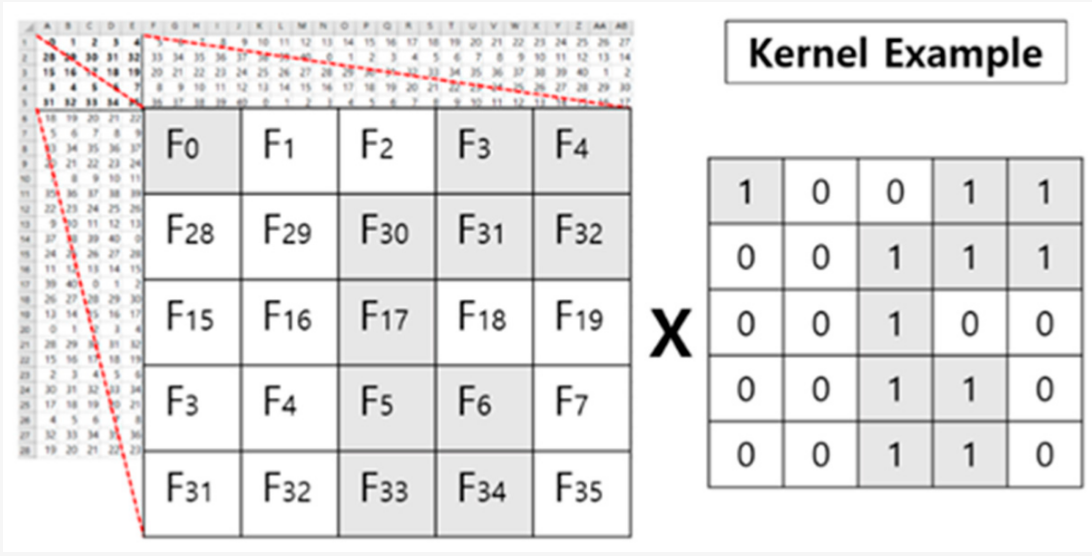
\includegraphics[width=\linewidth]{chapters/5/img/kernel.png}
\caption{Example application of kernel to pixelated packet data~\cite{jo2020packet}}
\label{fig:kernel}
\end{figure}

Deep Packet~\cite{deeppacket} is a well-cited work in deep learning for traffic classification. In this system, a stacked auto-encoder and CNN are employed to classify traffic by type and application as labeled in the VPN/non-VPN UNB ISCX dataset~\cite{vpn-dataset}. Their solution achieves 94\% accuracy in the traffic classification task per traffic type, and 97\% accuracy in the application classification task. Incorporating the same dataset as well as additional, more recent flows, we are able to achieve higher accuracy in RTP detection with a less computationally complex framework in \textsc{Maple}.

\section{Methodology}

We expect some level of standardization (i.e. method names or status codes) or some commonalities such as user names, device details, semantic contexts, and other conversation or implementation-specific indicators even in highly entropic or variable packet data. Using this hypothesis, \textsc{Maple} transforms packets into grayscale images which will appear similar to one another. Thus, machine learning algorithms designed for image analysis may record the hidden features generated from the similarities between the two images. We base this assumption on previous work~\cite{lim2019network} which has shown similarities in grayscale images rendered from packet data in order to classify traffic by application and protocol type which are detectable by CNNs. Figure~\ref{fig:grayscale} asserts the validity of this assumption by showing comparative images rendered from packets in our combined dataset previously used and explained in detail in chapter 4 of this work.

\begin{figure} [ht!]
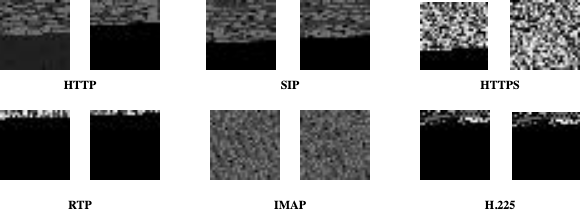
\includegraphics[width=\linewidth]{chapters/5/img/grayscaleimages.drawio.png}
\caption{Grayscale images generated from packets in our combined dataset used in the following experiments.}
\label{fig:grayscale}
\end{figure}

To shape packet payloads into an image, we extract the payloads and convert them from byte encoding to a normalized decimal integer $i \in [0,255]$~\cite{jo2020packet}. For image size, we chose a $28\times28$ representation, for a total of 784 input features. Padding is applied in the cases where the payload is shorter than 784 bytes, and is otherwise truncated.

\subsection{LeNet Model Configuration}

\begin{figure} [ht!]
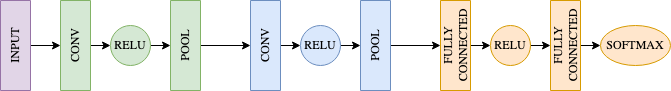
\includegraphics[width=\linewidth]{chapters/5/img/lenet.drawio.png}
\caption{The architecture of our LeNet models.}
\label{fig:lenet}
\end{figure}

LeNet was one of the standard models we selected in order to test convolutional neural networks against the RTP detection problem. LeNet has a low complexity, so has higher potential for practical use in real-time, line-rate packet inspection systems than deeper models which require more time. Figure~\ref{fig:lenet} shows the set up of the model which we use as a baseline. We designed two separate models where one employed $6$ and $16$ kernels per convolutional layer (A) and another that used a $16$ and $32$ kernels (B). Each model contained two fully-connected, dense layers of size $1024$ with a binary softmax classifier at the output layer.

\subsection{ResNet Model Configuration}

\begin{figure} [ht!]
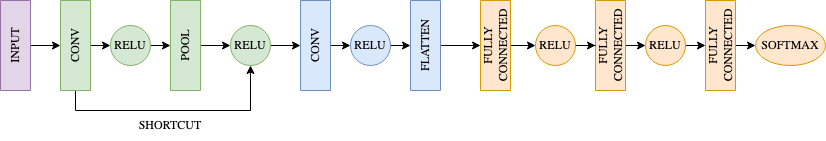
\includegraphics[width=\linewidth]{chapters/5/img/resnet.drawio.png}
\caption{The architecture of our ResNet models.}
\label{fig:resnet}
\end{figure}

If they are to be deployed at scale, artificial intelligence solutions must be capable of line-rate processing while still being able to perform the classification task to the required level of accuracy. This can be difficult to quantify as the definition of line-rate varies per network environment. Still, we assert that the identity mappings of ResNet do not introduce additional complexity~\cite{resnet}. Thus, residual mapping is introduced as a potential solution to adding additional layers of representation and thus improve classification through more hidden features, while also minimizing overhead.

We developed four ResNet-based models for the \textsc{Maple} system's experiments. The first model (C) consists of three convolutional layers with $32$, $32$, and $64$ kernels of dimension $3\times3$, and three dense layers with output sizes of $64$, $32$, and $2$ respectively. The second model (D) follows a similar architecture except the values are halved. Convolutional layers had $16$, $16$, and $32$ kernels per layer and the three dense layers had output sizes of $32$, $16$, and $2$. Model (E) corresponds to the same number of kernels and output sizes as (C), except it uses a kernel dimension of $7\times7$. The ReLU activation function and adam optimizer was used in all the model configurations, and a final layer used softmax for normalization and classification. The loss function used for training was categorical cross-entropy, and we also employed a dropout layer to reduce overfitting.

\begin{table} [h!]
\centering
\begin{tabular}{| l | l | l | l | l |}
\hline
Type & Model & \# Kernels & Kernel Size & FC Dim \\
\hline
LeNet & A & $3\times3$ & 6, 16 & 1024, 2 \\
\cline{2-5}
& B & $3\times3$ & 16, 32 & 1024, 2 \\
\hline
ResNet & C & $3\times3$ & 32, 32, 64 & 64, 32, 2 \\
\cline{2-5}
& D & $3\times3$ & 16, 16, 32 & 32, 16, 2 \\
\cline{2-5}
& E & $7\times7$ & 32, 32, 64 & 64, 32, 2 \\
\cline{2-5}
\hline
\end{tabular}
\caption{Configurations of each model used in the experiments.}
\label{table:attacks}
\end{table}

\section{Experiments and Results}

We ran several experiments to test the model's ability for binary RTP/non-RTP detection as well as multi-class protocol identification. All tests were performed on a single CPU of a 1.6 GHz dual-core Intel i5 processor with 16 GB DDR3 RAM. In the binary confusion matrix, true positive (TP) indicates correct classification of data. True negative (TN) is correct classification of data as non-RTP. false negative (FN) implies incorrect identification of traffic as non-RTP, and false positive (FP) is the incorrect classification of data as RTP. We use measurements of precision, recall, and F1-score for model evaluation, defined as follows:

\begin{equation}
\begin{split}
    Recall = \frac{TP}{TP + FP} \text{  }
    Precision = \frac{TP}{TP + FN} \\
    F1\text{ }Score = \frac{2(P\times R)}{P + R} \\
    \end{split}
\end{equation}

\subsection{RTP Detection}

For the binary RTP/non-RTP classification, we re-labeled all non-RTP and non-SRTP traffic as \textit{non-RTP}, and merged SRTP and RTP traffic into an \textit{RTP} label. For testing the different configurations of the \textsc{Maple} model, traffic was first processed and transformed into a matrix image, and then used as input for each of the models. We performed random under-sampling to avoid bias in the dataset, and then split the data into 60\%/40\% for training and testing. First, in order to establish a baseline we ran the multi-model using \textsc{Alpine} and \textsc{Palm} with the same datasets with the results in Table~\ref{tab:rtpresultslsh}. We ran tests with training for $3$ epochs for each CNN model. As we plan to deploy this technology in a real RTP detection and deep packet inspection system, we also measured classification throughput in order to determine how much traffic the \textsc{Maple} system would be able to process given the detection model configuration. Results are provided in Table~\ref{tab:binaryresults}.

\begin{table} [h!]
\centering
\begin{tabular}{| r | c | c | c |}
\hline
Class & P & R & F1 \\
\hline
\textit{Non-RTP} & 0.73 & 0.77 & 0.75 \\
\textit{RTP} & 0.76 & 0.71 & 0.73 \\
\hline
\end{tabular}
\caption{Classification results of RTP vs non-RTP detection for the LSH model.}
\label{tab:rtpresultslsh}
\end{table}

\begin{table} [h!]
\centering
\small
\begin{tabular}{| r | c | c | c |}
\hline
Model & P & R & F1 \\
\hline
\textbf{A} &&& \\
\textit{Non-RTP} & 0.96 & 0.99 & 0.98 \\
\textit{RTP} & 0.99 & 0.96 & 0.98 \\
\hline
\textbf{B} &&& \\
\textit{Non-RTP} & 0.97 & 0.99 & 0.98 \\
\textit{RTP} & 0.99 & 0.97 & 0.98 \\
\hline
\textbf{C} &&& \\
\textit{Non-RTP} & 1.00 & 0.99 & 1.00 \\
\textit{RTP} & 0.99 & 1.00 & 1.00 \\
\hline
\textbf{D} &&& \\
\textit{Non-RTP} & 1.00 & 1.00 & 1.00 \\
\textit{RTP} & 1.00 & 1.00 & 1.00 \\
\hline
\textbf{E} &&& \\
\textit{Non-RTP} & 1.00 & 1.00 & 1.00 \\
\textit{RTP} & 1.00 & 1.00 & 1.00 \\
\hline
\end{tabular}
\caption{Classification results of RTP vs non-RTP detection for all \textsc{Maple} models.}
\label{tab:binaryresults}
\end{table}

\begin{table}
\centering
\small
\begin{tabular}{| r | c | c |}
\hline
Model & Accuracy & Mb/s \\
\hline
\textbf{A} & 0.975348 & 12.5 \\
\hline
\textbf{B} & 0.978258 & 9.28 \\
\hline
\textbf{C} & 0.996934 & 7.07 \\
\hline
\textbf{D} & 0.995908 & 10.41 \\
\hline
\textbf{E} & 0.996847 & 5.3 \\
\hline
\end{tabular}
\caption{Throughput results of RTP vs non-RTP detection for all \textsc{Maple} models.}
\label{tab:binarythroughput}
\end{table}

Generally, the ResNet model performed exceedingly well at the RTP detection task, exceeding ninety-nine percent accuracy across all the configurations. The LeNet models performed marginally worse in terms of accuracy, but the smaller of the two models had the highest throughput of any of the tested configurations. Another configuration choice which may have significant impact on model accuracy is the number of epochs trained. Real systems place an emphasis on minimizing down time of a system, but in actual deployment many models may be trained offline and then embedded. In systems where training time is not a factor of performance, we can thus increase the number of epochs with little real impact. In order to test the efficacy of such a design choice, we re-ran \textsc{Maple} models A and C with 10 epochs to see if performance improved. Results in Tables~\ref{tab:addepoch1} and ~\ref{tab:addepoch2} show that ResNet appears to learn faster than LeNet, as it gained very little improvement with additional training time. Interestingly, with additional training time LeNet approaches similar accuracy to ResNet but still maintains higher throughput.

\begin{table} [h!]
\centering
\small
\begin{tabular}{| r | c | c | c |}
\hline
Model & P & R & F1 \\
\hline
\textbf{A} &&& \\
\textit{Non-RTP} & 0.99 & 0.99 & 0.99 \\
\textit{RTP} & 0.99 & 0.99 & 0.99 \\
\hline
\textbf{C} &&& \\
\textit{Non-RTP} & 1.00 & 1.00 & 1.00 \\
\textit{RTP} & 1.00 & 1.00 & 1.00 \\
\hline
\end{tabular}
\caption{Classification results of RTP vs non-RTP detection for \textsc{Maple} models A and C with additional training time.}
\label{tab:addepoch1}
\end{table}

\begin{table} [h!]
\centering
\small
\begin{tabular}{| r | c | c |}
\hline
Model & Accuracy & Mb/s \\
\hline
\textbf{A} & 0.990499 & 14.99 \\
\hline
\textbf{C} & 0.998172 & 7.38 \\
\hline
\end{tabular}
\caption{Throughput results of RTP vs non-RTP detection for \textsc{Maple} models A and C with additional training time.}
\label{tab:addepoch2}
\end{table}

\subsection{Protocol Auto Detection}

As previously mentioned, many middlebox technologies are interested in multi-classification problems where many different applications or protocols need to be identified. Thus, we expand our experiments to a 26-protocol problem using the combined dataset described in chapter 4. We again use models A and C, LeNet and ResNet respectively, for this expansion. As this is a much harder problem, we expect to need more training time. We ran each model with 10 epochs and 50 epochs, and recorded the macro averages in Table~\ref{tab:multiresults}.

\begin{table} [h!]
\centering
\begin{tabular}{| r | c | c | c | c |}
\hline
Model & P & R & F1 & Accuracy \\
\hline
\textbf{A - 10 epochs} & 0.78 & 0.78 & 0.77 & 0.780920\\
\textbf{50 epochs} & 0.83 & 0.83 & 0.83 & 0.832446 \\
\hline
\textbf{C - 10 epochs} & 0.84 & 0.84 & 0.83 & 0.835993 \\
\textbf{50 epochs} & 0.86 & 0.85 & 0.85 & 0.849528\\
\hline
\end{tabular}
\caption{Results of multi-class detection for models A and C as macro averages.}
\label{tab:multiresults}
\end{table}

Increasing the training time for the LeNet model showed significant improvement in accuracy, but not likely to a level needed for deployed systems so there is a need to build upon the baseline. The ResNet model approaches better accuracy with more training time.

\subsection{Model Performance and Throughput}
Decreasing the number of kernels may have slightly impacted accuracy, but improved overall throughput significantly and lessens memory footprint. In a real network environment, it may be worth consideration to sacrifice some accuracy in order to be able to monitor more traffic or more effectively load-balance the received input depending on hardware capability. Thus, the ideal model configuration is often environment-dependent and inspired us to incorporate configuration capability in \textsc{Maple} so that the deployed system may best suit the environment. We provide the throughput of each model configuration in our experiments in Table~\ref{tab:binarythroughput}.

\section{Discussion and Limitations}
\textsc{Maple} works well on input data such as a payload which may be distinct from one data sample from another, but can be divided and matricized into units for comparison (i.e. turned into a grayscale image of uniform dimension). For deep packet inspection, this model is able to create latent representations of payload data which uniquely identify traffic of different types at a higher dimension than is considered by current signature-matching or filter-based solutions used in industry. Our implementation for this initial deployment solves the RTP detection problem with high accuracy using a minimal framework ideal for line-rate. The system could be further optimized by running these models in parallel; as the solution relies on per-packet analysis, throughput could be increased across models. One limitation of the proposed encoding is that individual packets must be large enough to create a significant image. Thus, this model would not work well on short packets or packets with no payload data. In this case, we propose using a combination of header features and payload when available would be a wiser strategy.


\chapter{DATE - POINT CLOUD REPRESENTATION AND DENSITY CLUSTERING ANALYSIS OF PACKETS}
\section{Introduction}

While image generation and matrix representation expand packet data to two-dimensional space, we wanted to explore other geometric representations of data and deepen the dimensionality. In geometric topology, point clouds are another way to generate data shapes for anomaly detection and comparison. We propose ~\textsc{Date}, a cluster \underline{\textbf{d}}ensity \underline{\textbf{a}}nalysis-based \underline{\textbf{t}}ensor \underline{\textbf{e}}ncoder model which expands network packets into three dimensional point clouds, which we then extract features of regarding cluster density in order to find commonalities and classify based on data shape. This spatial expansion is a novel application of latent representation learning to network traffic and the problem of RTP detection or detecting weakly signatured traffic and could expand to other protocol problems.

\section{Previous Work}

\textsc{DATE} is a novel contribution to the field of packet processing as there is little published, previous work in generating 3D point cloud representations of packets. Raw packet data from LiDAR (light detection and radiation) systems have been shaped losslessly into 2D matrices and point clouds~\cite{Tu2019point}. This work introduces the problem of spatial correlation in packet data, namely that packets in their raw state are not usually uniform or in a state which may be processed using the spatial or geometric strategies employed by image and computer vision algorithms. Thus, data compression or pre-processing must be performed to create the necessary uniformity.

Costeux et al~\cite{costeux2006detection} worked on the fast detection of Skype and other RTP-based telephony traffic. They specify several fields from the RTP and encapsulation header which can be used to filter out non-RTP traffic. We employ this technique in the middlebox as an initial filtering step in our end-to-end data processing pipeline.

Kmet et al~\cite{kmetfast} build on Costeux by incorporating additional header features for per-packet selection, and adding a flow-based solution to reduce the over-selection problem. They were able to minimize mis-classification to nearly zero by buffering up to 10 packets of the RTP stream. The synchronization source number from the header is used along with timestamps to check for proper increment and stream correlation. We focus on per-packet identification only.

Some early research~\cite{patwari2005manifold} describes expanding NetFlow data generated by routers into 2D manifolds. We reference this as an intial introduction of spatial expansion of traffic data in order to perform dimensionality reduction, which is a key theoretical linkage to our work.

\section{Methodology}

\textsc{Date} describes the density-based clustering analysis which is a novel contribution of this work. This process attempts to map data to a three-dimensional space, then use spatial features to generate hidden features.

\subsection{Point Cloud Creation}
Point clouds are a set of Cartesian coordinates $(x, y, z)$ which represent some points in a three-dimensional space. Point clouds may be used in computer vision software as a method for mapping high-dimensional shapes into lower-dimensional space~\cite{Wang_2019_ICCV}. As a latent representation, this method can be used temporally to express the movement of objects in three-dimensional space. An airplane can be modeled as a three-dimensional point cloud, and its movement described as a series of clouds ${c_0, c_1,...,c_t}$ where $t$ represents a number of time intervals and $c_n$ the point cloud generated at a given time slice. Like the work of Quach et al~\cite{Quach2020compression}, we do not combine multiple representations in a time series but instead analyze the static representations much analagous to manifolds in three-dimensional space. We use the geometrical representation captured here for cluster analysis.

\begin{figure} [ht!]
\centering
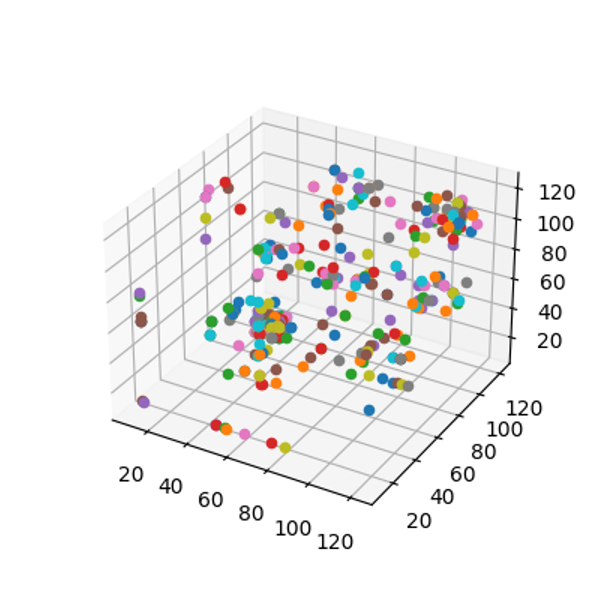
\includegraphics[width=0.6\textwidth]{chapters/6/img/sipcloud.png}
\caption{3D point cloud made out of a Session Initiation Protocol (SIP) packet}
\label{fig:cloud}
\end{figure}

In the \textsc{Date} model, payload data is extracted from the packets and truncated to 1024 bytes. If the payload is shorter than this, we add padding for normalization. Byte values $v$ are converted to decimal values $v' \in [0,255]$. For example, the byte string, `0x68', `0x65', `0x6c', `0x6c', `0x6f', would first be transformed to decimal values (104, 101, 108, 108, 111). Then, the sliding window would produce the points corresponding to coordinates:
\begin{equation}
\begin{split}
     C =
\{(104, 101, 108), \\ (101, 108, 108), \\ (108, 108, 111)\}.
\end{split}
\end{equation}

The coordinates are mapped to a three-dimensional space to form point clouds like Figure~\ref{fig:cloud}. We expect that similar point clouds will be generated from packets with similar data.


\subsection{Density-Based Spatial Clustering of Applications With Noise (DBSCAN)}

Density-Based Spatial Clustering of Applications with Noise (DBSCAN) uses three different point classifications. \textit{Core points} make up the centers of clusters. Individual core points are labeled based on the number of neighbors they have compared to their neighbors, or their degree of importance. \textit{Border points} are those which have the least number of neighbors but are still comparatively relevant due to being within the range of a core point. These comprise the edges of the point cloud. \textit{Outlier points} are neither borders nor cores, do not belong to a cluster, and are considered noise~\cite{schubert2017dbscan}. The DBSCAN algorithm visits each point and classifies them as such in order to paint a picture of where clusters of data are as in Figure~\ref{fig:dbscan}.

\begin{figure} [ht!]
\centering
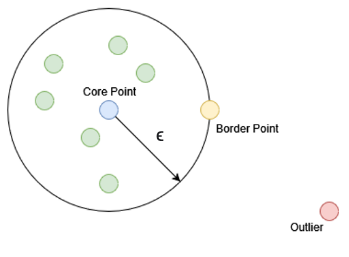
\includegraphics[scale=0.4]{chapters/6/img/dbscan.drawio.png}
\caption{Illustration of types of points in DBSCAN}
\label{fig:dbscan}
\end{figure}

We first create the point clouds and then process them using DBSCAN in order to derive the natural clusters that exist in the data. DBSCAN groups points that are close together utilizing a Euclidean distance for measurements. The value of the Euclidean distance that determines proximity and the minimum number of points needed to form a cluster are configurable parameters: $\epsilon$ and a minimum number of samples. The $\epsilon$ value is the radius for each circle drawn around each point to query density, and the minimum number of samples is the minimum number of points required to be inside the drawn circle for it to be considered a Core point.

Generally, the number of samples is twice the dimensions, but it must be at least the number of dimensions. If it is set below this threshold, then singular points or two points that are close together would constitute a cluster, which would not be an accurate way of determining where data is clumped~\cite{mullin2020tuning}. In our experiments, we configured DBSCAN to perform with $\epsilon$ = 7 and \texttt{min\_samples} = 7. This would be enough to create more clusters in a less populated point cloud. An $\epsilon$ value of 7 also allowed for a greater number of recognizable clusters~\cite{rahmah2016determination}.

Like many machine learning models, the parameters used to tune DBSCAN greatly affect performance rates. It is possible to create more clearly defined point clouds within the three-dimensional space through this parameter adjustments. The $\epsilon$ value needs to be set based on general rules. If the value of $\epsilon$ chosen is too small then too many clusters will be created which over-emphasize the importance of noisy points. However, if set too large, then clusters will merge together and shapes become less distinct. One way that a value of $\epsilon$ can be estimated is by examining the input data and finding the average distance between each point and its $K$-nearest neighbors. Choosing an exact value for $\epsilon$ is a difficult problem for packet data which is highly variable. The $\epsilon$ value must be estimated from a conglomeration of the packet's $K$-nearest neighbors where $K$ is equal to \texttt{min\_samples}.

Because each packet is highly variable, choosing an exact value for $\epsilon$ is a difficult problem. An estimation of $\epsilon$ must be taken from a conglomeration of the packet's $k$-nearest neighbors data where $k$ is the value of \texttt{min\_samples} chosen. As shown in the figure above, the point of each line with the greatest curvature is considered the ideal value for $\epsilon$. A line has been illustrated in Figure~\ref{fig:kneighborsgraph} where an estimated average is made for every sample. The variation in an ideal $\epsilon$ value could be a major factor in why some packets are recognizable in their cloud state and others are not~\cite{rahmah2016determination}.

We extract the following features as the feature vector for classification from the DBSCAN results:
\begin{itemize}
    \item clusterCount = number of clusters
    \item averageClusterSize = average cluster size
    \item standardDeviation = standard deviation
    \item noisePercent = percent of cloud containing noise
\end{itemize}

\begin{figure} [ht!]
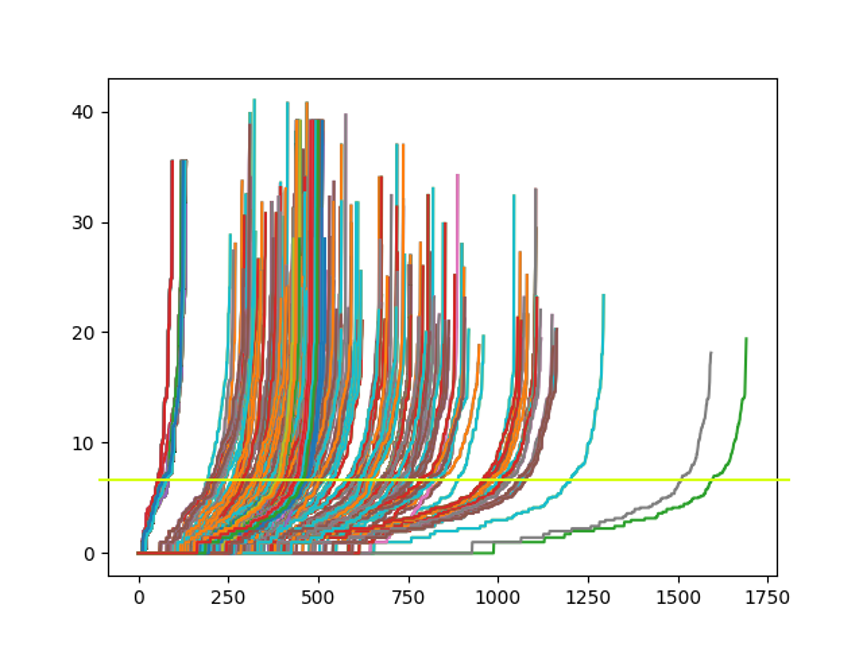
\includegraphics[width=\linewidth]{chapters/6/img/kmembersgraph.png}
\caption{K-nearest neighbors graph generated for packets in the dataset using a \texttt{min\_samples} = 6}
\label{fig:kneighborsgraph}
\end{figure}

\subsection{Packet Classification}
For deep learning, we feed the extracted cluster features forward into a two-layer multilayer perceptron unit (MLP) with a final softmax layer for classification. We use binary cross entropy as the loss function.

\section{Experiments and Results}

We experimented with the RTP detection problem that was previously attempted with the \textsc{Maple} model in chapter 5 in order to assess the ability to detect weakly signatured data. Then, we extend this to H.225 detection, which is another data transfer protocol with a weak signature. Lastly, the model performance and throughput is assessed for its application to deep packet inspection and deep learning at scale.

All tests were performed on a single CPU of a 1.6 GHz dual-core Intel i5 processor with 16 GB DDR3 RAM. In the binary confusion matrix, true positive (TP) indicates correct classification of data as RTP. True negative (TN) is correct classification of data as non-RTP. false negative (FN) implies incorrect identification of traffic as non-RTP, and false positive (FP) is the incorrect classification of data as RTP. We use measurements of precision, recall, and F1-score for model evaluation, defined as follows:
\begin{equation}
\begin{split}
    Recall = \frac{TP}{TP + FP} \text{  }
    Precision = \frac{TP}{TP + FN} \\
    F1\text{ }Score = \frac{2(P\times R)}{P + R} \\
    \end{split}
\end{equation}

All tests were performed with undersampling to appropriately balance the dataset, and a 60\%/40\% training and test split. Epochs represent the number of passes made over the training data in order for the neural network to fine tune itself under supervision. Although more epochs do not guarantee better performance, it is often the case that a larger number of epochs within reason can improve metric results. However, too many epochs can cause overfitting to the training data and hurt generalizability.

\subsection{RTP Detection}
Our primary goal in designing \textsc{Date} was to capture spatial hidden representaitons which may be present in these geometric reinterpretations of packets. These features may present advantage to our classifier as dynamic ports and weak signatures found in these protocols make traditional signature-based and port-based methods ineffective. The classification results of the \textsc{Date} model are provided in Table~\ref{tab:rtpresults}. Table~\ref{tab:rtpresultslsh} show the combined \textsc{Alpine} and \textsc{Palm} technique's results for the RTP classification task. There is clear improvement for the \textsc{Date} model.

\begin{table} [h!]
\centering
\begin{tabular}{| r | c | c | c |}
\hline
Class & P & R & F1 \\
\hline
\textit{Non-RTP} & 0.73 & 0.77 & 0.75 \\
\textit{RTP} & 0.76 & 0.71 & 0.73 \\
\hline
\end{tabular}
\caption{Classification results of RTP vs non-RTP detection for \textsc{Alpine} and \textsc{Palm}}
\label{tab:rtpresultslsh}
\end{table}

\begin{table} [h!]
\centering
\begin{tabular}{| r | c | c | c |}
\hline
Class & P & R & F1 \\
\hline
\textbf{1 Epoch} &&& \\
\textit{Non-RTP} & 0.85 & 0.84 & 0.84 \\
\textit{RTP} & 0.83 & 0.85 & 0.84 \\
\hline
\textbf{10 Epochs} &&& \\
\textit{Non-RTP} & 0.94 & 0.81 & 0.87 \\
\textit{RTP} & 0.83 & 0.95 & 0.89 \\
\hline
\textbf{20 Epochs} &&& \\
\textit{Non-RTP} & 0.96 & 0.79 & 0.87 \\
\textit{RTP} & 0.82 & 0.96 & 0.89 \\
\hline
\end{tabular}
\caption{Classification results of RTP vs non-RTP detection for the \textsc{Date} model}
\label{tab:rtpresults}
\end{table}

\subsection{H.225 Detection}
H.225 handles the registration and call setup for certain VoIP architectures using the H.323 protocol suite. Similar to RTP, H.225 data can arrive at the endpoint first before H.323 which it must be paired with. It also does not have a strong signature. Thus, we additionally tested \textsc{Date}'s ability to detect H.225 traffic from non-H.225 traffic. Our setup of the dataset labels and the DBSCAN configuration was similar to the RTP test and results are given in Table~\ref{tab:h225results}. The performance of \textsc{Alpine} and \textsc{Palm} are provided in Table~\ref{tab:h225resultslsh} for a baseline.

\begin{table} [h!]
\centering
\begin{tabular}{| r | c | c | c |}
\hline
Class & P & R & F1 \\
\hline
\textit{Non-H.225} & 0.62 & 0.64 & 0.63 \\
\textit{H.225} & 0.63 & 0.61 & 0.62 \\
\hline
\end{tabular}
\caption{Classification results of H.225 vs non-H.225 detection for
\textsc{Alpine} and \textsc{Palm}}
\label{tab:h225resultslsh}
\end{table}


\begin{table} [h!]
\centering
\begin{tabular}{| r | c | c | c |}
\hline
Class & P & R & F1 \\
\hline
\textbf{1 Epoch} &&& \\
\textit{Non-H.225} & 0.98 & 0.83 & 0.90 \\
\textit{H.225} & 0.85 & 0.99 & 0.92 \\
\hline
\textbf{10 Epochs} &&& \\
\textit{Non-H.225} & 0.91 & 0.87 & 0.89 \\
\textit{H.225} & 0.88 & 0.92 & 0.90 \\
\hline
\textbf{20 Epochs} &&& \\
\textit{Non-H.225} & 0.98 & 0.83 & 0.90 \\
\textit{H.225} & 0.85 & 0.99 & 0.92 \\
\hline
\end{tabular}
\caption{Classification results of H.225 vs non-H.225 detection for the \textsc{Date} model}
\label{tab:h225results}
\end{table}

\subsection{Model Performance and Throughput}
In order to benchmark the system for real deployment, we recorded the time classification took. While this is heavily system dependent and showed some variance across parameter tuning or model configuration, the average classification time for a single packet by \textsc{DATE} was 0.15823 seconds.

\section{Discussion and Limitations}

Of the models tested so far in this work, \textsc{Date} is the most computationally complex with the lowest throughput. In future work, we propose implementing multi-threading and multi-core processing as potential optimizations. We observed that point cloud generation was a pain point for the system in terms of cycles, and consider offloading such repetitive calculations to a specialized hardware such as FPGA~\cite{Song2005EfficientPC} when available in the deployed system. Because \textsc{Maple} is able to normalize data and map it into a three-dimensional cluster space, it would be well-suited to heterogeneous data such as sensor data combined with packet data from an internet of things device. This would create a multi-embedding capable of correlating these data inputs for machine learning tasks. Simpler problems may be solved with more naïve approaches such as regular expression matching on plaintext SIP traffic, or using the locality-sensitive hashing strategy toward device fingerprinting.

We propose both \textsc{Maple} and \textsc{Date} as potential methods for generating hidden, latent-space representations of traffic as their capabilities extend to different problem areas. \textsc{Maple} works well on input data such as a payload which may be distinct one data sample from another, but can be divided and matricized into units for comparison (i.e. turned into a grayscale image of uniform dimension). On the other hand, \textsc{Date} has the potential to expand to include other non-network features and represent more heterogenous data. For example, input sensor data from IoT devices or light detection and ranging (LiDAR) equipment have used DBSCAN for data processing and normalization~\cite{wanglidar2019}; it could be combined with cloud/network data inputs as an additional embedding model for classification problems. While for the RTP problem \textsc{Maple} provides high accuracy with more efficiency than \textsc{Date}, there is a trade-off within the embedding space as \textsc{Date} may be able to represent data of higher complexity in other problems for future work.


\chapter{FORAGER - TOWARDS MULTI-EMBEDDINGS AND ENSEMBLE CLASSIFICATION}
\section{Introduction}

In the previous work with \textsc{Alpine} and \textsc{Palm} we hypothesized that enabling both models to run together and combine their votes would yield the most accurate and agreed-upon classification results. The results of the multi-embedding experiments in this work proved this to be more accurate. Multiple classifier systems (MCS) are ensembles and are widely used in pattern recognition applications and recognized as more effective than any single embedding or classifier. There are at least three reasons identified by Dietterich as to why multi-classifier approaches perform well~\cite{dietterich2000ensemble}:

\begin{itemize}
    \item Statistically, there is a set of $H$ hypotheses for which the learning algorithm is performing a search for the best hypothesis. The risk of choosing the wrong classifier is reduced when using multiple for unseen data.
    \item Computationally, optimal training is an NP-hard problem. Because the optimum depends on the starting point, the optimal learning algorithm may be different. By using an ensemble, a better approximation of the unknown function may be obtained.
    \item Representationally, the weighted sums of hypotheses from $H$ allows for the expanding of space of representable functions. Simply put, the more embeddings we have, the more features, and the more ways to represent and compare data.
\end{itemize}

In addition to multiple classifiers, in the workflow process using multiple types of embeddings has proven more effective in several recent, real systems than any single approach~\cite{tajaddodianfar2020texception, instruction2vec, duarte2019semi, yang2022, ayoade2020evolving, palau2020dns, kishioka2018, Boyaci2022, glass}.

As we have seen in previous chapters, each model unveils different hidden representations which are appropriate for different classification problems and contexts. In the real network environment, these classification problems are not isolated. Traffic may need to be distinguished between encrypted and plaintext, for example, and then protocols identified. Then, encrypted traffic may be profiled, or the plaintext traffic characterized by embedding for user fingerprints. Thus, a combined approach or toolkit is apt for the many kinds of problems real world network analysts face.

To meet this need, we propose \textsc{Forager}, a combination of data mining and hidden representation learning approaches to deep packet inspection and network traffic classification. This highly configurable toolkit includes the ability to extract and transform header features into locality-sensitive hashes indexed in an LSHForest using the \textsc{Alpine} technique. Payloads may be combinatorally analyzed using either the \textsc{Palm}, \textsc{Maple}, or \textsc{Date} approaches, or a combination of votes from these models. By considering the data from multiple angles, we achieve results of higher accuracy and a much greater understanding of the network traffic than other state-of-the-art systems.

To illustrate the capability of \textsc{Forager} and its diversity of traffic applications, we performed a case study on profiling the traffic on port 443. Due to the rise of encryption and its standard usage for Hypertext Transfer Protocol Secure (HTTPS) encrypted traffic, port 443 is often left un-monitored by packet inspection on large-scale surveillance systems or default-allowed by firewall software. While the majority of internet traffic is now safely secured behind transport layer security, there are threat actors who have found ways to utilize port 443 as a covert data channel for surveillance and firewall evasion, malware transport, data exfiltration, and nefarious activity under the guise of internet anonymity. For increased security and surveillance, it is necessary to be able to filter legitimate, HTTPS traffic from illicit activity on this port. We propose using \textsc{Forager}, our network traffic classification and profiling toolkit, to dissect this traffic stream for hidden content. Using \textsc{Forager} and its individual models, we are able to extract plaintext and compressed traffic from encrypted streams with high accuracy, profile Tor-based, VPN-based, and encrypted traffic streams by application and data type, and identify malicious instances of particular protocols designated to run over HTTPS. Our models combine several approaches to hidden feature extraction from packets via spatial representation learning to precisely and efficiently classify packets, fortifying network security while still preserving user privacy through this crucial gateway.

\section{Previous Work}

In our threat model and in the works we compare against~\cite{choorod2022tor, didarknet, deeppacket}, we choose to prioritize making classification using only a single packet from any point in the overall traffic flow. This contrasts systems which require entire flows in order to classify~\cite{perera2017comparison, deeppacket, panchenko2011website, amaral2016machine, cao2014survey}.

\subsection{VPN Traffic Profiling}
Deep Packet~\cite{deeppacket} uses a CNN to perform traffic classification into traffic types and application types as labeled in the VPN/non-VPN UNB ISCX dataset~\cite{vpn-dataset}. Their solution achieves 94\% accuracy classifying traffic by type, and 97\% accuracy in classifying by application. Like our work, they use a single packet in the classification task, and do not rely on flow-based features. We note that their work does not perform as well in Tor traffic classification, leading us to conclude that Deep Packet may not generalize as well as \textsc{Forager}. Cui et al use only header information from the ISCX datasets to classify traffic over flows with 99\% accuracy~\cite{onlyheader}. While a novel solution with enhanced privacy as it considers only header features, it still requires flow-based features of the header and therefore multiple packets. Zou et al use the spatial features of the first packet of a flow extracted and applied to a CNN and analyze the time series features of the next three packets using a long short-term memory network (LSTM)~\cite{zhou2018encrypted}. This method shows high accuracy on the dataset but requires flow-based information.

\subsection{Darknet Detection and Profiling}

Lotfollahi et al also study the ISCX dataset for Tor data and profile again by application and traffic type using a single packet approach~\cite{deeppacket}. Tor traffic profiling has been further explored by Lashkari et al~\cite{didarknet} in their DIDarknet system using a single packet, where they also proved accurate results using the ISCX Tor dataset. Other works have used flow-based features for both detecting Darknet activity (binary Tor/non-Tor classification) and profiling Tor traffic into specific applications or traffic types (e.g. streaming, chat, web browsing). Iliadis et al~\cite{iliadis2021darknet} use an amalgamated version of the ISCX Tor and VPN datasets, re-labeled CICDarknet2020, in order to create a binary classification of Darknet and regular traffic, and a multi-class problem of Tor, non-Tor, VPN, and non-VPN. We perform a similar analysis in our experiments and results of the same data. The work uses all 85 features published in the dataset, including flow-based features, and the full traffic information. Using a set of machine learning algorithms, they are able to achieve up to 98\% accuracy; however, in comparison our system uses only a single packet and a minimal set of features to achieve similar results. Ma et al~\cite{Ma2021dark} also achieved noted success in the community classifying the same dataset using a CNN with Root Mean Square (RMS) propagation. They also require flow-based features of the dataset, and would therefore require multiple packets and flow information in a real system. They also only consider Darknet detection without additional profiling and achieve 95\% accuracy, lower than ours in the same task. Sarkar et al~\cite{sarkar2020detection} introduce a Generative Adversarial Network (GAN) in order to stabilize their deep learning model across the same ISCX Tor dataset, and achieve approximately 98\% accuracy, as well. Using flow-based features, they are able to provide a 95\% accuracy in the profiling task across the eight described traffic classes in the dataset; however, they do not provide the results broken down individually so it is difficult to conclude if the model performs evenly well across classes or not. Choorod et al~\cite{choorod2022tor} use a statistical analysis solely of the extracted features of the encrypted packet payload. They find that certain sizes are common across traffic types, as well as certain regions of the encrypted payload. They use Charcount from the Posit Text Profiling Toolset~\cite{Weir2007ThePT} as a ratio value for input to their decision tree-based algorithm. They achieve highly accurate results we compare against in the Experiments section of this work.

\subsection{Filtering Compressed/Plaintext Traffic}
Plaintext filtering can be done through statistical entropy tests~\cite{wood2017cleartext} and has been used to find private medical or geo-location data~\cite{wood2017cleartext, Shbair2020ASO}, covert malware~\cite{singh2021comparative}, and general unencrypted traffic like file transfers or emails. Modern compression and encryption algorithms present such similar high entropy that distinguishing between them is a difficult problem. The HEDGE~\cite{hedge} system is able to parse encrypted from compressed traffic with between 60-94\% accuracy using the Chi Square and a subset of the NIST SP 800-22 tests dependent upon the size of the packet used. They compare against Hahn et al, who achieved a maximum of 66\% accuracy using machine learning models~\cite{Hahn2018DetectingCC}.

\subsection{Intrusion Detection over HTTPS}

Zain ul Abideen et al~\cite{abideen2019vpn} consider the problem of detecting and profiling VPN traffic on port 443, where their system uses non-encrypted, packet level features to determine several VPN types in the traffic flow. They distinguish between VPN configurations, including Tor. Furthermore, they employ a technique using DNS queries to identify malicious or illegitimate VPN servers. This is an interesting notion which may be challenged by the increased use of encrypted DNS and techniques like DNS-over-HTTPS. Identification of SSH flows in encrypted traffic has been accomplished with success when using flow data~\cite{Hellemons2012SSHCureAF}. Detecting brute-force and dictionary attacks over SSH is also a research problem area from which our work on port 443 is inspired~\cite{Ghitte2019FingerprintingTU}.

\section{Methodology}
Details of the network traffic classification systems used in Forager can be found in previous chapters of this work. In addition to technical methods, we provide practical application through analysis of threat models for which \textsc{Forager} is useful.

\subsection{Threat Model}
To bring the problem to life, we envision a criminal case in our \textit{\textbf{threat model}}. Bob is a member of an organization embezzling funds through an international shipping company. There are several nefarious tasks which Bob needs to accomplish that he could utilize port 443 exploitations to achieve:
\begin{itemize}
\item Create a \textbf{\textit{covert data channel}} in order to pass along sensitive information like receipts and records while avoiding detection,
\item \textbf{\textit{Communicate anonymously}} with criminal network colleagues to avoid tracing of colleagues, his own geolocation data, and evidence,
\item Establish \textbf{\textit{remote access}} to a machine from endpoints configured to disallow ports like 22,
\item \textbf{\textit{Exfiltrate data}} from a secure source.
\end{itemize}

Alice is an intelligence officer who is monitoring Bob's network data with reasonable suspicion that he is engaged in criminal acts. We will discuss vulnerabilities in Alice's current surveillance framework and how to use \textsc{Forager} to capture and record evidence which can be used to thwart Bob's plans and provide legal support in the case against his embezzlement and fraudulent company.

\subsubsection{Real-Time Monitoring}

In our scenario, Alice possesses a middlebox technology configured to monitor traffic on port 443. It is common for routers or middleboxes to default-ignore traffic on port 443 as there is usually an overwhelming amount of encrypted traffic on this port that is unprocessable~\cite{shane-review-dns-over-http-04}. Attackers who are aware of this strategy may send unencrypted or sensitive information over port 443 in order to avoid surveillance and detection. In criminal operations, these packets could contain significant data. Thus, it is important for middlebox technologies to have a methodology for scanning traffic on port 443 to determine if the data is truly encrypted. If the data is plaintext, it may be directly processed. If it is highly entropic but only compressed, follow-on processing may be capable of decompressing the data. Currently, Alice configures her middlebox to default-ignore traffic on port 443, instead only monitoring port 143 for unencrypted emails. In order to avoid detection by possible surveillance technology, Bob routes his emails through port 443. The receiver is aware of this and listens for this traffic with the IMAP server on the configured port so that it is received. Thus, Bob is able to transmit content in a way that is receivable by the partner as email/IMAP at no additional security overhead but is undetected as Alice's middlebox does not scan port 443.

\subsubsection{Tunnel Tracking}
Tor allows anonymous Internet space for pervasive action and may be used to access content which is blocked by firewalls, whether it be censored or illegal activity. While possibly encrypted and encapsulated with layers of addressing in order to anonymize routing, traffic may be synchronized by timing and further analysis in order to determine endpoints~\cite{Simioni2021}. Thus, tracking Tor and being able to further profile Tor usage and content is a useful operation for intelligence and law enforcement. Network Address Translation (NAT) in VPNs prevents traditional ISP tracking. The ability to detect VPN traffic streams and profile their traffic and applications can be additionally useful for network monitoring. In the scenario, Bob is using a VPN to connect to a forum website. He wishes to remain anonymous during this communication. Alice is following Bob's messages, and sees that he regularly communicates using HTTP and IRC protocols on this platform. She configures her middlebox device to promote traffic on several five-tuple-based traffic flows which she knows to be currently associated with Bob's devices. However, dynamic re-configuration of the tunneled network layers causes Alice to lose the data stream and she is no longer able to monitor his messages and record the activity.

\begin{figure} [ht!]
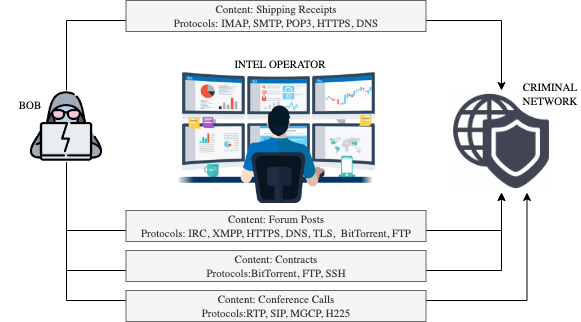
\includegraphics[width=\linewidth]{chapters/7/img/attackscenarios.drawio.png}
\caption{A depiction of intelligence operations intercepting various types of traffic Bob is transmitting in connection to his extended criminal network.}
\label{fig:attacks}
\end{figure}

\subsubsection{Covert Data Channels In}
Domain name security (DNS) has long been exploited by attackers due to many security loopholes and its historical transmission in plaintext. Malicious actors may embed malware or sensitive data into DNS records~\cite{iscx-doh-paper}. This becomes even harder to detect when the tunnel is then encrypted, as is the case with DNS over HTTPS~\cite{rfc8484}. Since its inception, DNS over HTTPS has been adopted by mainstream browsers like Firefox and Chrome to prevent man-in-the-middle attacks and snooping on DNS traffic. While enhancing user privacy, this has contraversely become a field of opportunity for cyber attackers as DNS traffic that is now encrypted may bypass traditional DNS security systems. Thus, the DNS-over-HTTPS (DoH) pipeline can become both a covert channel for malware entering systems as well as data being exfiltrated out. For example, in 2020 the Iranian threat actor group APT34 used DNSExfiltrator2, an open-source DoH tool, to laterally move data to their networks~\cite{quointelligence-apt34}. Malware such as Godlua~\cite{trendmicro-godlua} and PsiXBot~\cite{proofpoint} have also been spotted in the wild along DoH channels. As an example in our scenario, imagine Bob wants to track activity or exfiltrate data from a server in a competitor's private network. In order to record this information, he needs to plant a trojan virus on this server. Using DNS-over-HTTPS as a covert data channel, Bob hosts the trojan on a website and uses social engineering to engage a user to click a link, querying the domain and returning the data which contains the trojan. This malware remains undetected as port 443 traffic is not scanned.

\subsubsection{Covert Data Channels Out}
Many enterprise network environments restrict outbound traffic to ports 80 and 443. Users may re-reroute DNS from the standard port 53 to avoid defeat by firewalls, ISPs, or government or enterprise networks~\cite{shane-review-dns-over-http-04}. Similarly, firewalls can also be bypassed using SSH over port 443. SSH, or secure shell protocol, gives users a method of accessing another computer over an insecure network. While typically transmitted over port 22, many firewalls default to defeating traffic over this port. Instead, they allow traffic over port 443. Packages exist such as \texttt{stunnel} which make SSH tunneling over 443 simple for any Internet user~\cite{wong2001stunnel}. Creating a covert data channel over SSH can also be a gateway for cache attacks as it is necessary to transmit or exfiltrate the data when accessed~\cite{Maurice2017HelloFT}. In our scenario, Alice's middlebox technology is monitoring traffic on port 22 (SSH) for secure shell sessions. Bob needs to SSH into a machine and copy over some documents. Instead of relying on traditional channels, Bob has re-routed his SSH connection through port 443, creating a covert data channel. Thus, Alice is missing the mission critical data of the file transfer.

\subsection{System Design}

The \textsc{Forager} system is a highly adaptable traffic profiling multi-tool capable of representing packets in multi-dimensional space through configurable modules. Users can enable up to four different methods of latent representation for the packets. Each of these modules assesses different portions of the packet data with various hidden representation learning approaches. Specifically, \textsc{Alpine} and \textsc{Palm}~\cite{kapoor2022deep} generate one-dimensional locality sensitive hashes which represents single sets of features from the header and payload. \textsc{Maple} and \textsc{Date} generate two-dimensional images and three-dimensional point clouds with clusters, respectively. Votes are provided to the overall framework and used in lookup to generate a classification report. The whole system is depicted in Figure~\ref{fig:forager}.

\begin{figure} [ht!]
\centering
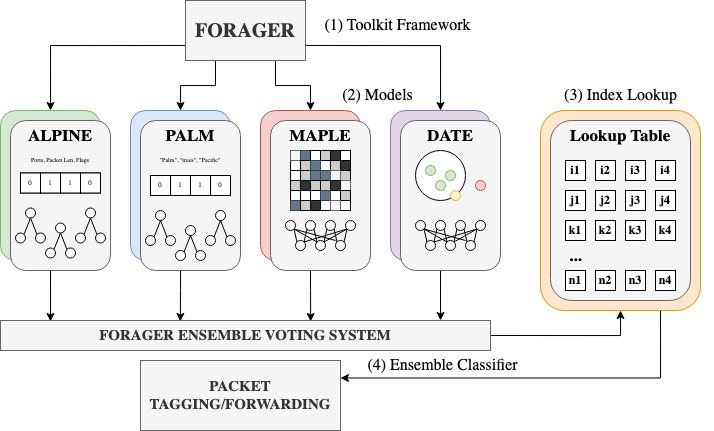
\includegraphics[scale=0.5]{chapters/7/img/forager.png}
\caption{System diagram of \textsc{Forager}.}
\label{fig:forager}
\end{figure}

In the training phase, data is passed in with a label and indexed respective to class. This index is stored in a lookup table inside \textsc{Forager}. Models are enabled or disabled and given a number of votes $m$ per model. This allows the user to more heavily weight one model's opinion over another, further contributing to the flexibility in real deployments. A few additional hyperparameters may be configured for the neural network models such as epochs for training, and data is processed and weights may be saved for later use. In the testing phase, test data is processed in a similar manner and the input passed through the classifier. \textsc{Date} amalgamates the votes across models and uses its lookup table to return a classification result. In a real packet processing pipeline, we could add this result as part of metadata or an encapsulation header for the packet for downstream processing. The current implementation generates a report of classification results which may be returned to an administrator for further review and possible identification of traffic on non-standard or unexpected ports which could be malicious.

\subsection{Datasets}
To create a pipeline of data representative of a diverse capture on port 443, we utilized several public datasets created by and widely used in the research community for network traffic classification.

\subsubsection{ISCX 2016 VPN-nonVPN Dataset}
We used the UNB ISCX 2016 VPN-nonVPN dataset~\cite{vpn-dataset}. This dataset is a real-world simulation capture created by the Canadian Institute for Cybersecurity (CIC) specifically for encrypted VPN traffic classification~\cite{iscx-vpn-paper}. The traffic was captured using Wireshark and tcpdump and generated using OpenVPN; it contains 28GB of traffic. The packets are a mixture of encrypted and compressed or plaintext traffic. Because these are real-world captures, there are some packets such as ICMP and ARP which are service-level and irrelevant for application and traffic type classification. For this reason, we discard non-TCP/UDP packets as part of the process. Previous work~\cite{deeppacket, Zhou2020, Song2019} in machine learning-based traffic classification has made use of this public dataset and made similar modifications. A breakdown of the dataset is provided in Table~\ref{tab:iscxvpndetails}. The data is divided into the following categories:
\begin{itemize}
    \item \textit{Traffic Type} - There are seven types of traffic: Browsing, File Transfer, Email, Chat, Streaming, VoIP, and P2P.
    \item \textit{Application} - Several of the PCAPs were associated specifically with one application such as Skype or Google Hangouts. The applications we uniquely identify are Pidgin (IAM and ICQ chat), BitTorrent (P2P), Facebook, Skype, Google Hangouts, Spotify, Vimeo, Youtube, Netflix, Thunderbird (Email), and Filezilla (FTP).
\end{itemize}

\begin{table} [ht!]
  \centering
  \begin{tabular}{|p{3cm}|p{8cm}|}
   \hline
   \textbf{Traffic} & \textbf{Content} \\
   \hline
   Browsing & Firefox and Chrome\\
   Email & SMTPS, POP3S and IMAPS\\
   Chat & ICQ, AIM, Skype, Facebook, Hangouts\\
   Streaming & Vimeo, Youtube, Spotify\\
   File Transfer & Skype, FTPS and SFTP using Filezilla\\
   VoIP & Facebook, Skype, Hangouts voice calls\\
   P2P & uTorrent, BitTorrent, Vuze\\
  \hline
  \end{tabular}
  \newline
  \vspace*{0.25 cm}
  \newline
  \begin{tabular}{| c | c | c | c |}
  \hline
   \textbf{Application} & \textbf{Benign} & \textbf{VPN} & \textbf{Tor} \\
   \hline
   AIM chat & 6K & 1.4K & 2K \\
   Email & 50K & 25K & 163K \\
   Facebook & 1837K & 36K & 88K \\
   Filezilla (FTPS) & 312K & 315K & 143K \\
   Filezilla (SFTP) & 629K & 182K & 176K \\
   Gmail & 15K & -- & -- \\
   Chrome & -- & -- & 356K \\
   Hangouts & 1871K & 151K & 1114K \\
   Pidgin (ICQ) & 4K & 7K & 2K \\
   Netflix & 455K & 1433K & -- \\
   SCP & 777K & -- & -- \\
   Skype & 2261K & 1069K & 564K \\
   Spotify & 63K & 193K & 118K \\
   Bittorrent & -- & 133K & -- \\
   VoipBuster & 1017K & 823K & -- \\
   Vimeo & 214K & 591K & 288K \\
   Vuze & -- & -- & 264K \\
   Youtube & 377K & 333K & 261K \\
   \hline
   \end{tabular}
   \caption{ISCX VPN/non-VPN and Tor/non-Tor Datasets}
  \label{tab:iscxvpndetails}
\end{table}

\subsubsection{Tor Datasets}

The Canadian Institute for Cybersecurity similarly created the UNB ISCX 2016 Tor-nonTor~\cite{tor-dataset} dataset which captures data routed over Tor. The traffic was generated using Whonix~\footnote{https://www.whonix.org} and captured using Wireshark and tcpdump; the Tor dataset contains 22GB of traffic. The benign traffic used for comparison in their traffic profiling work~\cite{iscx-tor-paper} is the same from the VPN dataset, establishing a good baseline for our work in combining these two. A gateway was configured to convert non-encapsulated traffic into Tor PCAPs which were then routed to the Tor network. Because Tor is a circuit-oriented network, all traffic from the gateway to the entry node will be routed through the same connection~\cite{iscx-tor-paper} which could cause over-fitting to a particular dataset. In order to better simulate the diversity of network routing methods, we added as another Tor sample PCAPs from Skynet, a Tor-powered botnet with publicly available datasets for research purposes~\cite{skynet}. For a botnet, the advantage of Tor is hidden services. There is no way to trace the original IP address of a hidden server which is published with its .onion pseudo-domain. All botnet traffic is encrypted. The malware which infects the host opens a SOCKS proxy on port 55080 reachable through the .onion domain, and can then run a number of bundled attacks and operations like bitcoin mining, data exfiltration, and DDoS attacks~\cite{skynet}. Thus, we leverage evidence of this botnet implementation as an additional Tor data connection.

\subsubsection{CIRA-CIC-DoHBrw-2020 Dataset}
CIC has also made the CIRA-CIC-DoHBrw-2020 dataset containing DNS-over-HTTPS (DoH) and non-DoH traffic on port 443, with a secondary layer of benign versus malicious DoH traffic~\cite{iscx-doh-paper}. The traffic was generated by querying the top 10K Alexa websites. For non-DoH traffic, an HTTPS request is sent for the website with regular, plaintext DNS. Firefox and Chrome browsers with the configured DNS-over-HTTPS setting were used for benign DoH traffic. For each of the browsers, there were four DNS services used: Cloudflare, AdGuard, Google, and Quad9. Finally, for malicious DoH traffic, tunneling tools dns2tcp, DNSCat2 and Iodine were used to created encrypted TCP covert data channels for transmission. A domain and authoritative name server were established and the DoH tunneling tool used in the client/server interaction. The packet pre-processing we performed on this data was similar to the VPN and Tor dataset processing; a distribution of the data is provided in Table~\ref{tab:dohdataset}.

\subsubsection{EMews SoH Dataset}
SSH is another exploitable protocol for both malware injection and data exfiltration over HTTPS. In 2018, Ricks et al~\cite{Ricks2018ddos} created an SSH over HTTPS (SoH) simulation using the eMews framework and CORE to generate packet traces. The network consists of 1022 nodes, 36 of which incorporate the SSH sessions and the others perform various web-crawling activity for benign comparison. EMews~\footnote{https://mews.sv.cmu.edu/research/emews/} itself is an open-source, large-scale network traffic data generation tool designed to emulate networks employing protocols which require human interaction (ex: starting an SSH connection). Sample counts for this dataset are provided in Table~\ref{tab:sohdataset}.

\begin{table} [ht!]
{
  \centering
  \begin{tabular}{|c|c|c|}
   \hline
   \textbf{Classification} & \textbf{Application} & \textbf{Sample Count} \\
   \hline
   \textit{non-DoH} & Chrome & 542K \\
    & Firefox & 356K \\
   \hline
   \textit{Benign DoH} & Chrome & 3.5K \\
    & Firefox & 16.2K \\
   \hline
   \textit{Malicious DoH} & dns2tcp & 168K \\
   & DNSCat2 & 36K \\
   & Iodine & 47K \\
   \hline
   \end{tabular}
  \caption{Summary of CIRA-CIC-DoHBrw-2020 Dataset}
  \label{tab:dohdataset}
}
\end{table}

\begin{table} [ht!]
{
  \centering
  \begin{tabular}{|c|c|}
   \hline
   \textbf{Classification} & \textbf{Sample Count} \\
   \hline
   HTTPS & 542K \\
   SSH over HTTPS & 3.5K \\
   \hline
   \end{tabular}
  \caption{Summary of eMews SSH over HTTPS Dataset}
  \label{tab:sohdataset}
}
\end{table}

\section{Experiments and Results}

We use measures of precision, recall, and F1 score for classifier assessment. In the binary confusion matrix, true positive (TP) indicates correct classification of data as some protocol class $C$. True negative (TN) is correct classification of data as \textit{not} class $C$. false negative (FN) implies incorrect identification of traffic as not $C$, and false positive (FP) is the incorrect classification of data as $C$.
\begin{equation}
\begin{split}
    R(C) = \frac{TP}{TP + FP} \text{,  }
    P(C) = \frac{TP}{TP + FN} \text{,  }
    F1(C) = \frac{2(P\times R)}{P + R} \\
    \end{split}
\end{equation}

A high recall indicates that in the binary problem, much of the traffic is correctly identified as the positive class. High precision in the model shows the quality of positive classifications, i.e. indicates how many were correctly classified out of everything said to be in the positive class. A model with low recall and high precision will likely mis-classify traffic which does belong in the positive class (high rate of false negatives), whereas a model with high recall and low precision will produce more false positives. In the following scenarios, we analyzed different potential traffic classification problems for port 443 based on the described attacks or opportunities from the threat models.

\subsection{VPN Traffic Profiling}

We analyzed the ISCX VPN/non-VPN dataset according to the applications and traffic types identified by the researchers who generated the data and Lotfollahi et al~\cite{deeppacket} who used the same data for per-packet classification in their Deep Packet models. They used a convolutional neural network and stacked autencoder model for implementations. We used three different configurations of \textsc{Forager} for the traffic and application classification tasks. For each problem, we ran a combination of \textsc{Alpine} and one of the payload transformation models. For application classification, DeepPacket's CNN model achieved very high F1 scores for most of the applications. Overall, each model is quite successful in distinguishing applications without inspecting packet contents, preserving user privacy while still accomplishing the mission. In the threat model, Alice could use our tool to better understand what kind of Internet behavior Bob is engaging in over his VPN connection. We notice in both application and traffic classification tasks, our \textsc{Forager} models achieve some improved results in the VoIP categories. Our models also perform significantly better in profiling the benign/non-VPN traffic types, up to 0.13 higher than the stacked auto encoder in the VoIP category as well. When ICQ and AIM were combined under the Chat category, \textsc{Forager} achieves much higher results than any other model. For all models, distinguishing ICQ and AIM traffic was a difficult task. In further investigation into the network environment, we found both of these traffic streams were generated from the Pidgin messaging application, which makes sense that they were misclassified as one another in all the models. We also note that apps which use similar protocol stacks or likely similar APIs tend to be misclassified as one another. for example, FTPS and SFTP (both using FTP) are more difficult to distinguish from one another than either against SCP using SSH~\cite{deeppacket}. This is an important note for training and defining classes for neural network models in general, as well-defined classes or clusters make classification a clearer task. One significant difference in the experimental setup of Deep Packet versus \textsc{Forager} is that DeepPacket's CNN requires 300 epochs to train the entire network. \textsc{Maple} achieves near comparable results at a mere 10 epochs of training on the same data and split. \textsc{Date} also achieves good results only training with 10 epochs on its statistical model. We ran additional tests, increasing the number of epochs in order to determine if this improved our models' efficacy. In each case, 10 epochs proved to be sufficient for training \textsc{Forager} to maximum performance capability.

\begin{table*} [ht!]
\resizebox{\textwidth}{!}{\begin{tabular} {|p{2.3cm}|p{2.2cm}|p{2cm}|p{2cm}|p{2cm}|p{2cm}|}
\hline
\textbf{Application} & DeepPacket-CNN & DeepPacket-SAE & \textsc{Alpine} + \textsc{Palm} & \textsc{Alpine} + \textsc{Maple} & \textsc{Alpine} + \textsc{Date} \\
\hline
\end{tabular}}
\resizebox{\textwidth}{!}{\begin{tabular} {|p{2cm}|p{0.7cm}p{0.7cm}p{0.7cm}|p{0.7cm}p{0.7cm}p{0.7cm}|p{0.7cm}p{0.7cm}p{0.7cm}|p{0.7cm}p{0.7cm}p{0.7cm}|p{0.7cm}p{0.7cm}p{0.7cm}|}
\hline
& \textit{P} & \textit{R} & \textit{F1} & \textit{P} & \textit{R} & \textit{F1} & \textit{P} & \textit{R} & %
\textit{F1} & \textit{P} & \textit{R} & \textit{F1} & \textit{P} & \textit{R} & \textit{F1} \\
\hline
AIM chat & 0.87 & 0.76 & \textbf{0.81} & 0.76 & 0.64 & 0.70 & 0.80 & 0.55 & 0.65 & 0.80 & 0.57 & 0.67 & 0.67 & 0.69 & 0.68 \\
Email & 0.97 & 0.82 & 0.89 & 0.94 & 0.99 & \textbf{0.97} & 0.81 & 0.76 & 0.79 & 0.74 & 0.80 & 0.77 & 0.86 & 0.73 & 0.79 \\
Facebook & 0.96 & 0.95 & \textbf{0.96} & 0.94 & 0.95 & 0.95 & 0.96 & 0.90 & 0.93 & 0.97 & 0.91 & 0.94 & 0.98 & 0.90 & 0.94 \\
FTPS & 1.00 & 1.00 & \textbf{1.00} & 0.97 & 0.77 & 0.86 & 1.00 & 0.98 & 0.99 & 0.99 & 0.99 & 0.99 & 0.99 & 0.99 & 0.99 \\
Gmail & 0.97 & 0.95 & \textbf{0.96} & 0.93 & 0.94 & 0.94 & 0.96 & 0.87 & 0.91 & 0.94 & 0.90 & 0.92 & 0.95 & 0.90 & 0.92 \\
Hangouts & 0.96 & 0.98 & \textbf{0.97} & 0.94 & 0.99 & 0.97 & 0.98 & 0.89 & 0.93 & 0.96 & 0.91 & 0.94 & 0.96 & 0.91 & 0.94 \\
ICQ & 0.72 & 0.80 & \textbf{0.76} & 0.69 & 0.69 & 0.69 & 0.47 & 0.93 & 0.63 & 0.59 & 0.89 & 0.71 & 0.60 & 0.89 & 0.72 \\
Netflix & 1.00 & 1.00 & \textbf{1.00} & 1.00 & 1.00 & 1.00 & 0.99 & 0.98 & 0.99 & 0.99 & 0.99 & 0.99 & 0.99 & 0.99 & 0.99 \\
SCP & 0.97 & 0.99 & 0.98 & 1.00 & 1.00 & \textbf{1.00} & 0.98 & 0.91 & 0.94 & 0.98 & 0.92 & 0.95 & 0.97 & 0.91 & 0.94 \\
SFTP & 1.00 & 1.00 & \textbf{1.00} & 0.70 & 0.96 & 0.81 & 0.99 & 1.00 & 1.00 & 0.99 & 1.00 & 0.99 & 0.99 & 1.00 & 1.00 \\
Skype & 0.94 & 0.99 & 0.97 & 0.95 & 0.93 & 0.94 & 0.99 & 0.95 & \textbf{0.97} & 0.98 & 0.92 & 0.95 & 0.98 & 0.92 & 0.95 \\
Spotify & 0.98 & 0.98 & \textbf{0.98} & 0.98 & 0.98 & 0.98 & 0.99 & 0.92 & 0.95 & 0.99 & 0.95 & 0.97 & 0.99 & 0.95 & 0.97 \\
Torrent & 1.00 & 1.00 & \textbf{1.00} & 1.00 & 1.00 & 1.00 & 0.99 & 0.97 & 0.98 & 0.98 & 0.99 & 0.98 & 0.98 & 0.99 & 0.98 \\
VoipBuster & 0.99 & 1.00 & 0.99 & 0.99 & 0.99 & 0.99 & 1.00 & 0.98 & 0.99 & 1.00 & 0.98 & 0.99 & 1.00 & 0.99 & \textbf{0.99} \\
Vimeo & 0.99 & 0.99 & \textbf{0.99} & 0.99 & 0.98 & 0.98 & 0.99 & 0.98 & 0.99 & 0.97 & 0.98 & 0.99 & 0.98 & 0.98 & 0.98 \\
Youtube & 0.99 & 0.99 & \textbf{0.99} & 0.98 & 0.99 & 0.99 & 0.99 & 0.94 & 0.96 & 0.96 & 0.96 & 0.96 & 0.96 & 0.96 & 0.96 \\
\hline
\end{tabular}}
\resizebox{\textwidth}{!}{\begin{tabular} {|p{2cm}|p{2.3cm}|p{2.4cm}|p{2.3cm}|p{2.4cm}|p{2.3cm}|}
\hline
\textbf{Traffic Type} & DeepPacket-CNN & DeepPacket-SAE & \textsc{Alpine} + \textsc{Palm} & \textsc{Alpine} + \textsc{Maple} & \textsc{Alpine} + \textsc{Date} \\
\hline
\end{tabular}}
\resizebox{\textwidth}{!}{\begin{tabular} {|p{2cm}|p{0.7cm}p{0.7cm}p{0.7cm}|p{0.7cm}p{0.7cm}p{0.7cm}|p{0.7cm}p{0.7cm}p{0.7cm}|p{0.7cm}p{0.7cm}p{0.7cm}|p{0.7cm}p{0.7cm}p{0.7cm}|}
\hline
& \textit{P} & \textit{R} & \textit{F1} & \textit{P} & \textit{R} & \textit{F1} & \textit{P} & \textit{R} & %
\textit{F1} & \textit{P} & \textit{R} & \textit{F1} & \textit{P} & \textit{R} & \textit{F1} \\
\hline
Chat & 0.84 & 0.71 & 0.77 & 0.82 & 0.68 & 0.74 & 0.95 & 0.81 & \textbf{0.87} & 0.93 & 0.64 & 0.76 & 0.82 & 0.72 & 0.77 \\
Email & 0.96 & 0.87 & 0.91 & 0.97 & 0.93 & \textbf{0.95} & 0.76 & 0.99 & 0.86 & 0.71 & 0.74 & 0.73 & 0.75 & 0.67 & 0.71\\
File Transfer & 0.98 & 1.00 & \textbf{0.99} & 0.98 & 0.99 & \textbf{0.99} & 0.99 & 0.91 & 0.95 & 0.74 & 0.93 & 0.82 & 0.74 & 0.93 & 0.82 \\
Stream & 0.92 & 0.87 & 0.90 & 0.82 & 0.84 & 0.83 & 0.99 & 0.98 & \textbf{0.99} & 0.99 & 0.98 & \textbf{0.99} & 0.99 & 0.98 & \textbf{0.99} \\
VoIP & 0.63 & 0.88 & 0.74 & 0.64 & 0.90 & 0.75 & 0.99 & 0.95 & \textbf{0.97} & 0.99 & 0.94 & 0.96 & 0.99 & 0.95 & \textbf{0.97} \\
VPN: Chat & 0.98 & 0.98 & \textbf{0.98} & 0.95 & 0.94 & 0.94 & 0.96 & 0.95 & 0.96 & 0.96 & 0.98 & 0.97 & 0.96 & 0.97 & 0.97 \\
VPN: Transfer & 0.99 & 0.99 & \textbf{0.99} & 0.98 & 0.95 & 0.97 & 1.00 & 0.98 & \textbf{0.99} & 1.00 & 0.98 & \textbf{0.99} & 1.00 & 0.98 & \textbf{0.99} \\
VPN: Email & 0.99 & 0.98 & \textbf{0.99} & 0.97 & 0.93 & 0.95 & 1.00 & 0.98 & \textbf{0.99} & 0.99 & 0.98 & \textbf{0.99} & 0.97 & 0.99 & 0.98 \\
VPN: Stream & 1.00 & 1.00 & \textbf{1.00} & 0.99 & 0.99 & 0.99 & 0.99 & 0.99 & 0.99 & 0.99 & 0.99 & 0.99 & 0.99 & 0.80 & 0.89 \\
VPN: Torrent & 1.00 & 1.00 & \textbf{1.00} & 0.99 & 0.97 & 0.98 & 0.99 & 0.99 & 0.99 & 0.98 & 0.99 & 0.99 & 0.83 & 1.00 & 0.91 \\
VPN: VoIP & 0.99 & 1.00 & \textbf{1.00} & 0.99 & 1.00 & 0.99 & 1.00 & 0.98 & 0.99 & 0.99 & 0.98 & 0.99 & 0.99 & 0.98 & 0.99 \\
\hline
\end{tabular}}
\label{tab:vpnresults}
\caption{Results for classifying VPN data}
\end{table*}

\subsection{Tor Traffic Profiling}

\begin{table*} [ht!]
\centering
\resizebox{\textwidth}{!}{\begin{tabular} {|p{2.3cm}|p{2.3cm}|p{2.4cm}|p{2.3cm}|p{2.4cm}|p{2.3cm}|}
\hline
\textbf{Application} & DeepPacket-CNN & DeepPacket-SAE & \textsc{Alpine} + \textsc{Palm} & \textsc{Alpine} + \textsc{Maple} & \textsc{Alpine} + \textsc{Date} \\
\hline
\end{tabular}}
\resizebox{\textwidth}{!}{\begin{tabular} {|p{2cm}|p{0.7cm}p{0.7cm}p{0.7cm}|p{0.7cm}p{0.7cm}p{0.7cm}|p{0.7cm}p{0.7cm}p{0.7cm}|p{0.7cm}p{0.7cm}p{0.7cm}|p{0.7cm}p{0.7cm}p{0.7cm}|}
\hline
& \textit{P} & \textit{R} & \textit{F1} & \textit{P} & \textit{R} & \textit{F1} & \textit{P} & \textit{R} & %
\textit{F1} & \textit{P} & \textit{R} & \textit{F1} & \textit{P} & \textit{R} & \textit{F1} \\
\hline
AIM chat & -- & -- & -- & -- & -- & -- & 0.86 & 0.53 & \textbf{0.66} & 0.95 & 0.50 & 0.65 & 0.96 & 0.49 & 0.65 \\
Chrome & 0.00 & 0.00 & 0.00 & 0.03 & 0.44 & 0.06 & 0.93 & 0.68 & 0.78 & 0.91 & 0.74 & 0.81 & 0.91 & 0.75 & \textbf{0.82}\\
Email & -- & -- & -- & -- & -- & -- & 0.94 & 0.84 & 0.89 & 0.94 & 0.85 & 0.89 & 0.94 & 0.85 & \textbf{0.90} \\
Facebook & 0.10 & 0.24 & 0.14 & 0.06 & 0.28 & 0.09 & 0.97 & 0.88 & 0.92 & 0.97 & 0.89 & \textbf{0.93} & 0.97 & 0.89 & \textbf{0.93} \\
FTPS & -- & -- & -- & -- & -- & -- & 0.95 & 0.99 & \textbf{0.97} & 0.95 & 0.99 & \textbf{0.97} & 0.95 & 0.99 & \textbf{0.97} \\
Gmail & 0.97 & 0.95 & 0.96 & 0.93 & 0.94 & 0.94 & 0.94 & 0.85 & 0.89 & 0.89 & 0.90 & 0.89 & 0.94 & 0.86 & \textbf{0.90} \\
Hangouts & -- & -- & -- & -- & -- & -- & 0.91 & 0.93 & \textbf{0.95} & 0.95 & 0.92 & 0.93 & 0.93 & 0.94 & 0.94 \\
ICQ & -- & -- & -- & -- & -- & -- & 0.40 & 0.94 & 0.56 & 0.51 & 0.97 & \textbf{0.67} & 0.48 & 0.98 & 0.65 \\
Netflix & -- & -- & -- & -- & -- & -- & 0.98 & 0.98 & 0.98 & 0.98 & 0.99 & 0.98 & 0.99 & 0.98 & \textbf{0.99} \\
SCP & 0.97 & 0.99 & 0.98 & 1.00 & 1.00 & 1.00 & 0.99 & 0.90 & 0.94 & 0.96 & 0.92 & 0.93 & 0.96 & 0.92 & \textbf{0.94} \\
SFTP & -- & -- & -- & -- & -- & -- & 1.00 & 0.94 & \textbf{0.97} & 0.99 & 0.94 & 0.97 & 0.99 & 0.94 & 0.97 \\
Skype & -- & -- & -- & -- & -- & -- & 0.97 & 0.91 & \textbf{0.94} & 0.95 & 0.92 & 0.93 & 0.96 & 0.91 & 0.93 \\
Spotify & -- & -- & -- & -- & -- & -- & 0.79 & 0.91 & \textbf{0.85} & 0.75 & 0.95 & 0.84 & 0.74 & 0.95 & 0.83 \\
VoipBuster & -- & -- & -- & -- & -- & -- & 1.00 & 0.98 & \textbf{0.99} & 1.00 & 0.98 & \textbf{0.99} & 1.00 & 0.98 & \textbf{0.99} \\
Vimeo & 0.44 & 0.36 & 0.40 & 0.05 & 0.91 & 0.09 & 0.98 & 0.94 & 0.96 & 0.95 & 0.95 & 0.95 & 0.97 & 0.95 & \textbf{0.96} \\
Vuze & -- & -- & -- & -- & -- & -- & 0.98 & 0.72 & 0.83 & 0.97 & 0.73 & \textbf{0.83} & 0.97 & 0.71 & 0.82 \\
Youtube & -- & -- & -- & -- & -- & -- & 0.95 & 0.94 & 0.94 & 0.94 & 0.95 & 0.95 & 0.94 & 0.96 & \textbf{0.95} \\
\hline
\end{tabular}}
\caption{Results for classifying Tor data by application}
\label{tab:torappresults}
\end{table*}

\begin{table*}[h!]
\centering
\resizebox{\textwidth}{!}{\begin{tabular} {|p{2cm}|p{2.3cm}|p{2.3cm}|p{2.3cm}|p{2.4cm}|p{2.3cm}|}
\hline
\textbf{Traffic Type} & DIDarknet & J48 & \textsc{Alpine} + \textsc{Palm} & \textsc{Alpine} + \textsc{Maple} & \textsc{Alpine} + \textsc{Date} \\
\hline
\end{tabular}}
\resizebox{\textwidth}{!}{\begin{tabular} {|p{2cm}|p{0.7cm}p{0.7cm}p{0.7cm}|p{0.7cm}p{0.7cm}p{0.7cm}|p{0.7cm}p{0.7cm}p{0.7cm}|p{0.7cm}p{0.7cm}p{0.7cm}|p{0.7cm}p{0.7cm}p{0.7cm}|}
\hline
& \textit{P} & \textit{R} & \textit{F1} & \textit{P} & \textit{R} & \textit{F1} & \textit{P} & \textit{R} & \textit{F1} & \textit{P} & \textit{R} & %
\textit{F1} & \textit{P} & \textit{R} & \textit{F1} \\
\hline
Audio & 0.92 & 0.92 & 0.92 & 0.97 & 0.97 & \textbf{0.97} & 0.99 & 0.94 & 0.96 & 0.99 & 0.94 & 0.96 & 0.99 & 0.94 & 0.96 \\
Browsing & 0.55 & 0.47 & 0.51 & 0.99 & 0.99 & \textbf{0.99} & 0.97 & 0.94 & 0.95 & 0.95 & 0.97 & 0.96 & 0.95 & 0.97 & 0.96 \\
Chat & 0.90 & 0.86 & 0.88 & 0.93 & 0.93 & \textbf{0.93} & 0.92 & 0.74 & 0.82 & 0.84 & 0.80 & 0.82 & 0.93 & 0.70 & 0.80 \\
Email & 0.66 & 0.67 & 0.67 & 0.93 & 0.93 & \textbf{0.93} & 0.90 & 0.90 & 0.90 & 0.91 & 0.87 & 0.89 & 0.92 & 0.86 & 0.89 \\
File Transfer & 0.74 & 0.75 & 0.75 & 0.98 & 0.98 & \textbf{0.98} & 0.99 & 0.92 & 0.96 & 0.99 & 0.92 & 0.96 & 0.99 & 0.92 & 0.96 \\
P2P & 0.90 & 0.95 & 0.93 & 0.99 & 0.99 & \textbf{0.99} & 0.96 & 0.98 & 0.97 & 0.95 & 1.00 & 0.97 & 0.96 & 0.99 & 0.97 \\
Video & 0.82 & 0.88 & 0.85 & 0.98 & 0.98 & \textbf{0.98} & 0.99 & 0.97 & \textbf{0.98} & 0.98 & 0.98 & \textbf{0.98} & 0.98 & 0.98 & \textbf{0.98} \\
VOIP & 0.58 & 0.61 & 0.59 & 0.99 & 0.99 & \textbf{0.99} & 0.72 & 0.97 & 0.83 & 0.82 & 0.96 & 0.89 & 0.71 & 0.99 & 0.82 \\
\hline
\end{tabular}}
\label{tab:tortrafficresults}
\caption{Results for classifying Tor data by traffic type}
\end{table*}

Another type of tunneled traffic we want to identify and profile on port 443 is anything running over Tor. We again ran our three configurations of the \textsc{Forager} toolkit against the Tor dataset. Deep Packet~\cite{deeppacket} also ran their SAE and CNN models against this data, but only report a portion of results. We provide a comparison against what they do report for completeness, and note that the \textsc{Forager} models are a dramatic improvement in terms of capability. Their model is unable to handle most of the application classes, whereas \textsc{Forager} can adapt to all applications and returns results as high as those in the VPN classification task. This result demonstrates the versatility of \textsc{Forager} compared to the state-of-the-art and current existing frameworks. Table~\ref{tab:torappresults} shows results of the application classification task. We also show comparative results of traffic type classification with work performed by Lashkari et al~\cite{didarknet} in their DIDarknet system which uses a two-dimensional convolutional neural network to characterize VPN and Tor traffic. It is important to note that unlike Deep Packet and \textsc{Forager} models, DIDarknet's CNN relies on flow-based features. Both we and Deep Packet prefer a stateless approach for best-effort, per-packet classification and use features of the individual packets themselves. Choorod et al~\cite{choorod2022tor} provide results of single packet classification of the Tor dataset using features extracted with Charcount from the Posit toolkit along with a decision tree-based algorithm called J48. This performed remarkably well on the traffic type classification task, and we also compare against their results. They marginally outperform the \textsc{Forager}  system; but both identified Tor traffic with a much greater accuracy and F1 score than the flow-based system. Choorod et al did not provide results for application-based identification, and it is unclear if their method would generalize to any other problems or has been attempted on any other data sets. The experiment results demonstrate that the system could be used to isolate Tor traffic on port 443, or any traffic stream. In the context of the threat model, Alice can determine if and when Bob is using Tor routing, which is useful for further track and trace. She also has a much greater insight into the traffic type and applications than other models previously gave, advancing the state of the art. A summarization is provided in Table~\ref{tab:classresults}.


\begin{table}
\centering
\begin{tabular}{| p{5cm} | c  c  c  c  c|}
\hline
 \textbf{Class Set} & \textbf{Accuracy} & \textbf{P} & \textbf{R} & \textbf{F1} & \textbf{$\kappa$} \\
 \hline
Tor & 0.99 & 0.99 & 0.99 & 0.99 & 0.99\\
VPN & 0.97 & 0.98 & 0.97 & 0.97 & 0.98 \\
Standard & 0.99 & 0.99 & 0.99 & 0.99 & 0.99\\
\hline
\end{tabular}

\begin{tabular}{| p{5cm} | c  c  c  c  c |}
\hline
 \textbf{Class Set} & \textbf{Accuracy} & \textbf{P} & \textbf{R} & \textbf{F1} & \textbf{$\kappa$} \\
 \hline
 \textbf{VPN/nonVPN} & 0.97 & 0.98 & 0.97 & 0.97 & 0.97 \\
 Traffic Type & 0.86 & 0.88 & 0.86 & 0.86 & 0.82 \\
 Application & 0.92 & 0.93 & 0.92 & 0.92 & 0.82 \\
 \hline
 \end{tabular}

\begin{tabular}{| p{5cm} | c  c  c  c  c |}
\hline
 \textbf{Class Set} & \textbf{Accuracy} & \textbf{P} & \textbf{R} & \textbf{F1} & \textbf{$\kappa$} \\
 \hline
 \textbf{Tor/nonTor} & 0.99 & 0.99 & 0.99 & 0.99 & 0.99 \\
 Traffic Type & 0.97 & 0.97 & 0.97 & 0.97 & 0.96 \\
 Application & 0.89 & 0.91 & 0.89 & 0.89 & 0.88 \\
 \hline
 \end{tabular}
\caption{Results for VPN/Tor classification}
\label{tab:classresults}
\end{table}

\subsection{Plaintext Traffic over HTTPS}
Our next experiment was to assess the ability of the model to determine if traffic samples on port 443 are truly encrypted packets (TLS) or not. Many firewalls are configured to default-allow port 443 traffic; an attacker may send any content or malware over this port in order to attempt to bypass a firewall. Senders wishing to bypass middlebox technology may send non-TLS data over port 443 to avoid detection. It is thus significant for surveillance and law enforcement operations to monitor traffic on port 443 for non-encrypted data which may be decipherable. IoT devices also can send unencrypted traffic over port 443~\cite{wood2017cleartext} which may contain some useful information. Alice finds it incredibly useful to capture all plaintext data where possible as it can contribute to the legal summation of a case. We created two classes of encrypted and non-encrypted traffic, performed random under-sampling, and ran the model, generating results in Figures~\ref{fig:tlsnontls}, \ref{fig:tlscomp}, and \ref{fig:comptype}. The model tends to overselect traffic as encrypted, and underselect traffic which is plaintext. This is not surprising due to the variety of features present in the single plaintext category, versus the lack of common features generally found or uncovered in the encrypted class. In this case, model design may not be well-suited to a binary classification problem because the class \textit{plaintext} is not well-defined. This tuning factor should be considered by users of the \textsc{Forager} system during the configuration process.

\subsection{Compressed Traffic over HTTPS}
Compressed versus encrypted traffic both tend to exhibit highly entropic behavior, with the data approaching uniform distribution in more advanced implementations~\cite{hedge}. An attacker may run compressed data over port 443 (or any port) and middleware technology may assume it is encrypted if using statistical tests like Chi-squared or Shannon entropy~\cite{gaspari2020encod}. Instead, Alice could use our system to isolate compressed traffic from encrypted traffic, and thus be able to decompress and process that information in follow-on applications. In order to run this experiment, we first ran compression algorithms on the payloads of FTP\_DATA packets. We chose this traffic type as the payloads are largely text-based and often sent compressed over the wire. We used three standard compression libraries - \texttt{gzip}, \texttt{zlib}, and \texttt{bz2}. The packets were randomly divided into groups, producing 10,519 sample compressed payloads of each type. The encrypted traffic from the ISCX 2016 VPN-nonVPN dataset~\cite{iscx-vpn-paper} was used for the encrypted traffic type. Figure~\ref{fig:tlscomp} shows \textsc{Forager} is capable of identifying compressed from encrypted traffic on port 443 or out of any stream (using \textsc{Alpine} and \textsc{Maple}). Furthermore, we can profile down to specific compression type with great accuracy in Figure~\ref{fig:comptype}. We can also identify plaintext traffic in Figure~\ref{fig:tlsnontls}. Alice could use this technology to extract compressed data streams and decompress them for further analysis.

\begin{figure} [ht!]
\centering
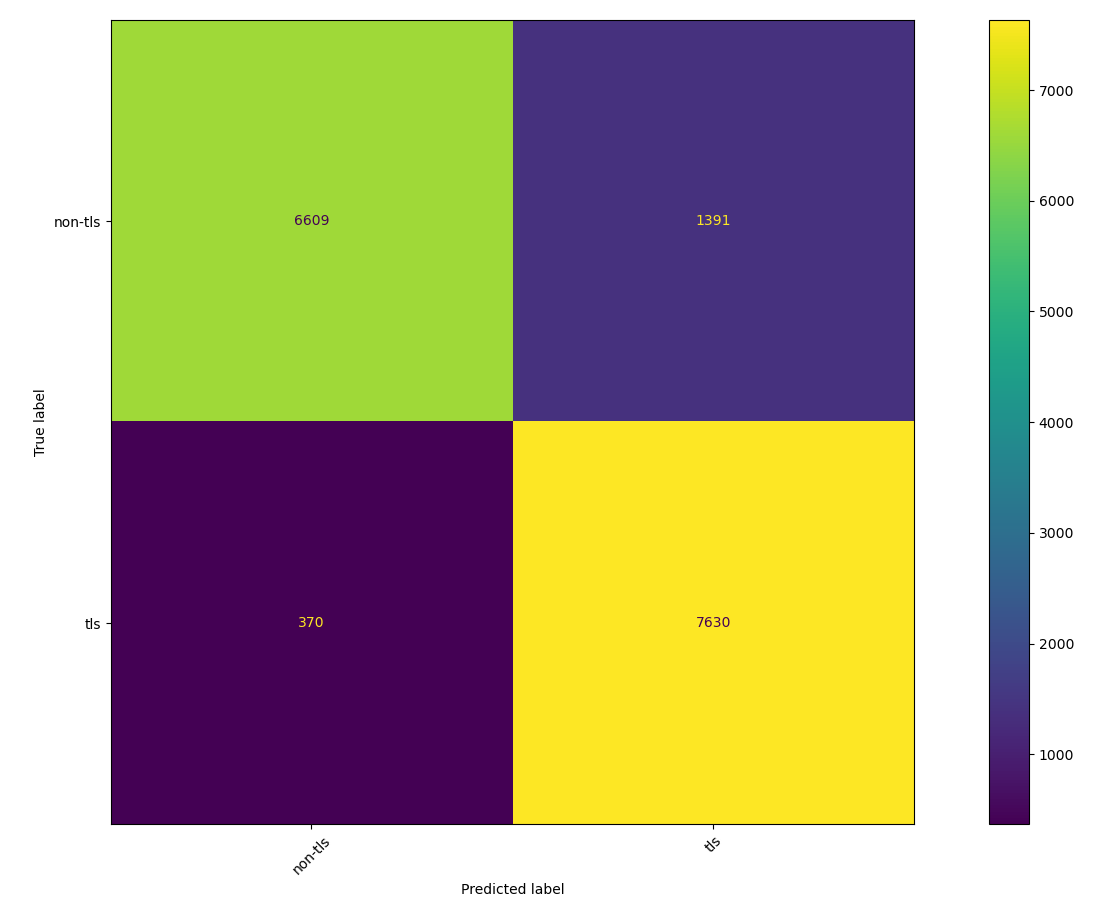
\includegraphics[scale=0.4]{chapters/7/img/tls_nontls.png}
\caption{Plaintext versus encrypted traffic results}
\label{fig:tlsnontls}
\end{figure}

\begin{figure} [ht!]
\centering
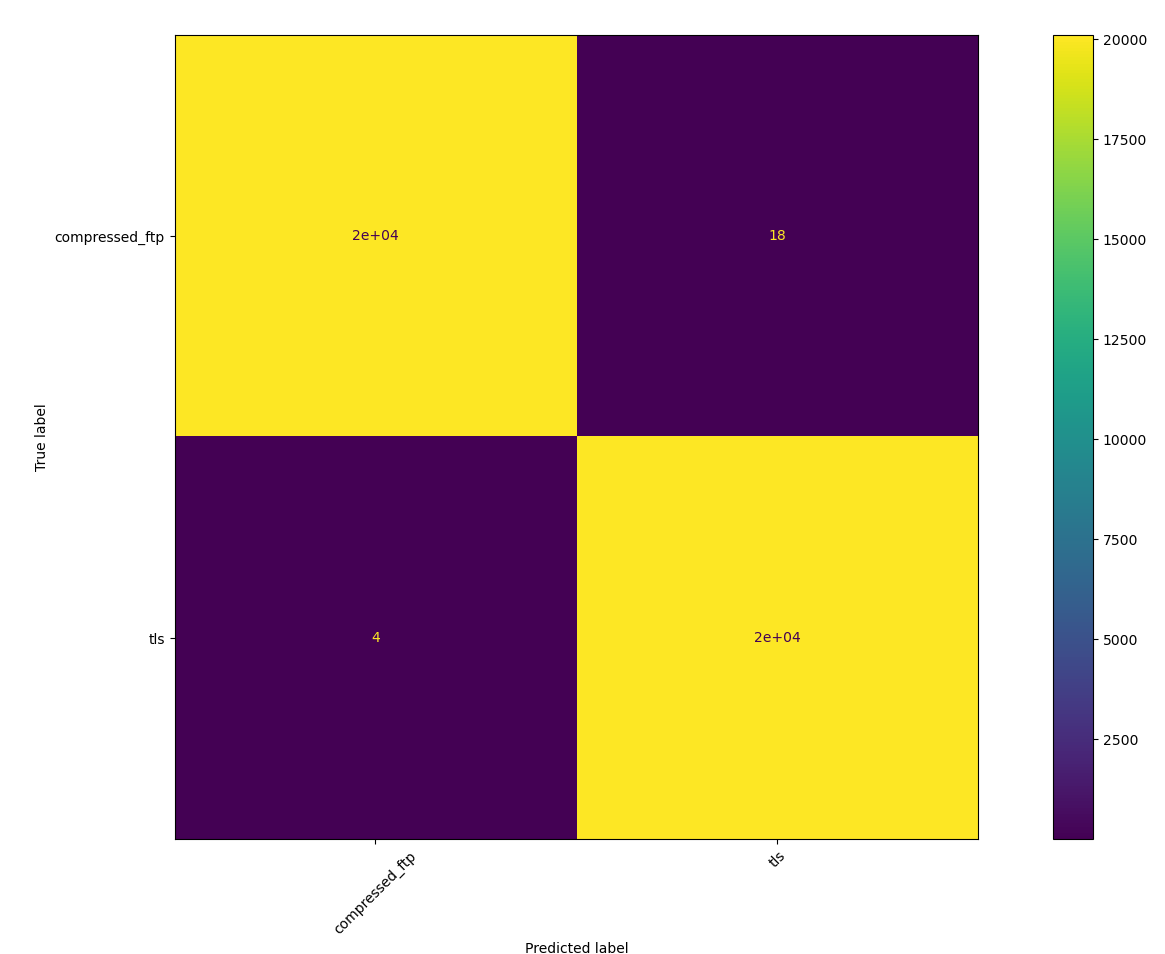
\includegraphics[scale=0.4]{chapters/7/img/compressed_tls.png}
\caption{Compressed versus encrypted traffic results}
\label{fig:tlscomp}
\end{figure}

\begin{figure} [ht!]
\centering
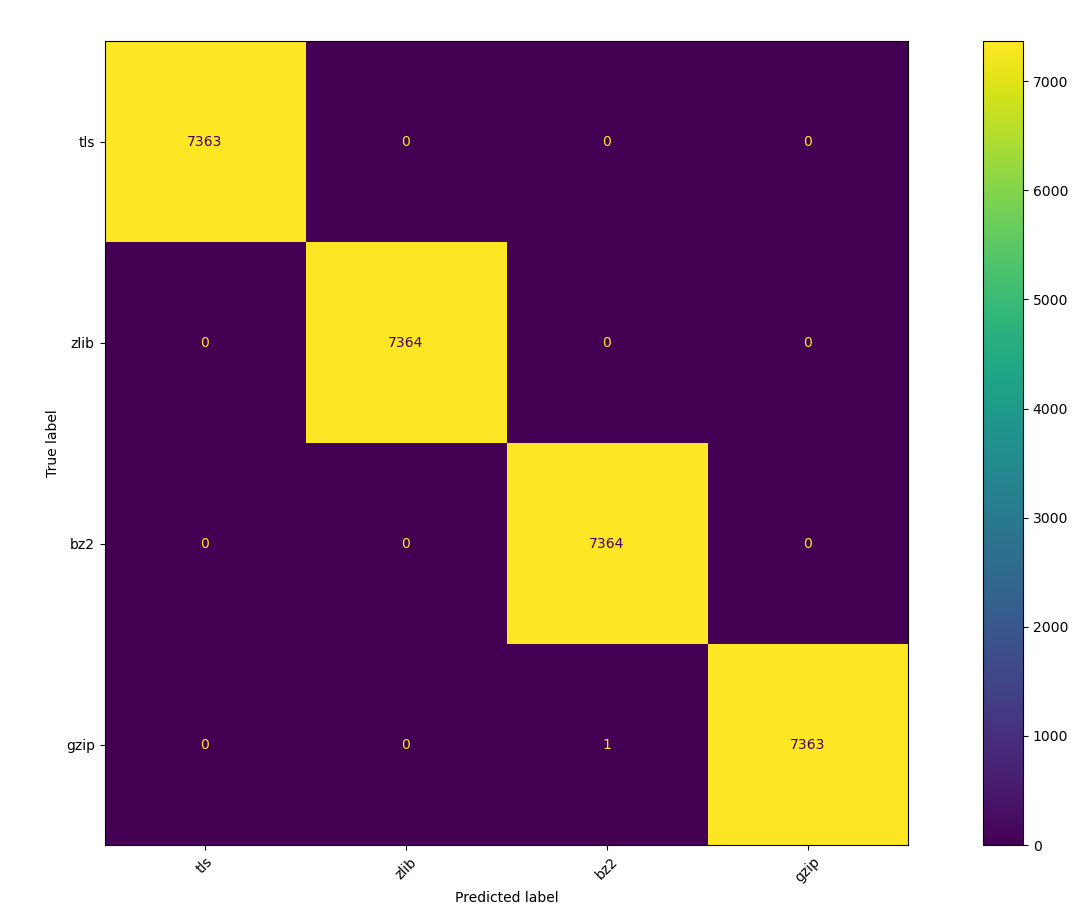
\includegraphics[scale=0.4]{chapters/7/img/encrypted_compressed.png}
\caption{Compression type classification results}
\label{fig:comptype}
\end{figure}


\begin{table}
\centering
\begin{tabular}{| c | p{0.6cm}  p{0.6cm}  p{0.6cm} |}
 \hline
 \textbf{Protocol} & \textbf{P} & \textbf{R} & \textbf{F1}\\
 \hline
 Encrypted & 1.00 & 1.00 & 1.00\\
 Compressed & 1.00 & 1.00 & 1.00\\
 \hline
 Encrypted & 0.85 & 0.95 & 0.90\\
 Plaintext & 0.95 & 0.83 & 0.88\\
 \hline
 TLS & 1.00 & 1.00 & 1.00\\
 BZ2 & 1.00 & 1.00 & 1.00\\
 GZIP & 1.00 & 1.00 & 1.00\\
 ZLIB & 1.00 & 1.00 & 1.00\\
 \hline
\end{tabular}
\caption{Results for encryption and compression detection}
\end{table}

\subsection{SSH over HTTPS}
We want to be able to identify particular instances of certain protocols over an encrypted traffic network; One such protocol of interest is SSH. This is often used to bypass firewall restrictions or create covert data channels. In our experiments, we implemented the same model combinations as with the previous scenarios. The \textsc{Forager} toolkit was highly successful in classifying SSH traffic from the SSH-over-HTTPS dataset generated by the EMews simulator, achieving over 99\% accuracy as shown in Table~\ref{tab:dohsohresults}. Identifying this traffic would allow inspectors to both mitigate covert data channels or monitor them for possible illicit activity. For example, Alice could detect any open covert data channels Bob might attempt to create over SSH.

\subsection{DNS over HTTPS}
Our final experiment was to detect DNS traffic running over HTTPS. A perpetual challenge for security research in classification and anomaly detection is the notion of intent; just because something is identified as belonging to a particular class or marked as an outlier does not always correlate that it is malicious. For example, a new instance of a running process can just be that - a user running a new program - and not necessarily an executing malware. Or a malformed data packet may appear different than others in the stream, but that could just be a bad transmission. For DNS over HTTPS, mainstream browsers like Chrome and Firefox employ this technique without malicious intent. As such, being able to determine DNS tunneling as a second layer to the DoH/non-DoH identification is of critical importance.
 The results in Table~\ref{tab:dohsohresults} show that \textsc{Forager} rises to meet this challenge, and can distinguish both DoH/non-DoH traffic and then malicious traffic from the identified DoH traffic with high accuracy and few false positives. Thus, any attempt Bob makes at DoH tunneling is now detectable using our toolkit.

\begin{table} [ht!]
\centering
\begin{tabular} {|p{2.5cm}|p{2.5cm}|p{2.5cm}|p{2.5cm}|}
\hline
\textbf{Model} & A+P & A+M & A+D \\
\hline
\end{tabular}
\begin{tabular} {|p{2cm}|p{0.6cm}p{0.6cm}p{0.6cm}|p{0.6cm}p{0.6cm}p{0.6cm}|p{0.6cm}p{0.6cm}p{0.6cm}|}
\hline
\textbf{Class} & \textit{P} & \textit{R} & \textit{F1} & \textit{P} & \textit{R} & \textit{F1} & \textit{P} & \textit{R} & \textit{F1} \\
\hline
\hline
\textit{SSH} & 1.00 & 0.99 & 1.00 & 0.98 & 1.00 & 0.99 & 1.00 & 1.00 & 1.00 \\
\textit{Non-SSH} & 0.99 & 1.00 & 1.00 & 1.00 & 0.98 & 0.99 & 1.00 & 1.00 & 1.00 \\
\hline
\hline
\textit{DNS} & 1.00 & 0.97 & 0.98 & 0.96 & 0.99 & 0.98 & 0.95 & 0.99 & 0.97 \\
\textit{Non-DNS} & 0.97 & 1.00 & 0.98 & 0.99 & 0.96 & 0.97 & 0.95 & 0.97 & 0.96 \\
\hline
\hline
\textit{Malicous} & 1.00 & 0.95 & 0.97 & 1.00 & 0.95 & 0.97 & 0.99 & 0.95 & 0.97 \\
\textit{Benign} & 0.96 & 1.00 & 0.98 & 0.95 & 1.00 & 0.97 & 0.96 & 0.99 & 0.97 \\
\hline
\end{tabular}
\caption{Results for classifying DoH/non-DoH and SoH/non-SoH data}
\label{tab:dohsohresults}
\end{table}

\subsection{Performance Metrics}

The experiments were run on a 1.6 GHz Dual-Core Intel Core i5 processor with 16GB of RAM running MacOS Big Sur version 11.6.1. For each of our experiments, we tracked system performance metrics for the models as they performed the classification task and provide this data in Appendix A. This is important for real systems to assess not only the expected tonnage of network traffic they can process, but also to determine what models may be appropriate for deployment. For example, a model whose strategy focuses on online training may not be suitable in an environment who requires high throughput and low downtime, but has a high training time. Or, in some scenarios it may be acceptable to have slightly lower accuracy but a higher throughput rate.

\section{Discussion and Limitations}

Using \textsc{Forager}, we are able to provide new insight into a previously under-analyzed gateway into secure networks - port 443. These techniques enable profiling of encrypted traffic streams while preserving user privacy of the content. We can also use \textsc{Forager} to identify plaintext or compressed traffic from the encrypted streams which may then be forwarded to decompression and DPI tools. Finally, we show the ability of the system to identify not only particular protocols in the encrypted stream, but also distinguish between benign and malicious instances of their utilization. This would be useful, for example, applied in network intrusion detection (NIDS) and prevention systems. For surveillance missions, we show \textsc{Forager} keeps up with the ever-changing, fast-paced real and complex network environment and allows analysts to stay ahead of mission communications and critical data. In seeing through encryption and tunneling, \textsc{Forager} proves to be a versatile solution for real network problems.

For plaintext analysis and keyword searching, using regular expression scanning can still be an effective technique. Automatic generation techniques like RExACtor may also reduce manual overhead required for signature creation and maintenance, and provide useful insight to commonalities across traffic types and protocols. Additional regular expression scanning and generation tools would be a useful addition to the \textsc{Forager} toolkit.


\chapter{CONTRIBUTIONS AND DELIVERABLES}

We designed the \textsc{Forager} toolkit as a usable software package for reproducability and further community research. This software is a command line interface (CLI) application installed through PyPi with user documentation provided through ReadTheDocs. The source code repositories are also available through GitHub with open-source licensing. The following components are included in the initial 1.0 release:

\medskip

\textbf{TaPCAP: } This option parses input PCAP and PCAPNG files, extracting header features and/or payloads into CSV format. This module can be installed separately~\footnote{https://pypi.org/project/tapcap/} or run from \textsc{Forager}.

\textbf{\textsc{RExACtor}: } The token option finds frequent tokens according to a provided threshold from a CSV output from \textsc{Tapcap}. The regular expression mode performs genetic sequencing alignment of payloads from a CSV output from \textsc{Tapcap}. \textsc{Rexactor} can be installed as a separate component~\footnote{https://pypi.org/project/rexactor/} or run from \textsc{Forager}.

\textbf{\textsc{Alpine}: } In training mode, this model accepts as input the CSV obtained from \textsc{Tapcap}, generates locality sensitive hashes from the header data, and finalizes and serializes these to an LSHForest~\cite{lshforest}. In testing mode, the trained LSHForest is reloaded from the internal cache. Locality sensitive hashes of the input data are generated and index lookup performed. The returned result is applied to the ensemble voting system if other models are configured.

\textbf{\textsc{Palm}: } In training mode, this model accepts as input the CSV obtained from \textsc{Tapcap}, generates locality sensitive hashes from the payload data, and finalizes and serializes these to an LSHForest~\cite{lshforest}. In testing mode, the trained LSHForest is reloaded from the internal cache. Locality sensitive hashes of the input data is generated and index lookup performed. The returned result is applied to the ensemble voting system if other models are configured.

\textbf{\textsc{Maple}: } In training mode, this model accepts as input the CSV obtained from \textsc{Tapcap}, generates grayscale images from the payload data, and saves the generated neural network model and trained weights to JSON and H5 files, respectively. In testing mode, the trained neural network is reloaded from the internal cache. Grayscale images of the input data are generated and used as input to the CNN classifier. The returned result is then applied to the ensemble voting system if other models are configured.

\textbf{\textsc{Date}: } In training mode, this model accepts as input the CSV obtained from \textsc{Tapcap}, generates point clouds from the payload data and performs DBSCAN analysis. It then saves the generated neural network model and trained weights to JSON and H5 files, respectively. In testing mode, the trained neural network and weights are reloaded from the internal cache. Point clouds are generated from input data and DBSCAN analysis performed, and this is used as input to the multi-layer perceptron classifier. The returned result is applied to the ensemble voting system if other models are configured.

\textbf{Multi-modality: } \textsc{Forager} supports training and using one or more of the \textsc{Alpine}, \textsc{Palm}, \textsc{Maple}, and \textsc{Date} models together so that the packet may be analyzed from multiple representations. We use votes in a combined ensemble classifier and return the class with the most votes as the final classification.


\chapter{CONCLUSIONS}

\section{Future Work}
The scope of this dissertation includes the research and methods leading to the initial release of the Forager toolkit. This work focuses on per packet inspection and data transformation techniques which are viable for large-scale deployments. There are a number of flow-based techniques referenced in this work which do have practical applications. Netflow data is often used in recurrent neural network or long short-term memory network analysis and can be extracted often with ease from routers, switches, or other network devices. A future expansion of this toolkit would be the ability to process netflow or other such stream-based data or cross-packet features when available.

There are also many deep learning and data mining techniques which we have not yet covered but have been explored in other works. Principle component analysis (PCA)~\cite{Yan2014Principal, Nilesh2021machine} and eigenvectors~\cite{Qing2021Encrypted} have been used in per packet classification with success. These techniques are notably efficient and therefore would be excellent candidates for additional features in a future release for processing at large scale.

While we found that adjusting for TF-IDF score in \textsc{Palm} did not improve classification accuracy in the experiments we ran, there are applications for other natural language processing and word embedding techniques in the literature on traffic classification. Word embeddings can be used to classify real versus fake domain names~\cite{Vinayakumar2020visualized}, phishing emails~\cite{rao2022application,  yuan2018url2vec, tajaddodianfar2020texception} and other kinds of phishing attacks~\cite{somesha2022classification}, and HTTP traffic~\cite{gniewkowski2021http2vec}. In the cybersecurity domain, Word2Vec has been used to identify cross-site scripting~\cite{fang2018deepxss, guichang2019cnnpayl} and SQL injection attacks~\cite{yu2019detecting} across network packets. Textual analysis is rendered ineffective by encryption and compression in many cases, but for plaintext analysis or malware detection could be a future approach.

The data itself we chose to work with in these experiments until \textsc{Forager}'s initial release has largely been sourced from traditional network devices. Mobile traffic and data gathered from IoT or medical/wearable devices could present unique challenges and opportunities for classification problems. In future versions of this toolkit, we could leverage the dimensionality reduction offered by our data engineering and mining techniques in order to combine feature sets and further increase multimodality. For example, we could embed both the processing power and CPU utilization of an IoT device input along with network traffic embeddings to further inform a classification of IoT devices. There is also much opportunity for experimentation with classifying streams of traffic in multiple ways. As mentioned in the introduction of this work, traffic classification covers a broad scope of problems; importantly, these classes are not distinct from one another and traffic may belong to multiple classes and it may be necessary to classify something multiple times. For example, we may want to determine the user who generated a traffic stream (Bob), what protocols are in the traffic (SIP, RTP), what application Bob used to generate the traffic (Zoom), and what device of Bob's he used to make the call (MacBook Air). Determining methods to perform multiple classifications like this without re-processing the data each time would be a useful additional contribution.

\section{Summarization}
This work proposes a new system of data mining and deep learning for network traffic classification at scale. The \textsc{Forager} system includes models which contribute both novel application of data transformation techniques which unveil hidden representations as well as machine learning models applied in real systems. We propose a method for extracting data from PCAPs and converting them to tabular format, then transforming them appropriately according to what we have learned from previous experiments. For example, plaintext, strongly signatured data which we are aiming to identify by protocol (SIP, HTTP, POP) may be aptly suited for regular expression generation algorithms. Alternatively, weakly signatured data may be run with the \textsc{Maple} model for payload analysis and \textsc{Alpine} model for header features for identification. Similarly for profiling, encrypted data may also be well-suited for the \textsc{Alpine} and \textsc{Maple} model combination. Our ensemble voting system allows for this multimodal analysis and can finally be saved and returned through a tagging system implemented in the original data. Thus, our toolkit will be a useful contribution to network analysts and cybersecurity and surveillance specialists for uniquely identifying traffic on the internet today.


\fbmatterchapterformat

\bibliographystyle{ieeetr}
\bibliography{references}


\newpage{}\uncctocformat{chapter}{0pt}{350pt}{\appendixname~\thecontentslabel:~}
\renewcommand{\chaptertitlename}{APPENDIX}
%
% The default setting for appendices excludes sections, subsections, etc. from
% the TABLE OF CONTENTS.
% If you want these in the TABLE OF CONTENTS, increase the number in the line below:
% 1 - Appendices, Sections / 2 - Appendices, Sections, Subsections / 3 - etc
%
\addtocontents{toc}{\protect\setcounter{tocdepth}{0}}

\appendix

\end{document}
